\documentclass[letterpaper, 12pt]{article}

\usepackage{caption}
\usepackage{float}
\usepackage[T1]{fontenc}
\usepackage[lmargin=1 in, rmargin=1 in, tmargin=1 in, bmargin=1 in]{geometry}
\usepackage{graphicx}
\usepackage{hyperref}
\usepackage{times}
\usepackage{xcolor}

\begin{document}

\textbf{Reviewer 1}

\bigskip

\textit{My main comment concerns the bias in the observation of S minus P times. The authors measure the observed lag time from the centroid of the cross-correlation function within the time window 2 seconds before and after the theoretical lag time if the tremor source was on the plate boundary (L330-335). I understand that such kind of constraint is sometimes useful for obtaining realistic solutions, but I am worried whether this constraint works for too strong bias that concentrates all tremor depths to the plate boundary depths. In other words, the S minus P time measurements should be free from theoretical time lags when discussing the spatial relationship between tremor and plate boundary. How about using the whole time window or focusing on the window around the maximum peak? In any case, the authors should check and show that these time window limitations do not strongly affect the results.}

\bigskip

You bring up a very important point regarding the potential of bias in our results and we have explored this in some detail.  We have rewritten our method to include an important detail that we left out of the text of the submitted version which we now explain on lines 263-275.  We have also sent figures to show more clearly the windows we analyze for the clustering relative to the theoretical time and our final observation.  The highest peak in the absolute value of the phase-weighted stacks of the cross correlation functions $S_i(\tau)$ within the defined window is the same as the highest peak between 3 and  8 seconds for every array / tremor grid  except for one (BH 5, -5) so using the theoretical S-P time as a guide to define the time window has very little or no effect on the final travel-time observation. 

\smallskip

The width of the time window selected to compute the moment centroid may have an effect on the estimation of the depth of the tremor. To verify this, we varied the width of the time window and computed the corresponding variations of the depth of the tremor. We added this discussion in the text at lines 368-377.

\bigskip

\textit{Thickness or depth extent of tremor sources in this study is derived from the scattering of time lags or depths for one-minute-long time windows (L414-438). However, none of the time lag or depth distribution for one-minute-long time windows are presented in the manuscript. I recommend showing at least some examples of these distributions. Besides, I am not (and probably most readers would not be) familiar with Qn estimator. Please give a more detailed explanation about what Qn estimator is and in which case it works well (compared with MAD).}

\bigskip

We added an example of distribution of time lags in the supplement. We added a description of the Qn estimator and its advantage compared to the MAD in the text.

\bigskip

\textit{L194: Ghosh et al., 2010 -> Ghosh et al., 2010ab?}

\textit{L306: Ghosh et al., 2010 -> Ghosh et al., 2010b?}

\bigskip

We modified the reference.

\bigskip

\textit{L330: I cannot get the meaning of the sentence, "We considered only the horizontal component with the maximum value of the peak". Do you select the EW or NS components with the larger maximum value of the peak?}

\bigskip

Yes, we select the component (EW or NS) that has the largest maximum value of the peak. We modified this sentence in the text.

\bigskip

\textit{L346-358: half width is a typical measure for uncertainties when picking a peak value. In this case, when picking a centroid value, it is more natural to use standard deviation or MAD (or Qn?).}

\bigskip

Here we wanted to make the distinction between a sharp peak and a flatter peak which could have the same moment centroid. This is why we choose the half-width.

\bigskip

\textit{L375: different different -> different}

\bigskip

We corrected this sentence.

\bigskip

\textit{L468-474: I think this paragraph is not an important conclusion of this work and is already placed in the Discussion just above the Conclusion. No need to repeat here.}

\bigskip

We deleted this paragraph.

\bigskip

\textit{Figure 6, Figure 8, Figure 11, Figure 12: Please consider changing the symbol of Three Bumps (triangles). They are the same symbol as the array positions in Figure 1 and are a bit confusing.}

\bigskip

We modified the symbols for Three Bumps.

\bigskip

\textbf{Reviewer 2}

\bigskip

\textit{I have only one minor quibble: in lines 443 - 445 the authors state "The depth range of the tremor is larger than the depth range of the low-frequency earthquakes, but this may be due to the uncertainty of the determination of the tremor depth." As far as I can tell, the depth range of members of an LFE family was not measured by Chestler and Creager (2017). Their three models assume a planar structure. A recent JGR paper by Sammis and Bostock (2021) proposed that LFEs beneath Vancouver Island occur at the sites of granular jams in a flow channel between 0.5 and 1.5 kilometers thick. So, the assumption of a planar distribution of LFEs in a family may be premature.}

\bigskip

There are two papers by Chestler and Creager in 2017. We added the reference in the text. Here, we are considering the range over all LFE families of the distance between the location of the LFE family and the plate boundary, not the depth range of the source of the LFEs within a single LFE family. The LFE families are close to the plate boundary, but not exactly on a plane. We modified the text and we added the comparison with the thickness of the flow channel.

\bigskip

\textbf{Additional figures related to first comment from Reviewer 1}

\bigskip

\begin{figure}
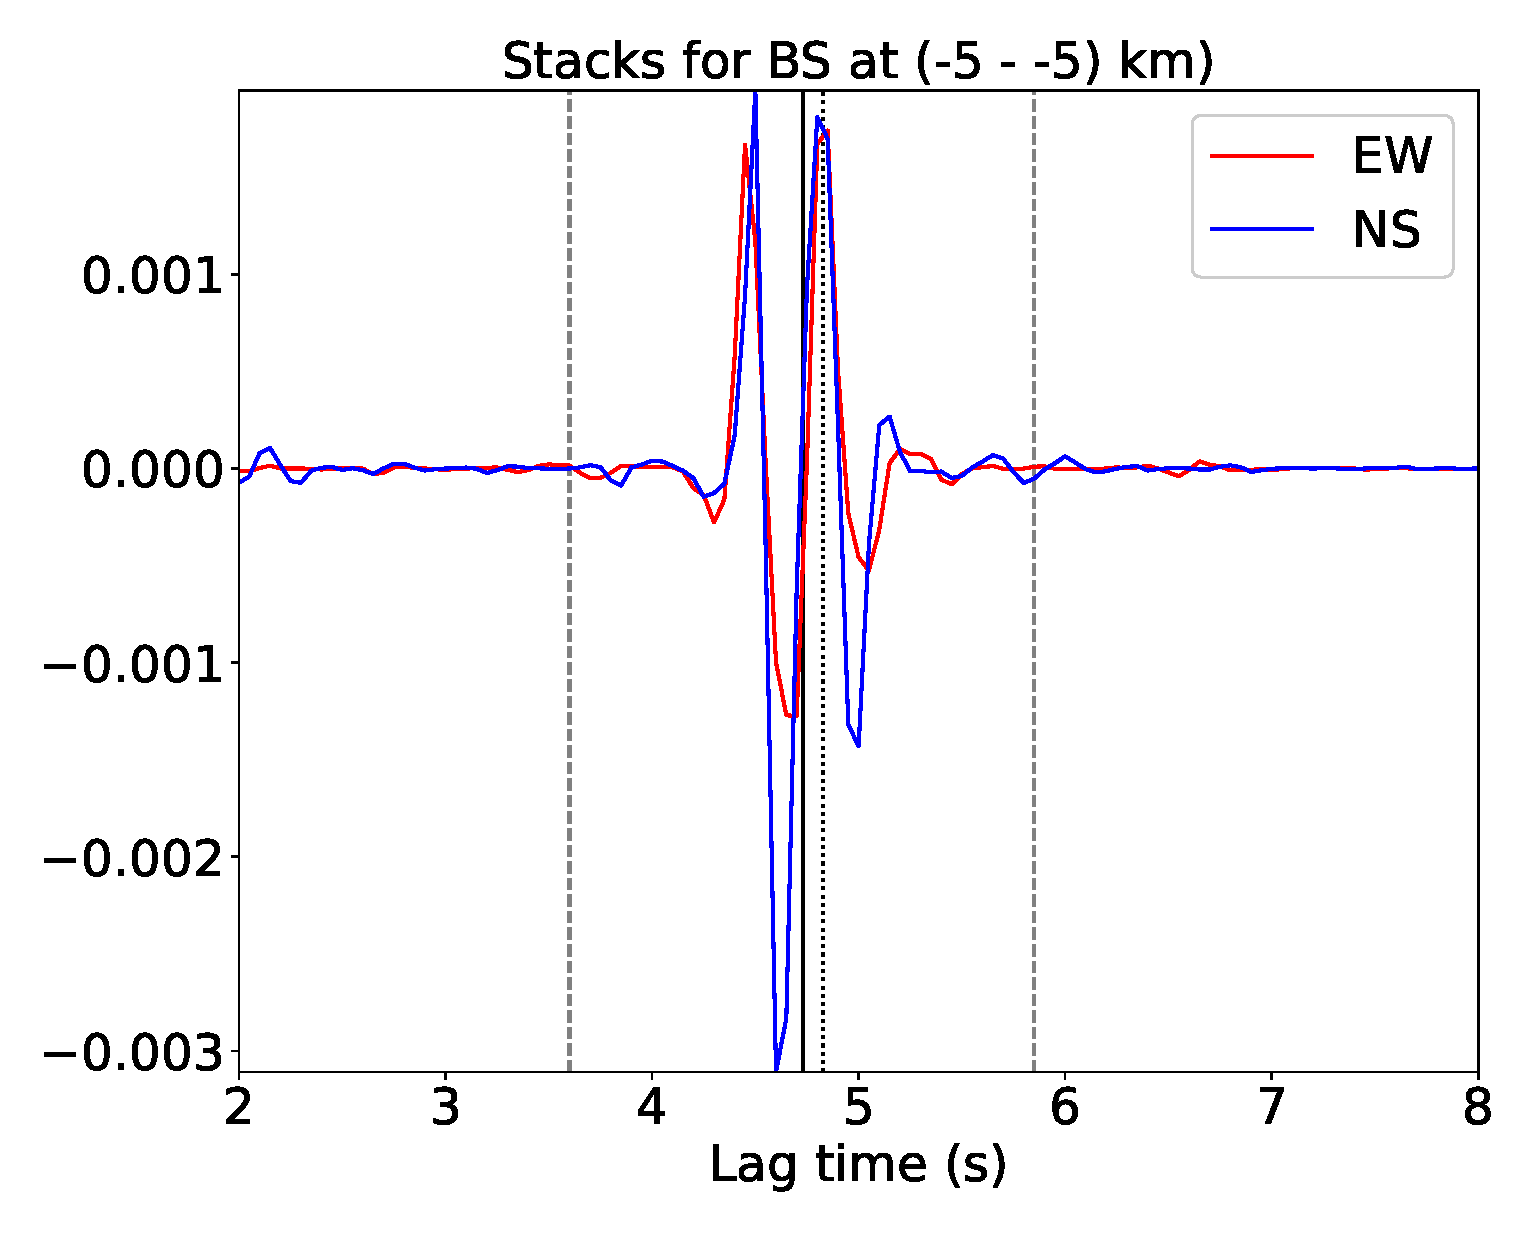
\includegraphics[width=\linewidth]{figures/intervals/BS_-05_-05_stacks.eps}
\caption{Stack of the cross-correlation functions for the Big Skidder array for the 110 one-minute long time windows when tremor was detected in a 5 km by 5 km grid cell located 7 kilometers southwest of the array. Red line corresponds to the cross-correlation of the East-West component with the vertical component, and blue line corresponds to the cross-correlation of the North-South component with the vertical component. The solid black line corresponds to the final observed S-P time, the black dotted line is the theoretical SP time if the source is on the plate boundary, and the grey dashed lines are the intervals $\left[T_{min} ; T_{max}\right]$ where we look for a secondary peak. For all the remaining figures, the two letters abbreviation in the title corresponds to the name of the array, and the numbers in parenthesis indicate the distance from the array to the grid cell in the east direction and the north direction.}
\end{figure}

\begin{figure}[H]
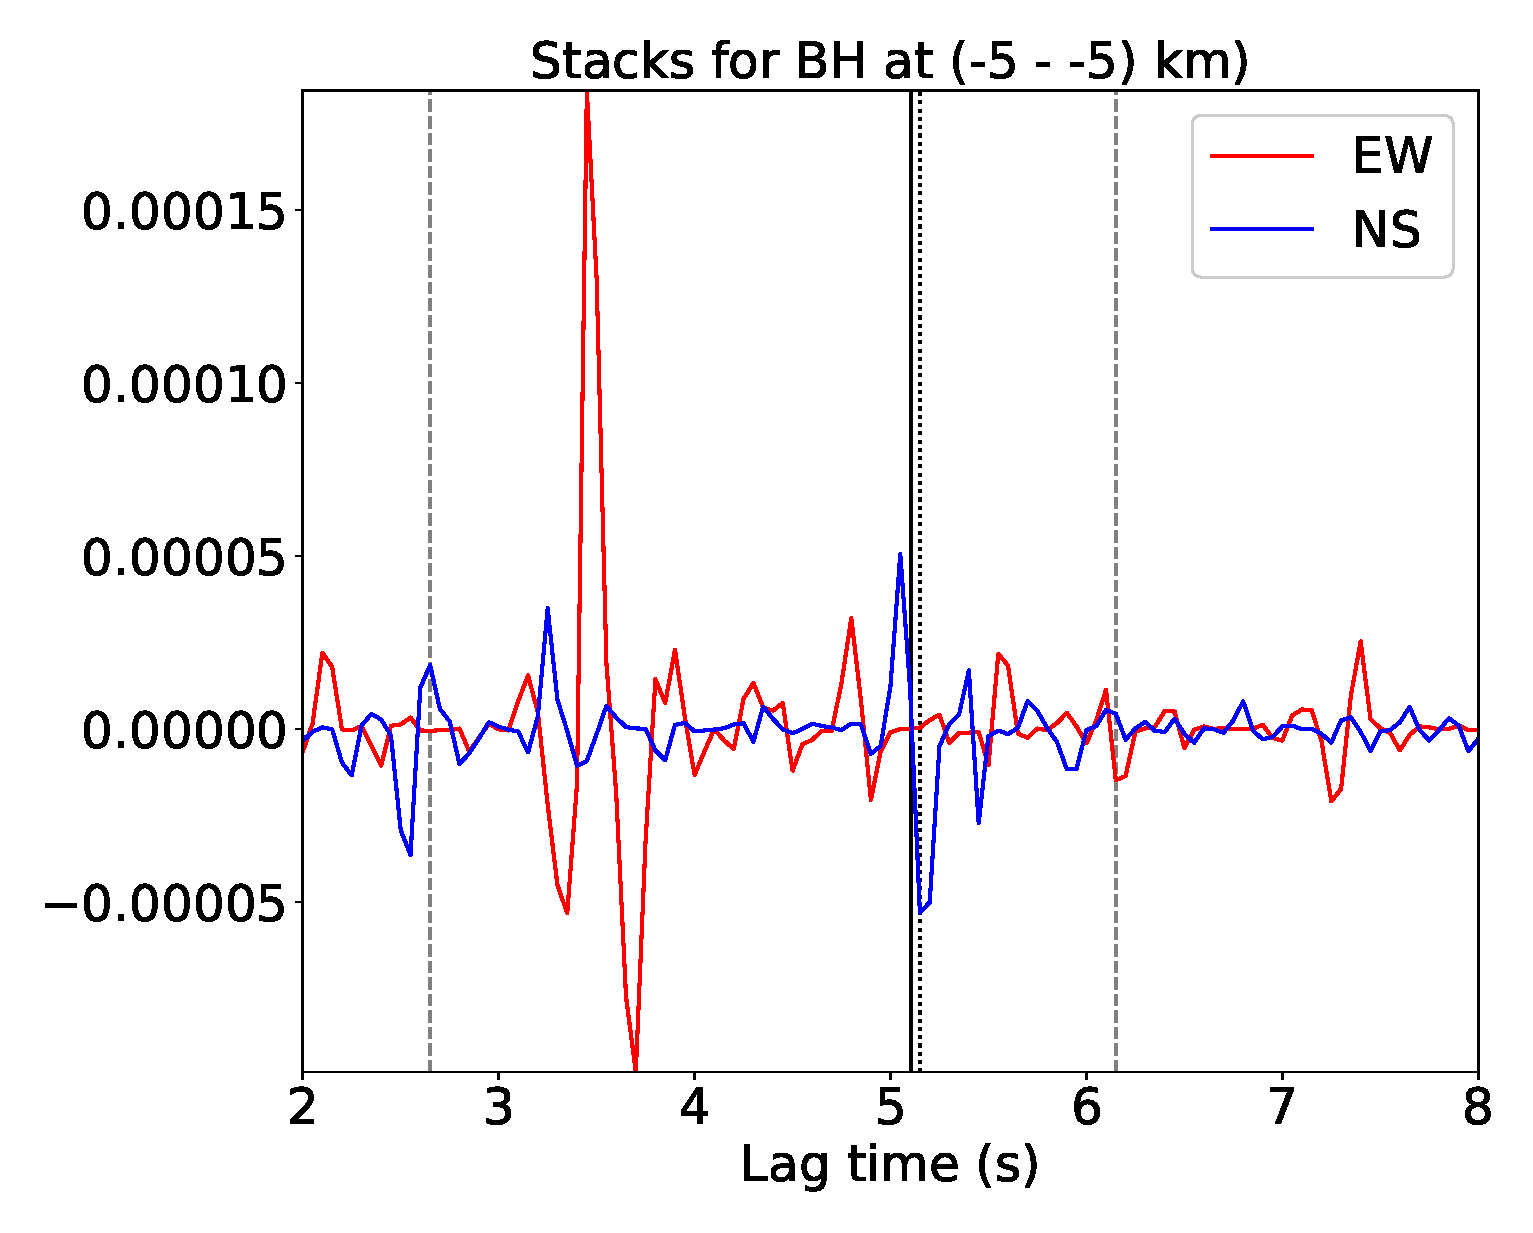
\includegraphics[width=\linewidth]{figures/intervals/BH_-05_-05_stacks.eps}
\caption{See caption of Figure 1 for an explanation of this figure.}
\end{figure}

\begin{figure}[H]
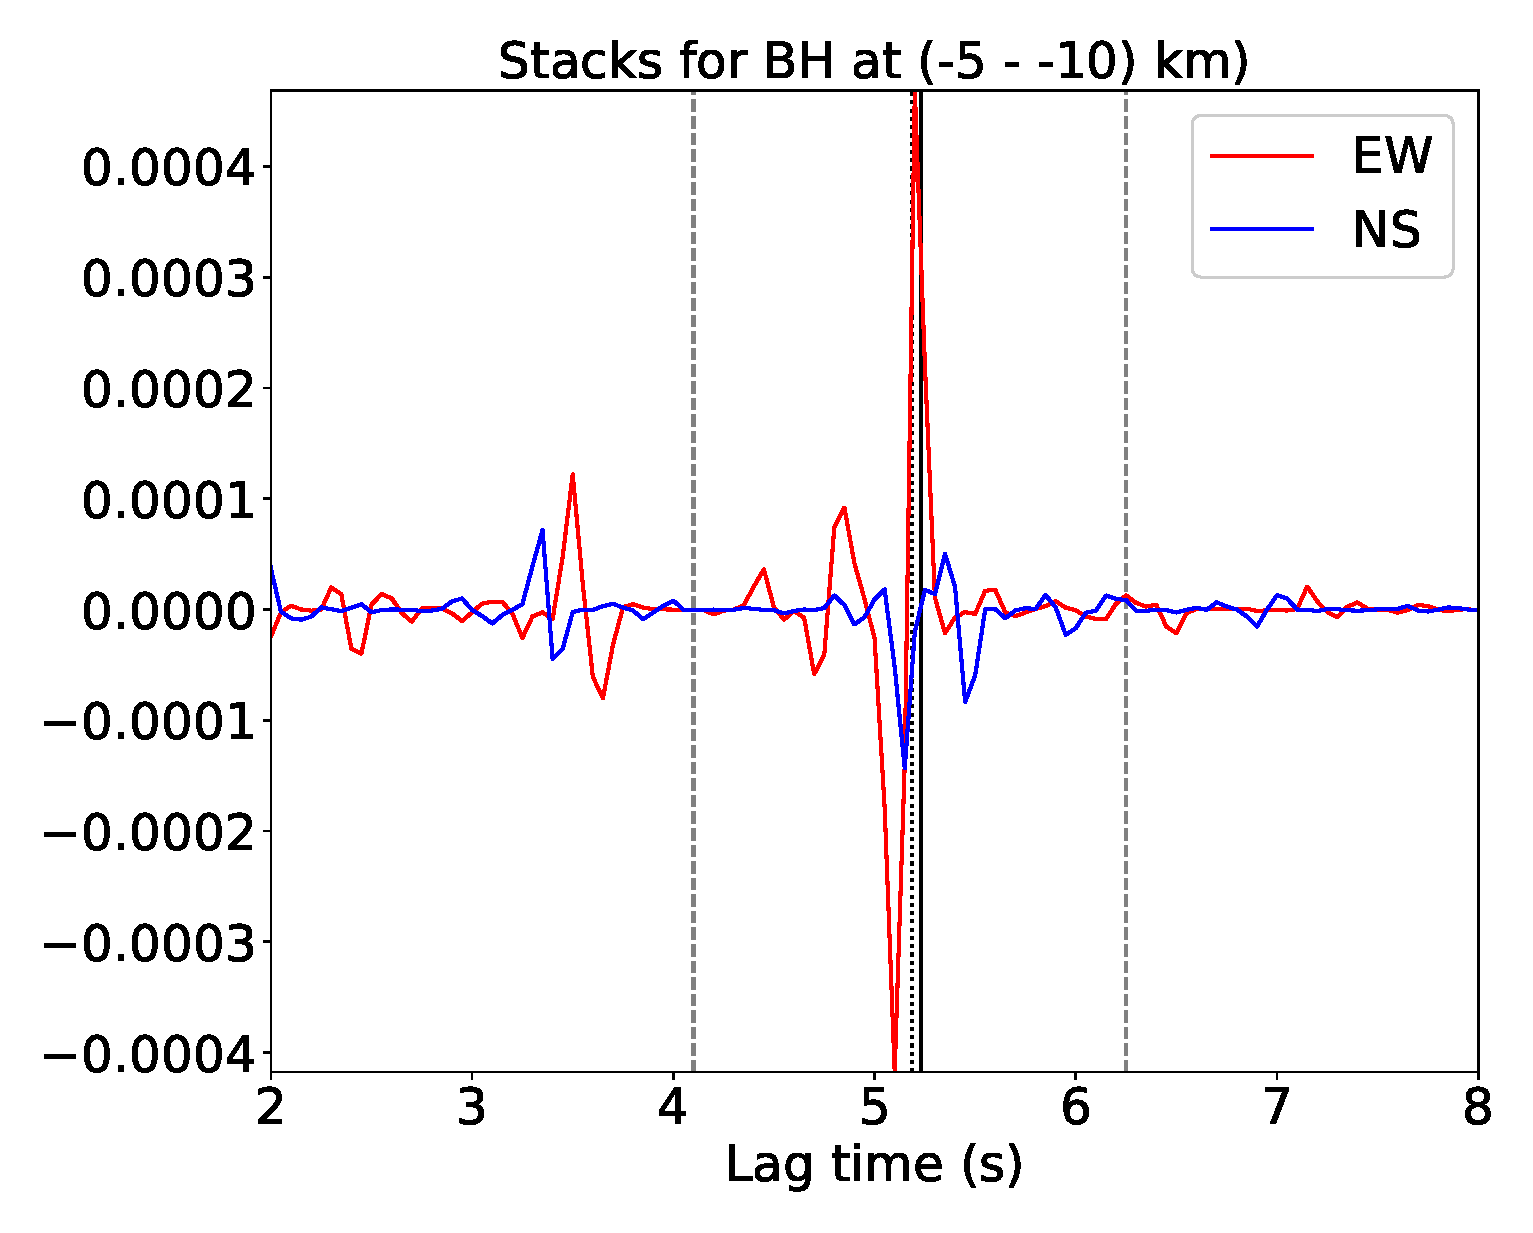
\includegraphics[width=\linewidth]{figures/intervals/BH_-05_-10_stacks.eps}
\caption{See caption of Figure 1 for an explanation of this figure.}
\end{figure}

\begin{figure}[H]
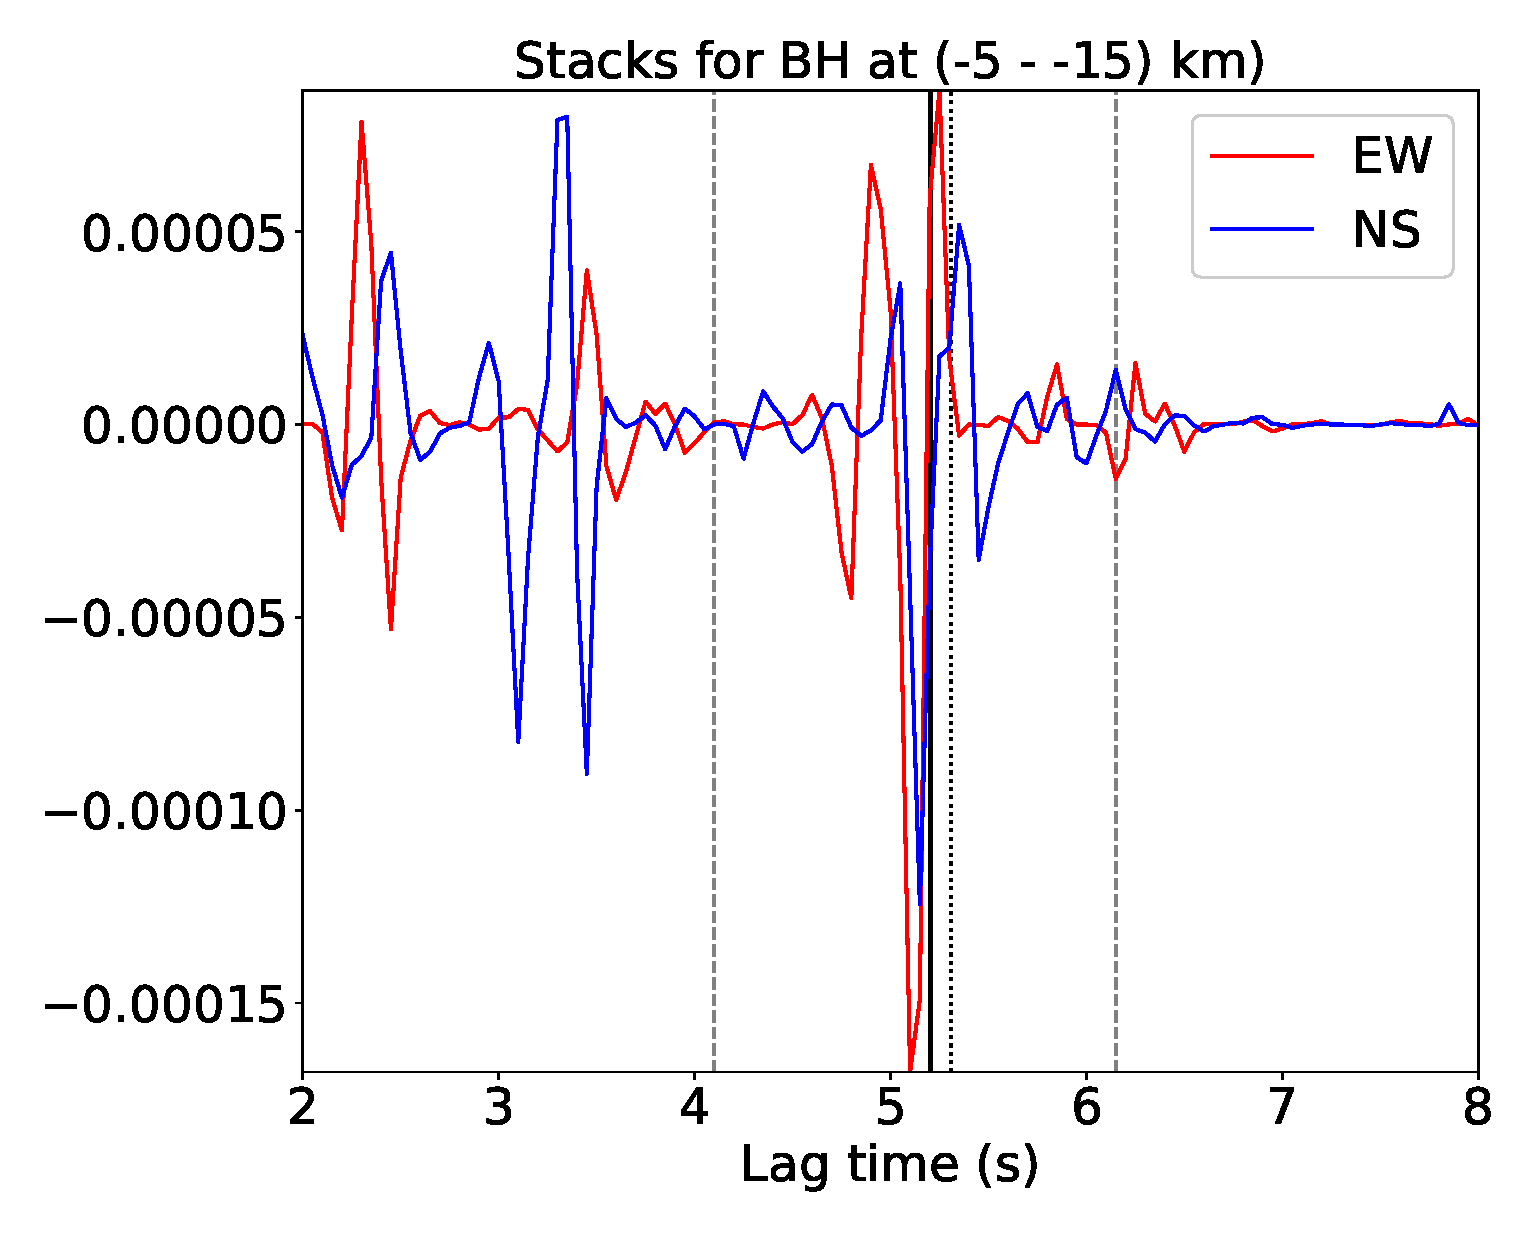
\includegraphics[width=\linewidth]{figures/intervals/BH_-05_-15_stacks.eps}
\caption{See caption of Figure 1 for an explanation of this figure.}
\end{figure}

\begin{figure}[H]
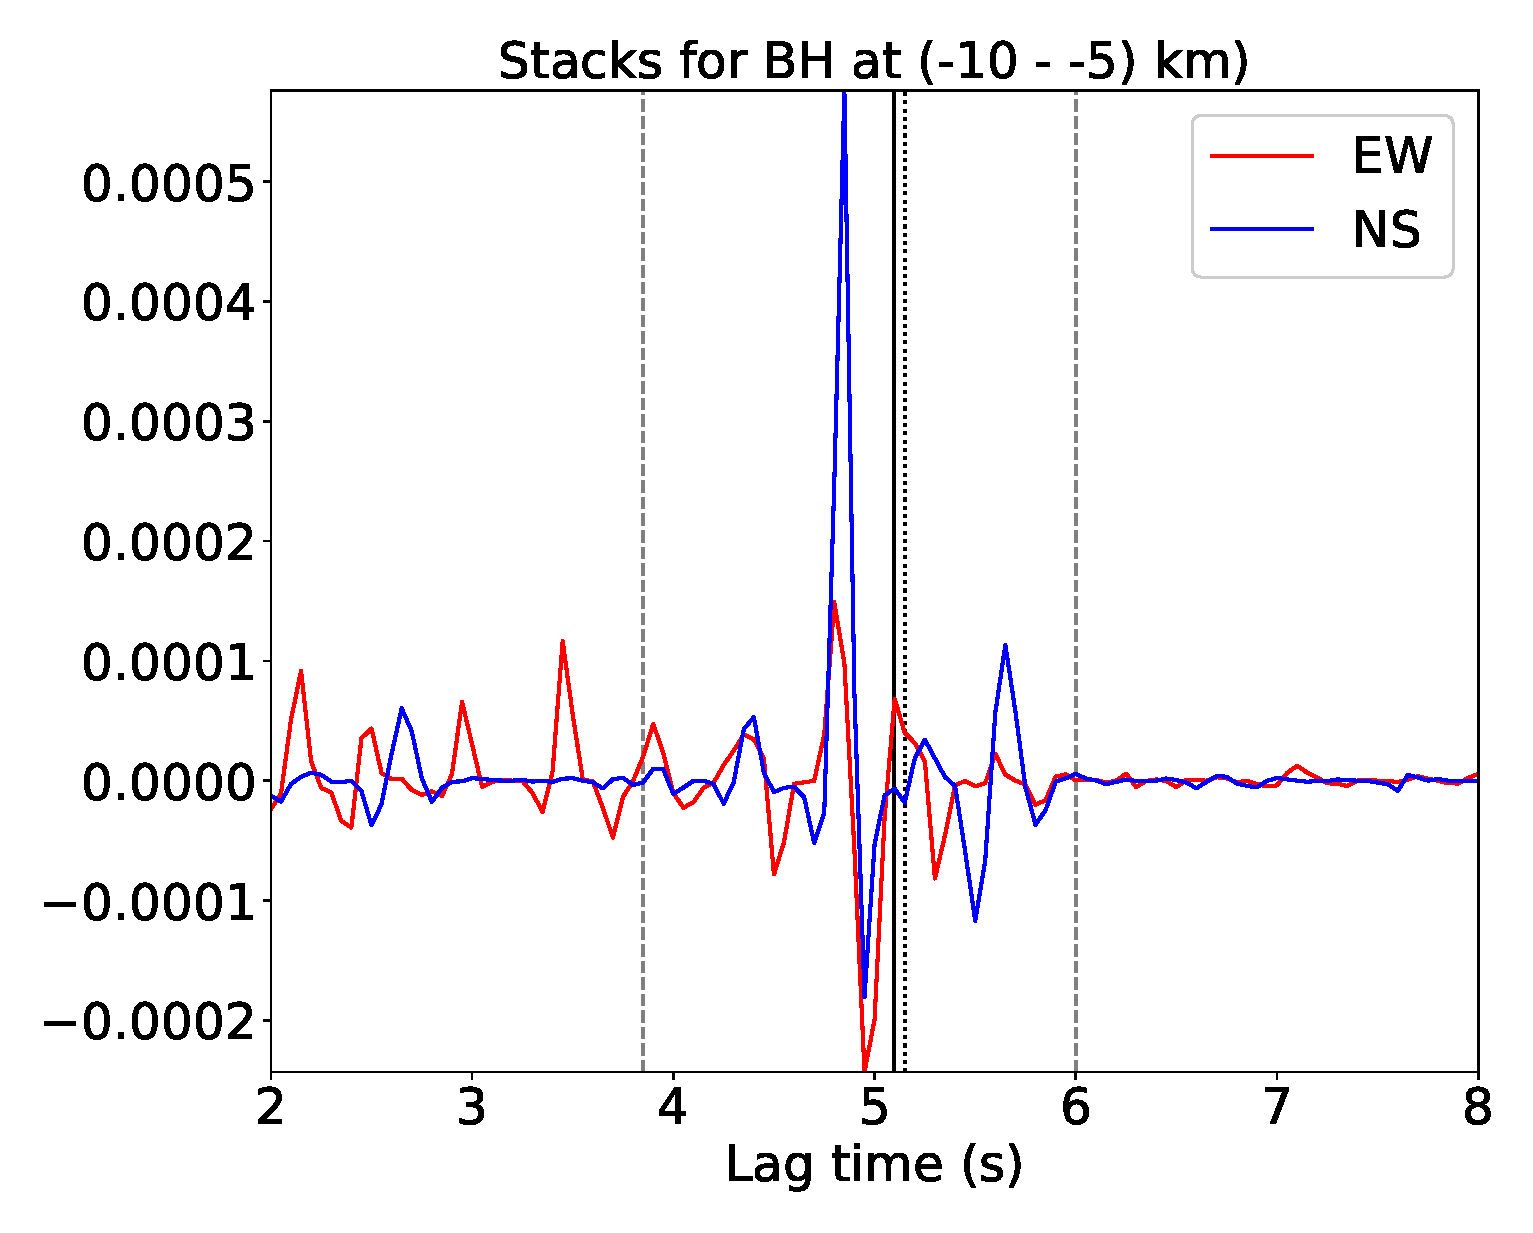
\includegraphics[width=\linewidth]{figures/intervals/BH_-10_-05_stacks.eps}
\caption{See caption of Figure 1 for an explanation of this figure.}
\end{figure}

\begin{figure}[H]
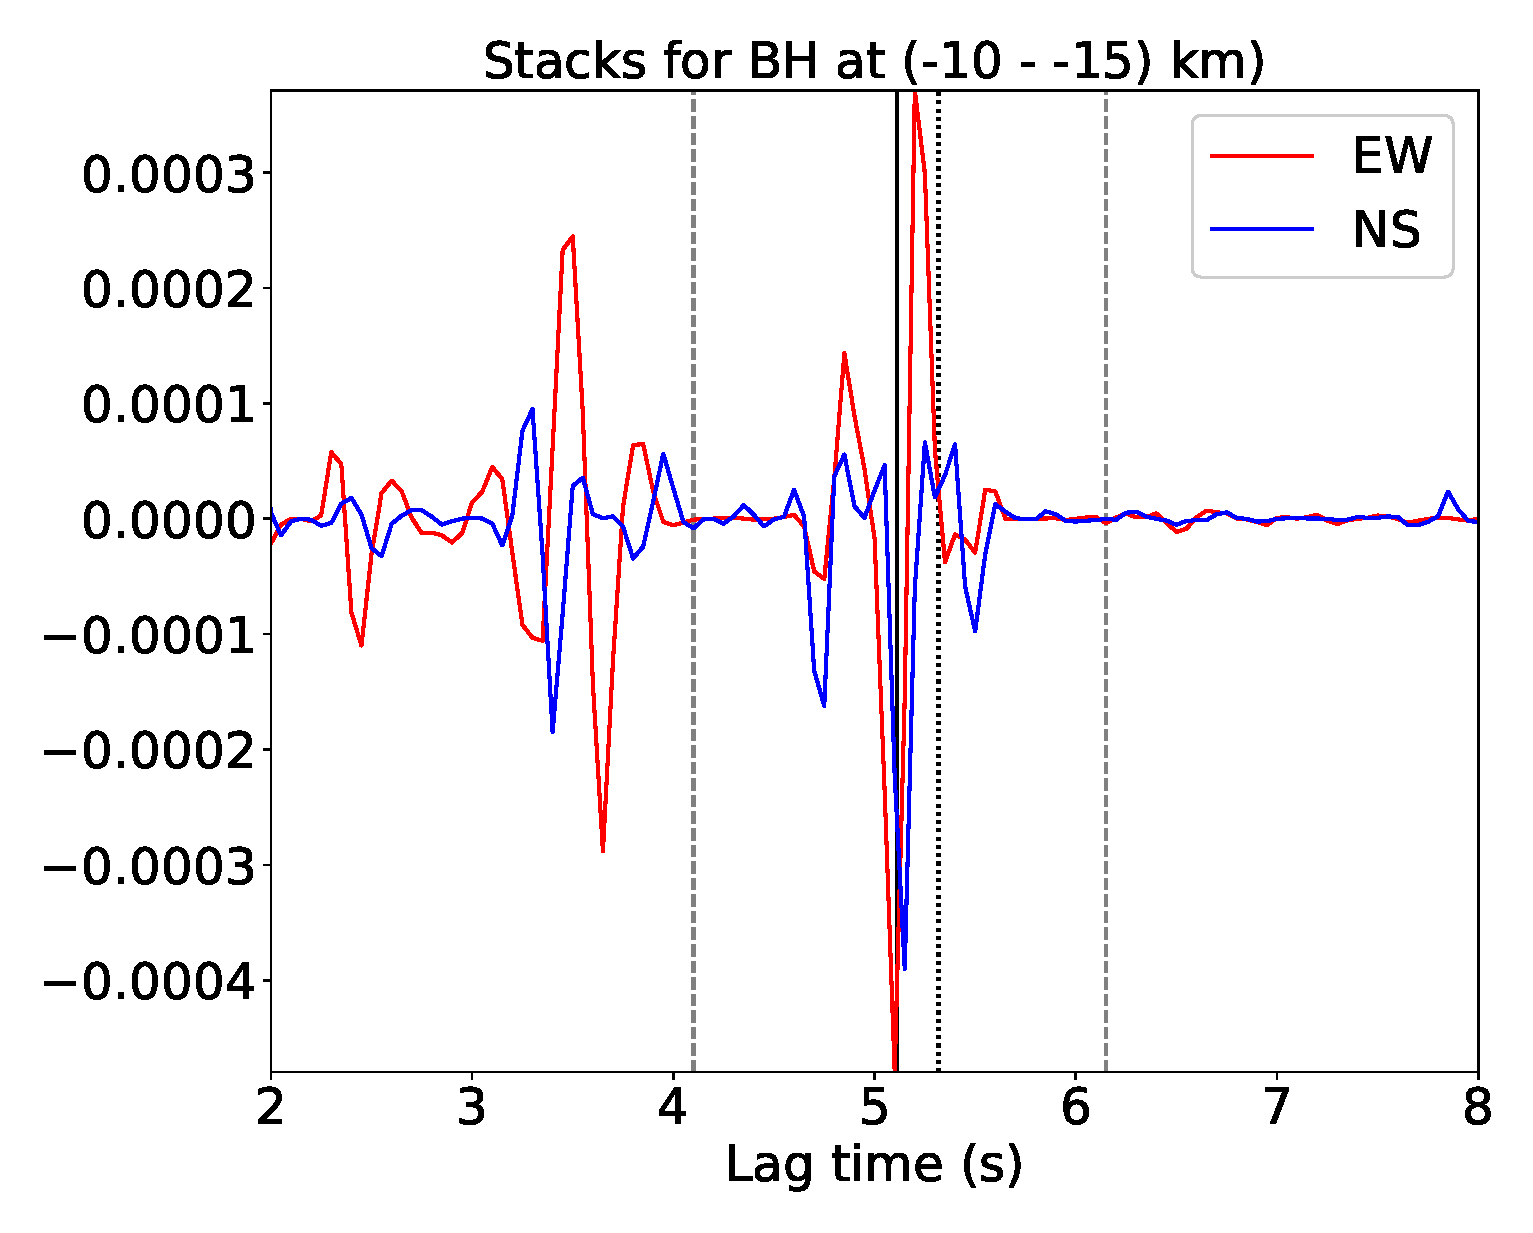
\includegraphics[width=\linewidth]{figures/intervals/BH_-10_-15_stacks.eps}
\caption{See caption of Figure 1 for an explanation of this figure.}
\end{figure}

\begin{figure}[H]
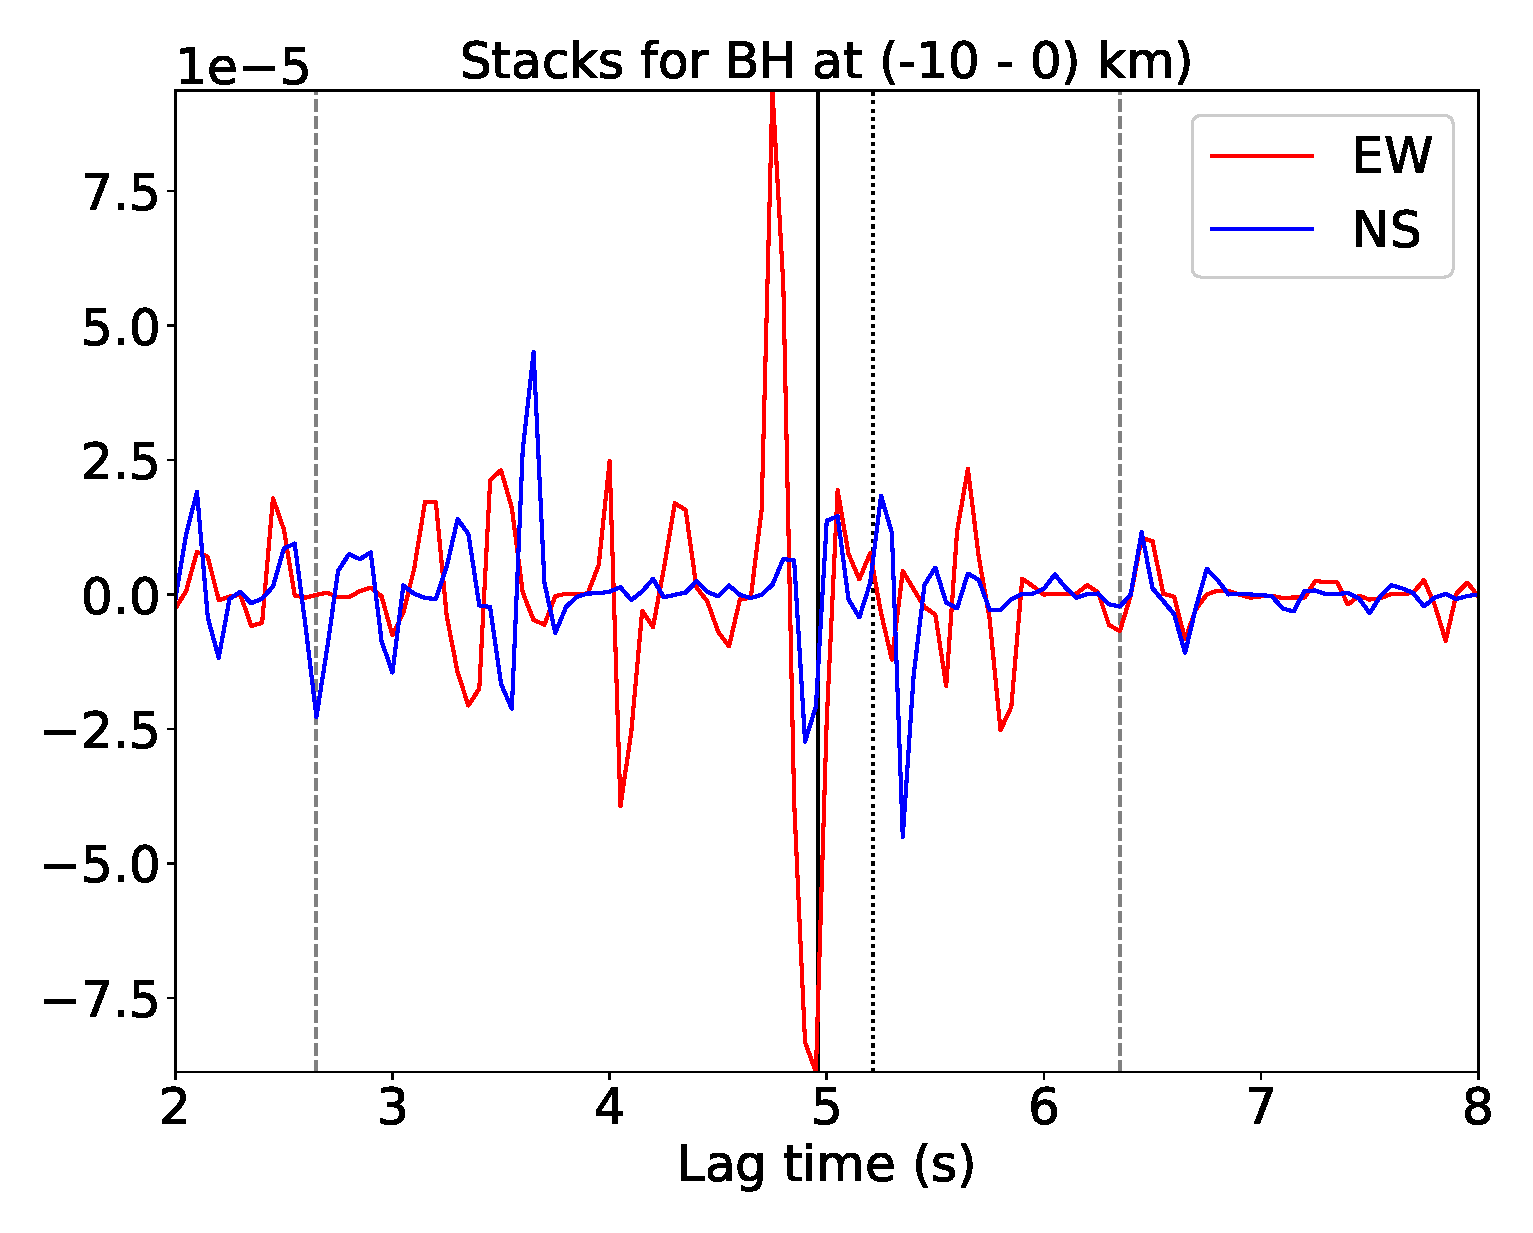
\includegraphics[width=\linewidth]{figures/intervals/BH_-10_000_stacks.eps}
\caption{See caption of Figure 1 for an explanation of this figure.}
\end{figure}

\begin{figure}[H]
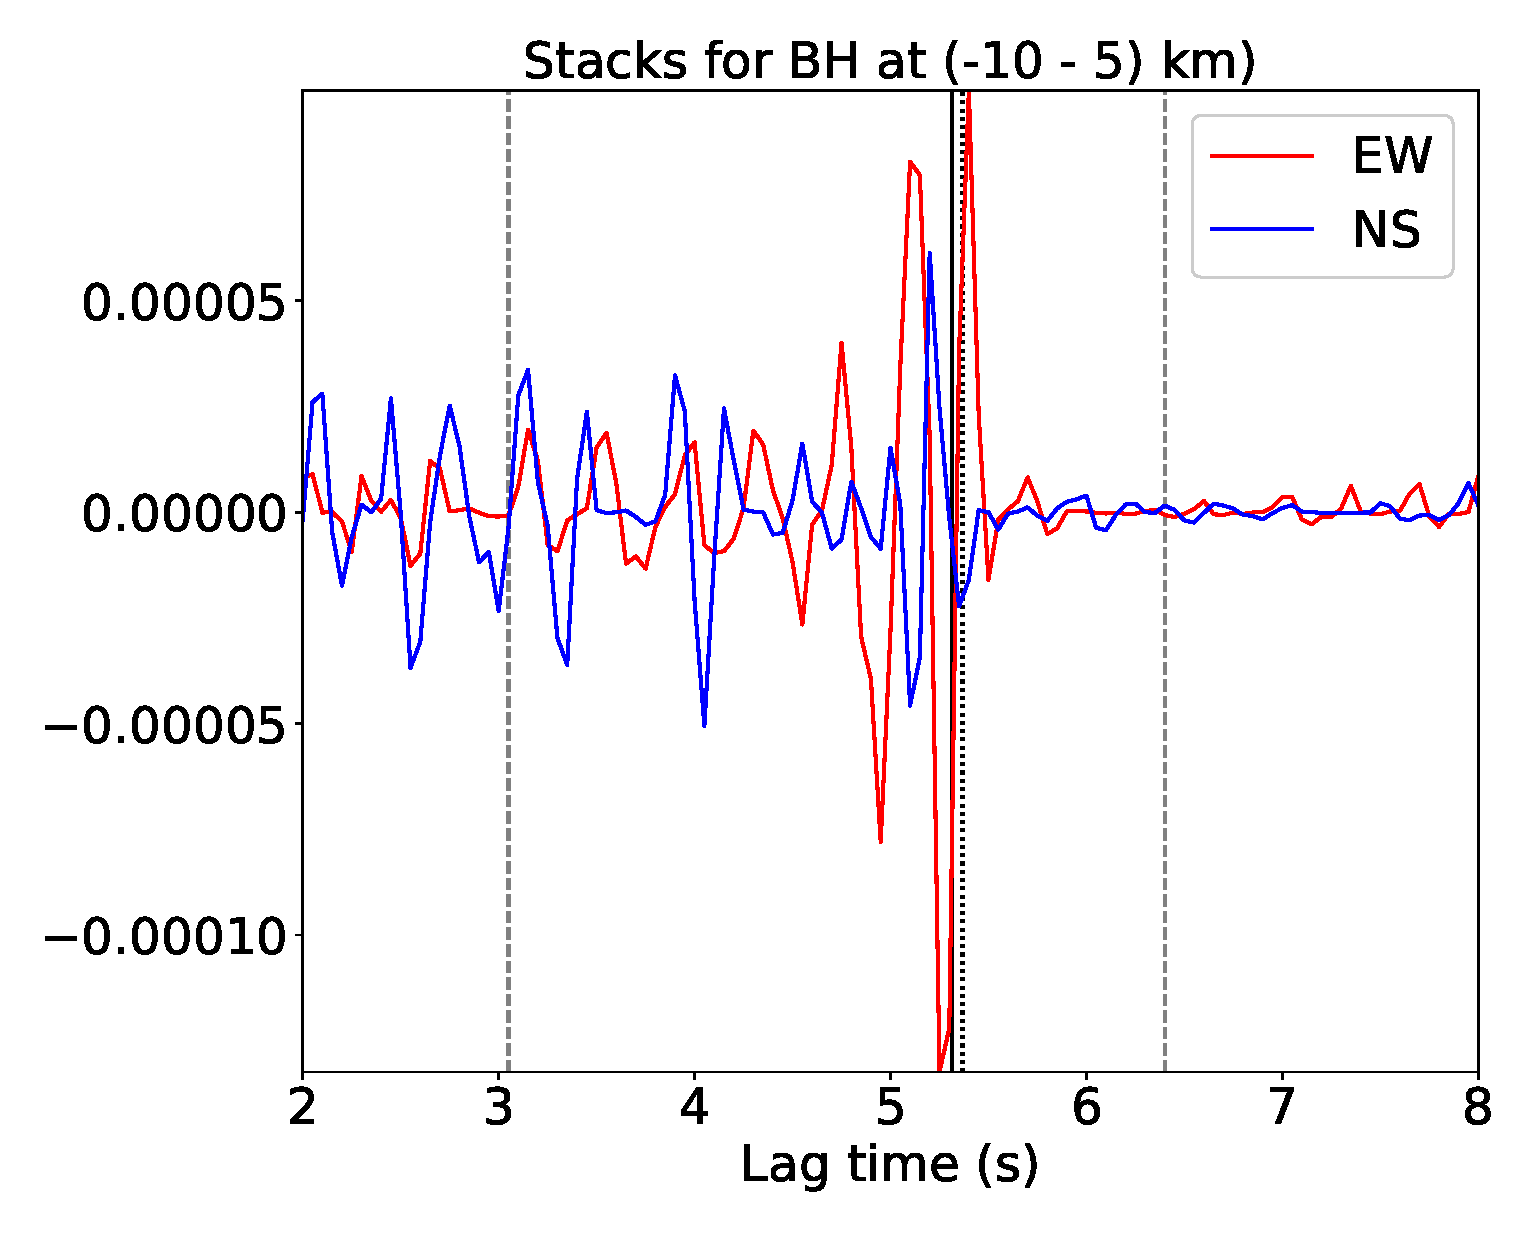
\includegraphics[width=\linewidth]{figures/intervals/BH_-10_005_stacks.eps}
\caption{See caption of Figure 1 for an explanation of this figure.}
\end{figure}

\begin{figure}[H]
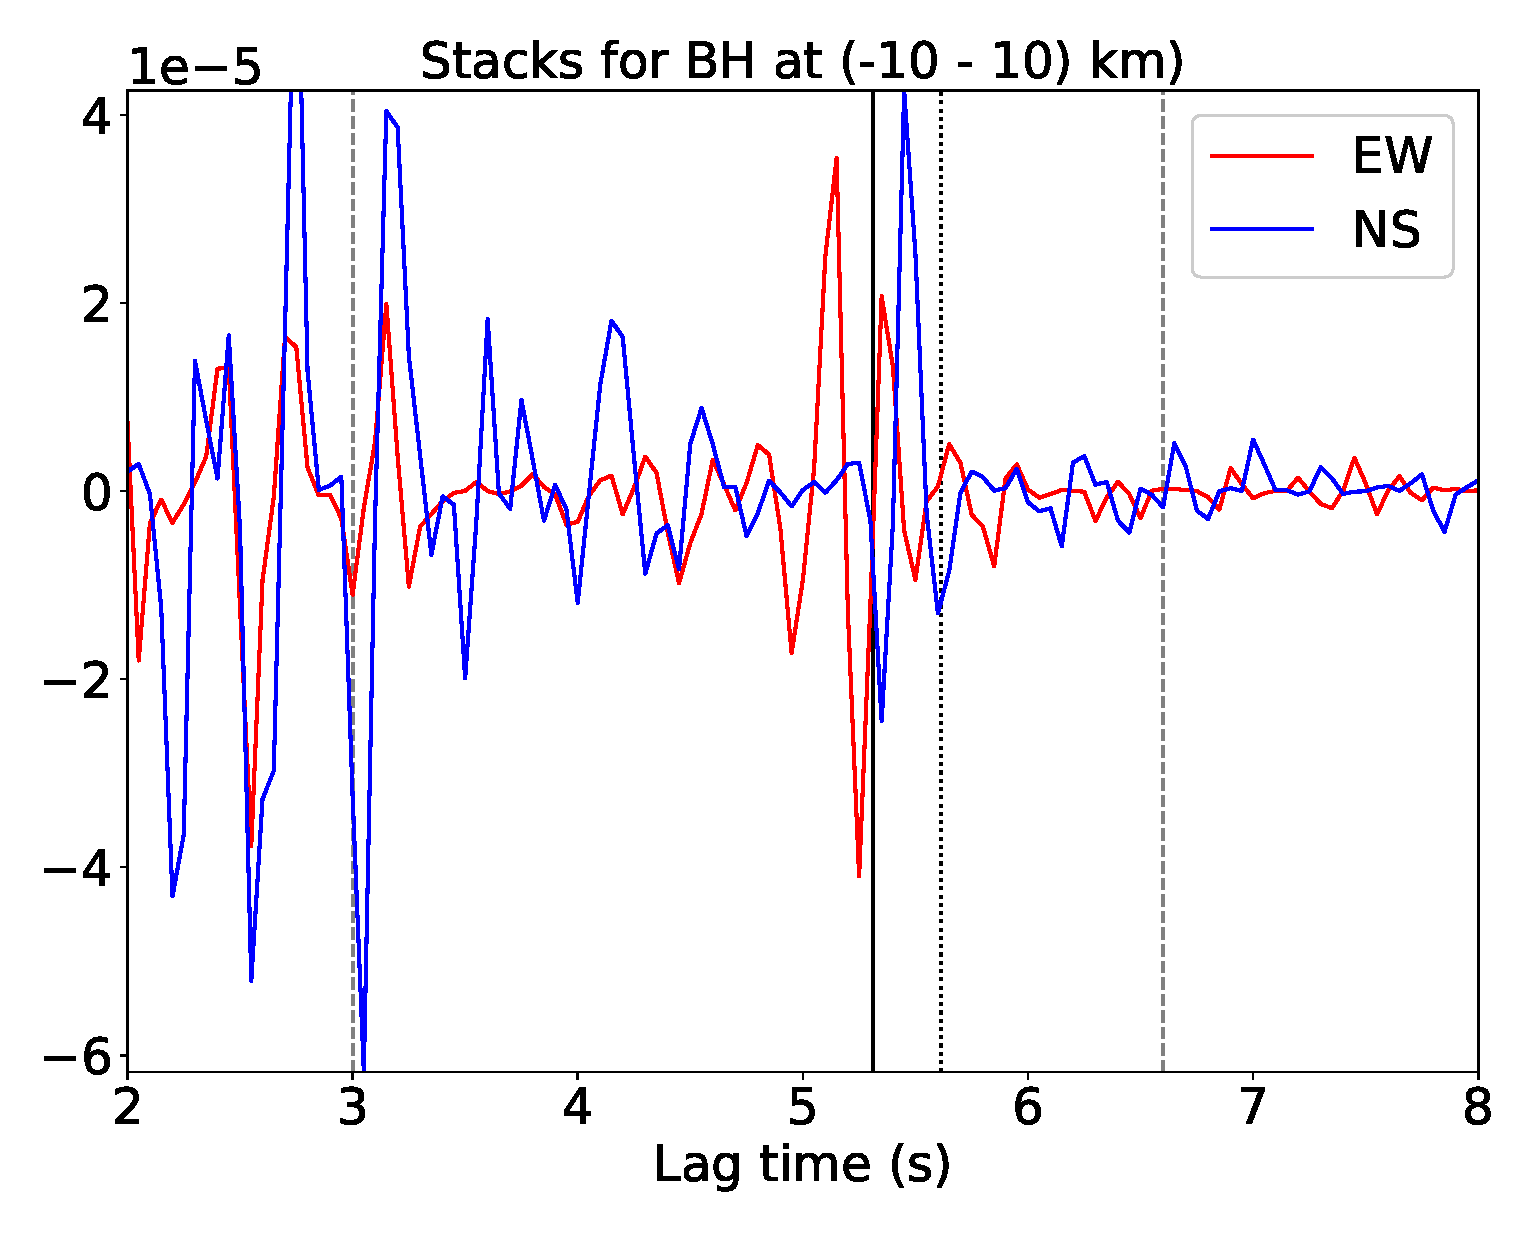
\includegraphics[width=\linewidth]{figures/intervals/BH_-10_010_stacks.eps}
\caption{See caption of Figure 1 for an explanation of this figure.}
\end{figure}

\begin{figure}[H]
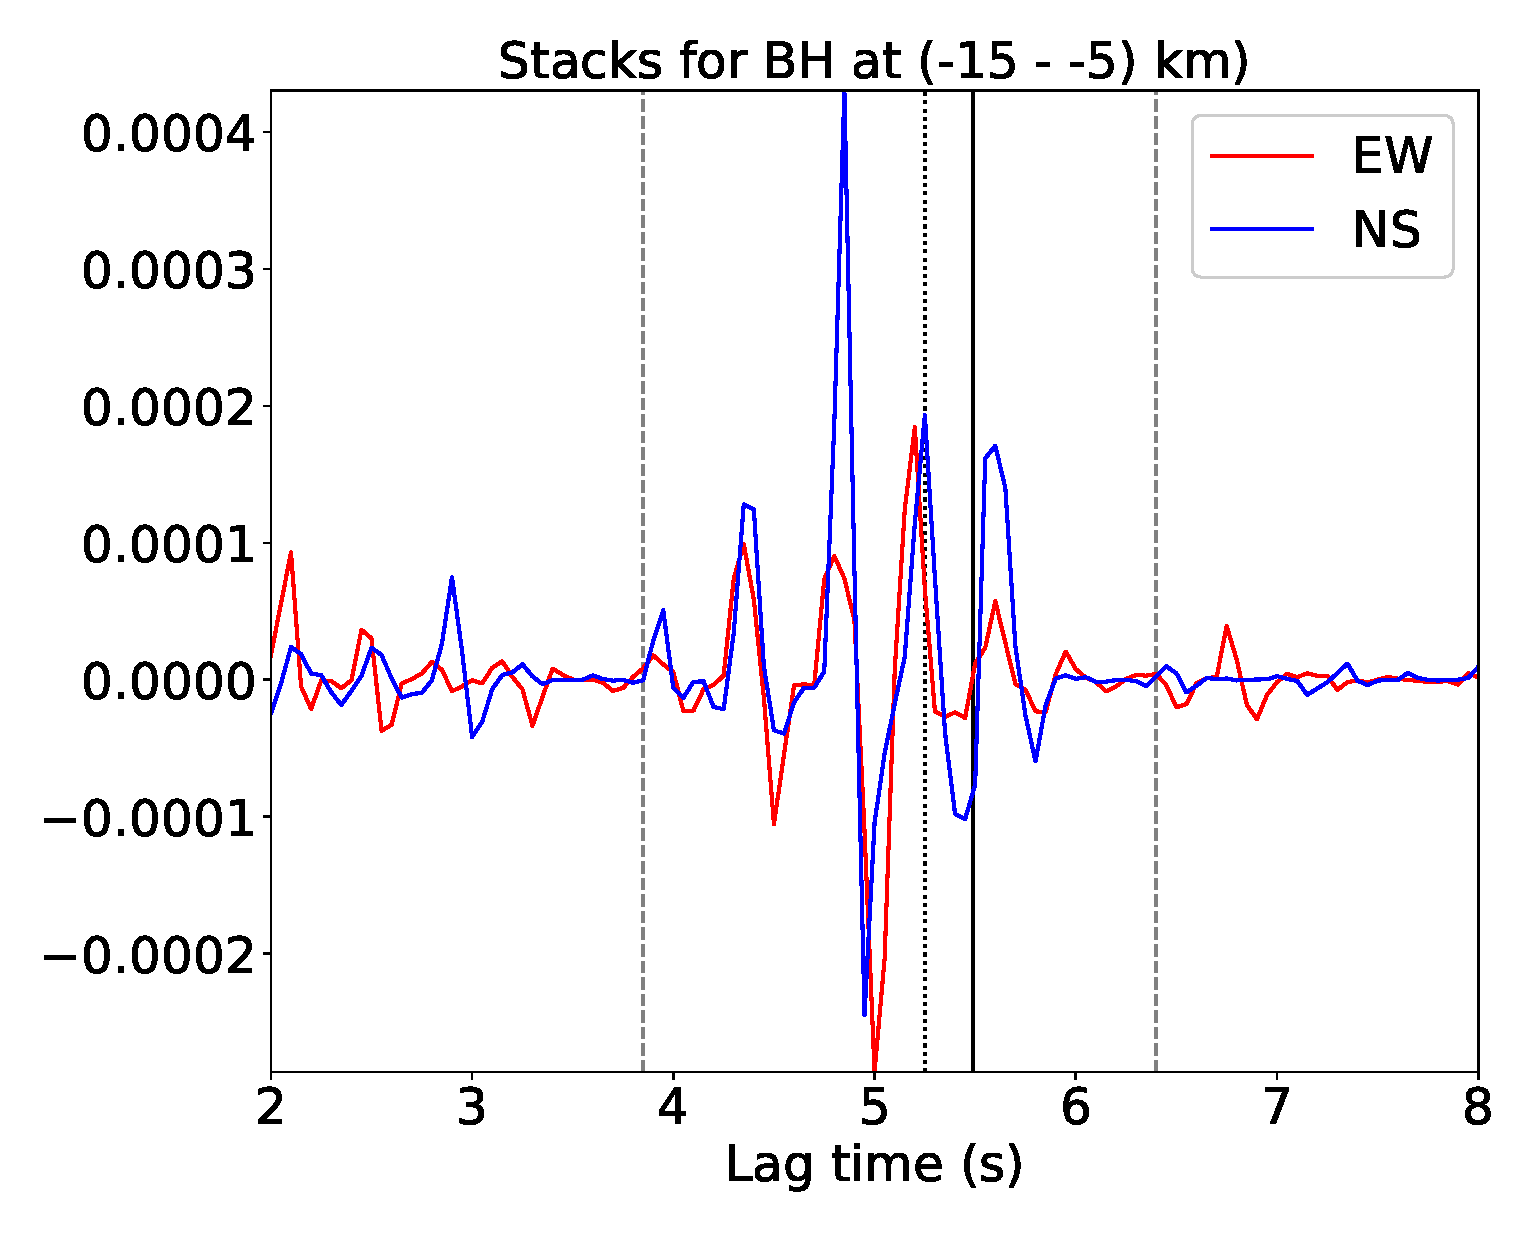
\includegraphics[width=\linewidth]{figures/intervals/BH_-15_-05_stacks.eps}
\caption{See caption of Figure 1 for an explanation of this figure.}
\end{figure}

\begin{figure}[H]
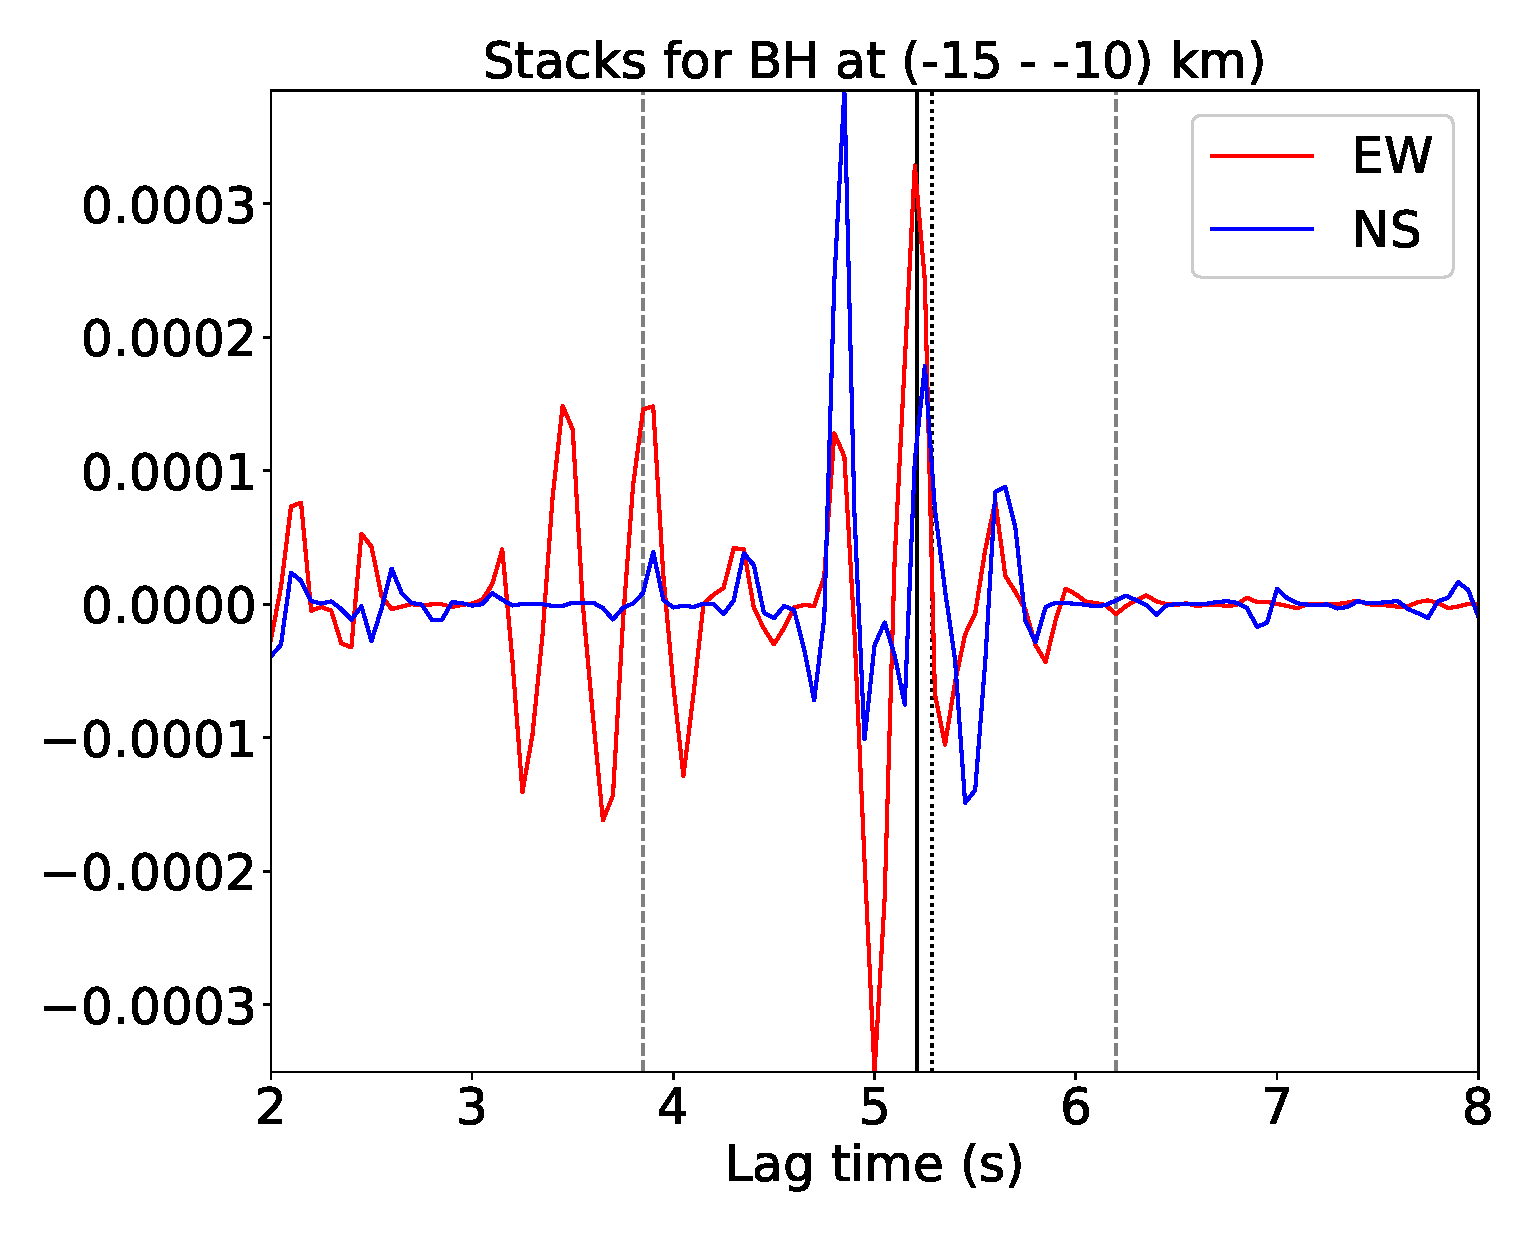
\includegraphics[width=\linewidth]{figures/intervals/BH_-15_-10_stacks.eps}
\caption{See caption of Figure 1 for an explanation of this figure.}
\end{figure}

\begin{figure}[H]
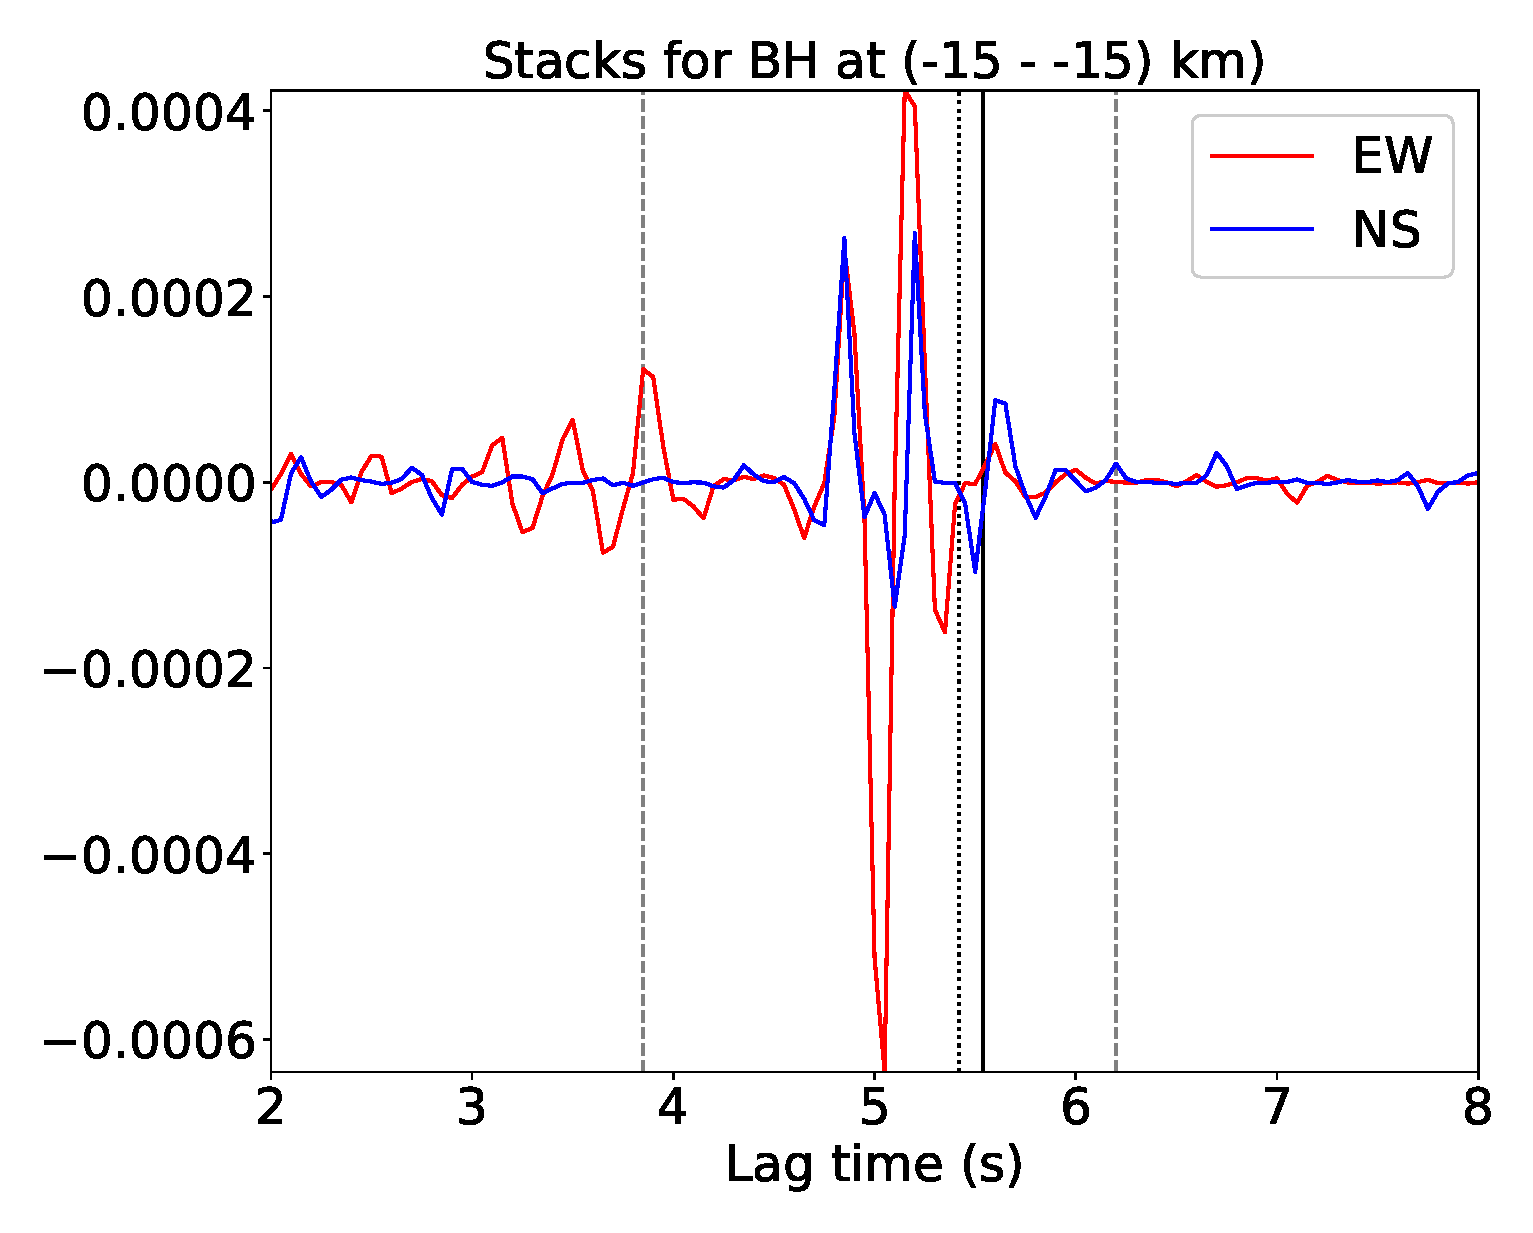
\includegraphics[width=\linewidth]{figures/intervals/BH_-15_-15_stacks.eps}
\caption{See caption of Figure 1 for an explanation of this figure.}
\end{figure}

\begin{figure}[H]
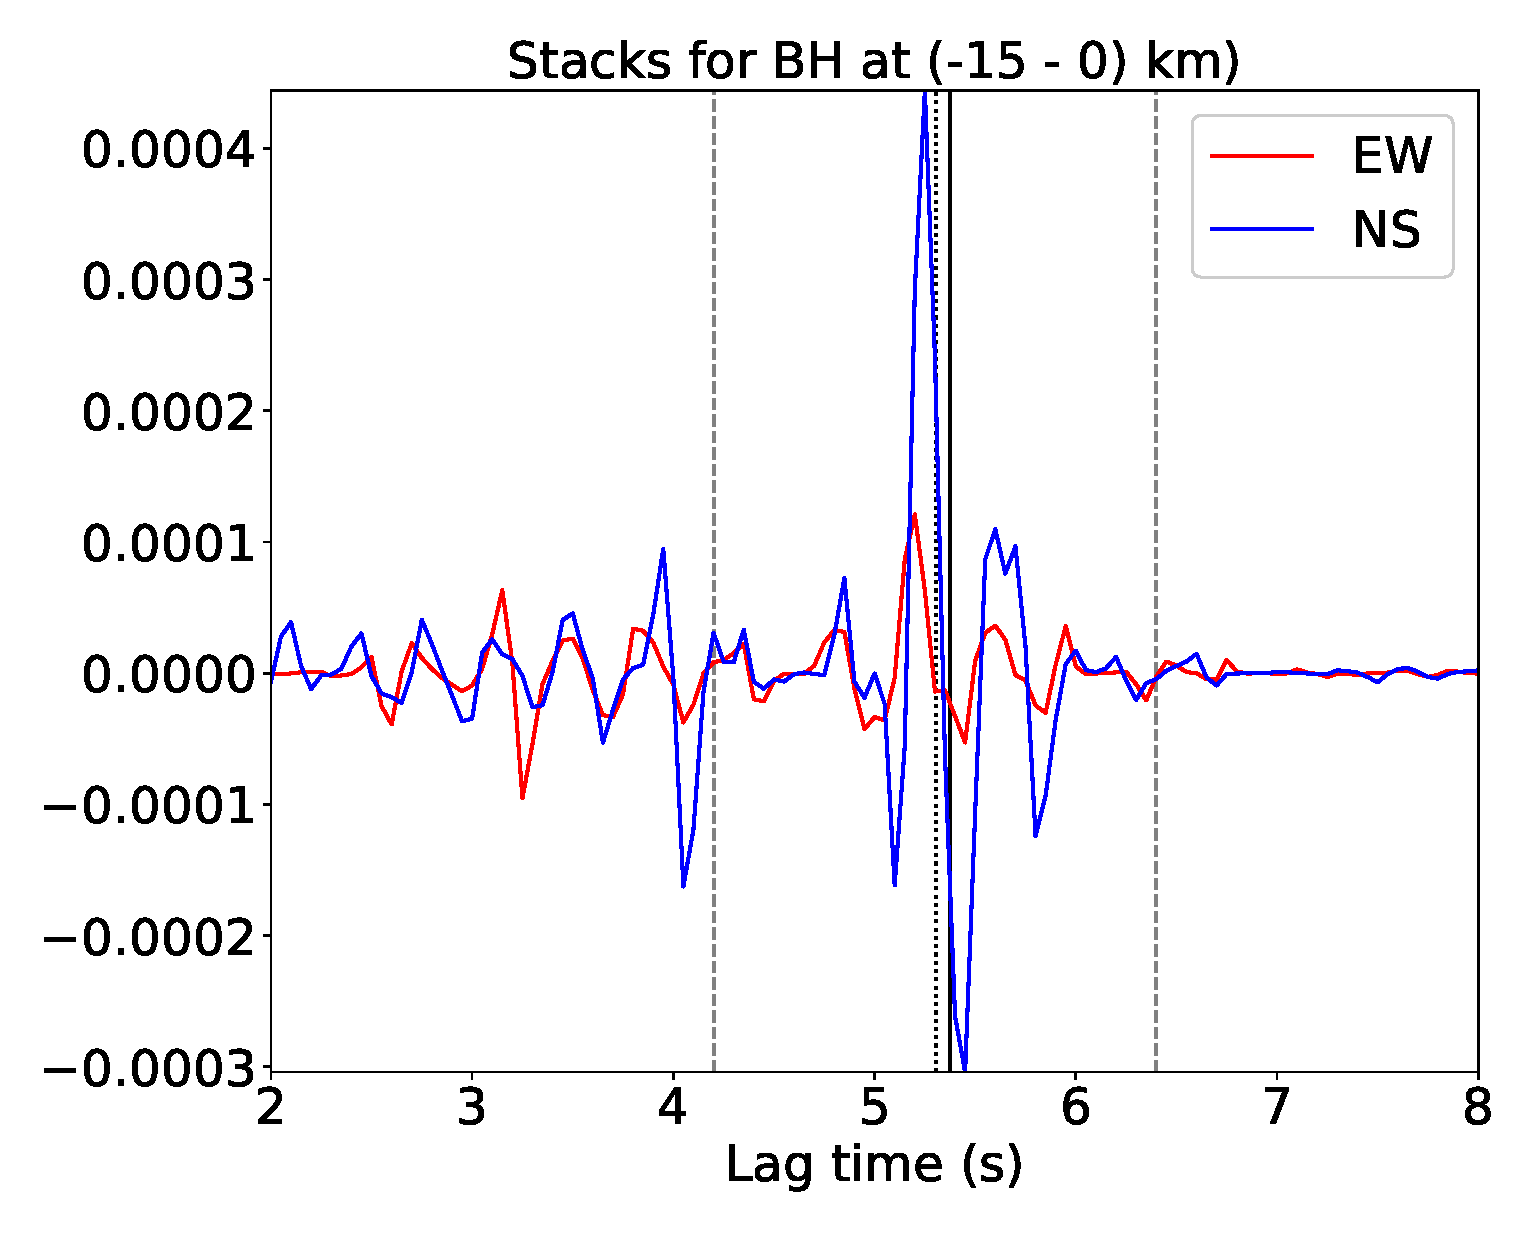
\includegraphics[width=\linewidth]{figures/intervals/BH_-15_000_stacks.eps}
\caption{See caption of Figure 1 for an explanation of this figure.}
\end{figure}

\begin{figure}[H]
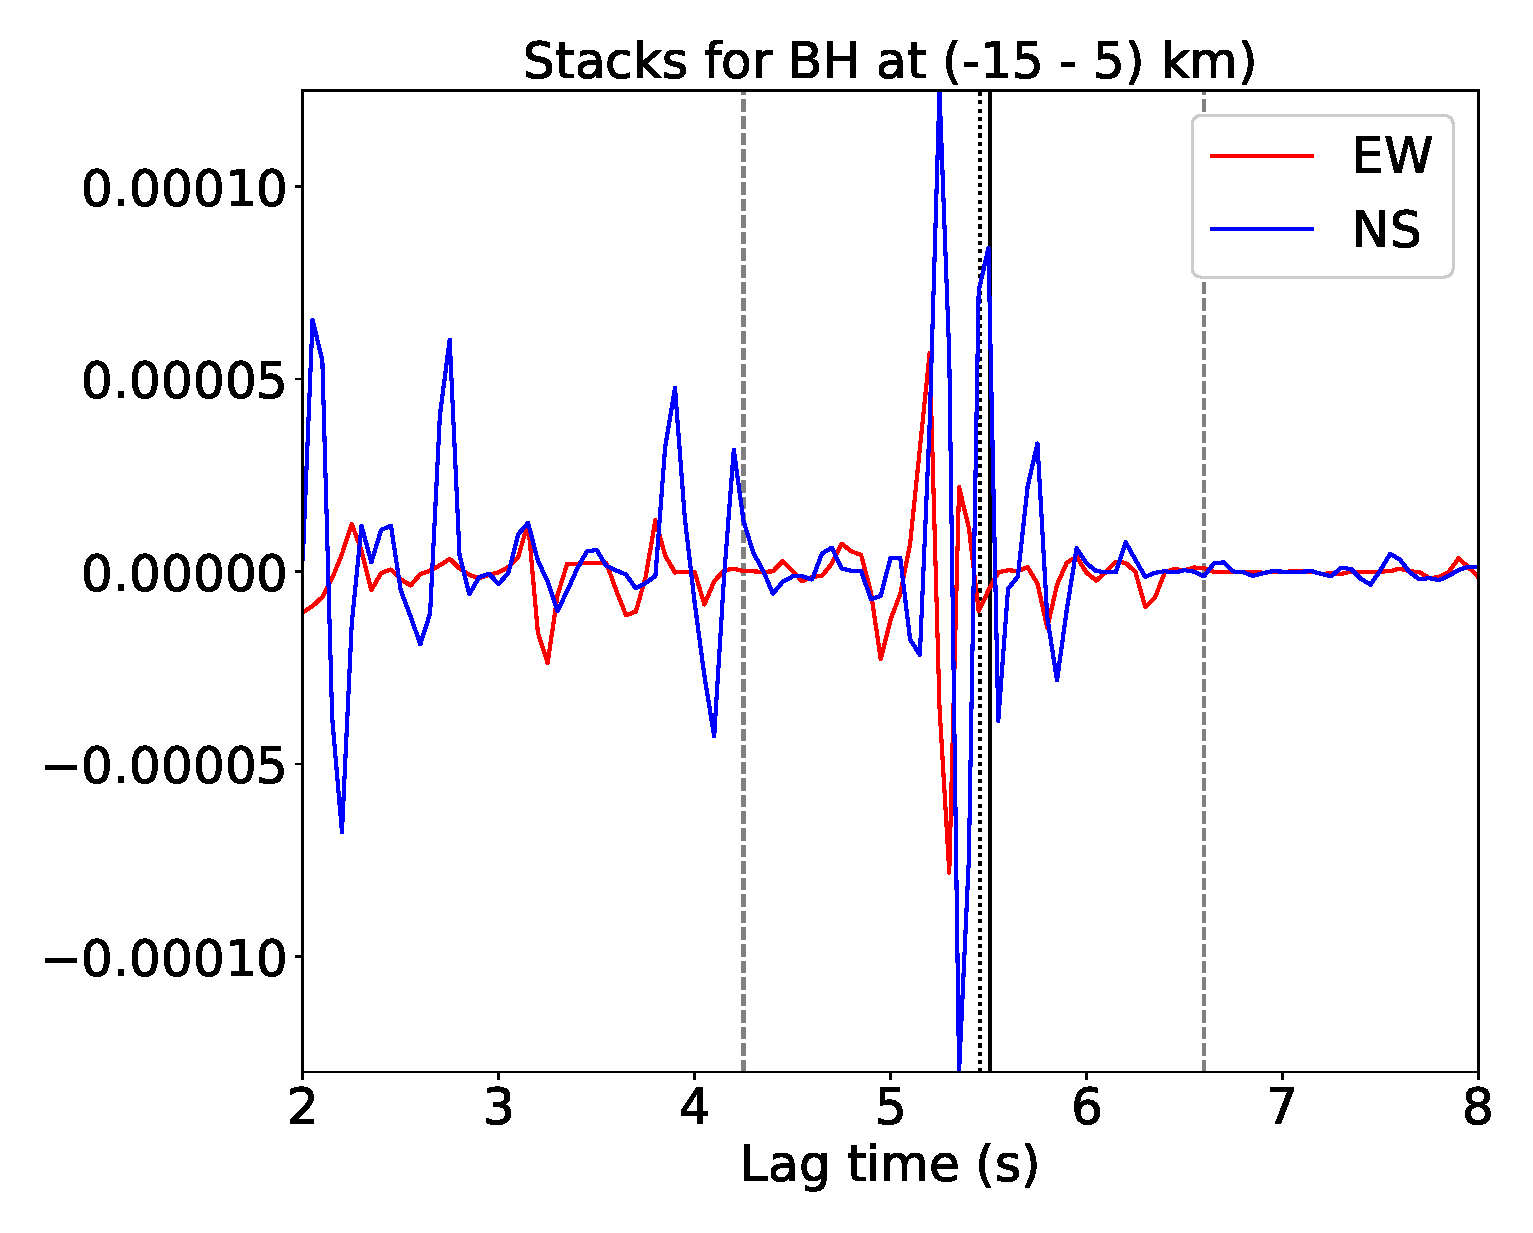
\includegraphics[width=\linewidth]{figures/intervals/BH_-15_005_stacks.eps}
\caption{See caption of Figure 1 for an explanation of this figure.}
\end{figure}

\begin{figure}[H]
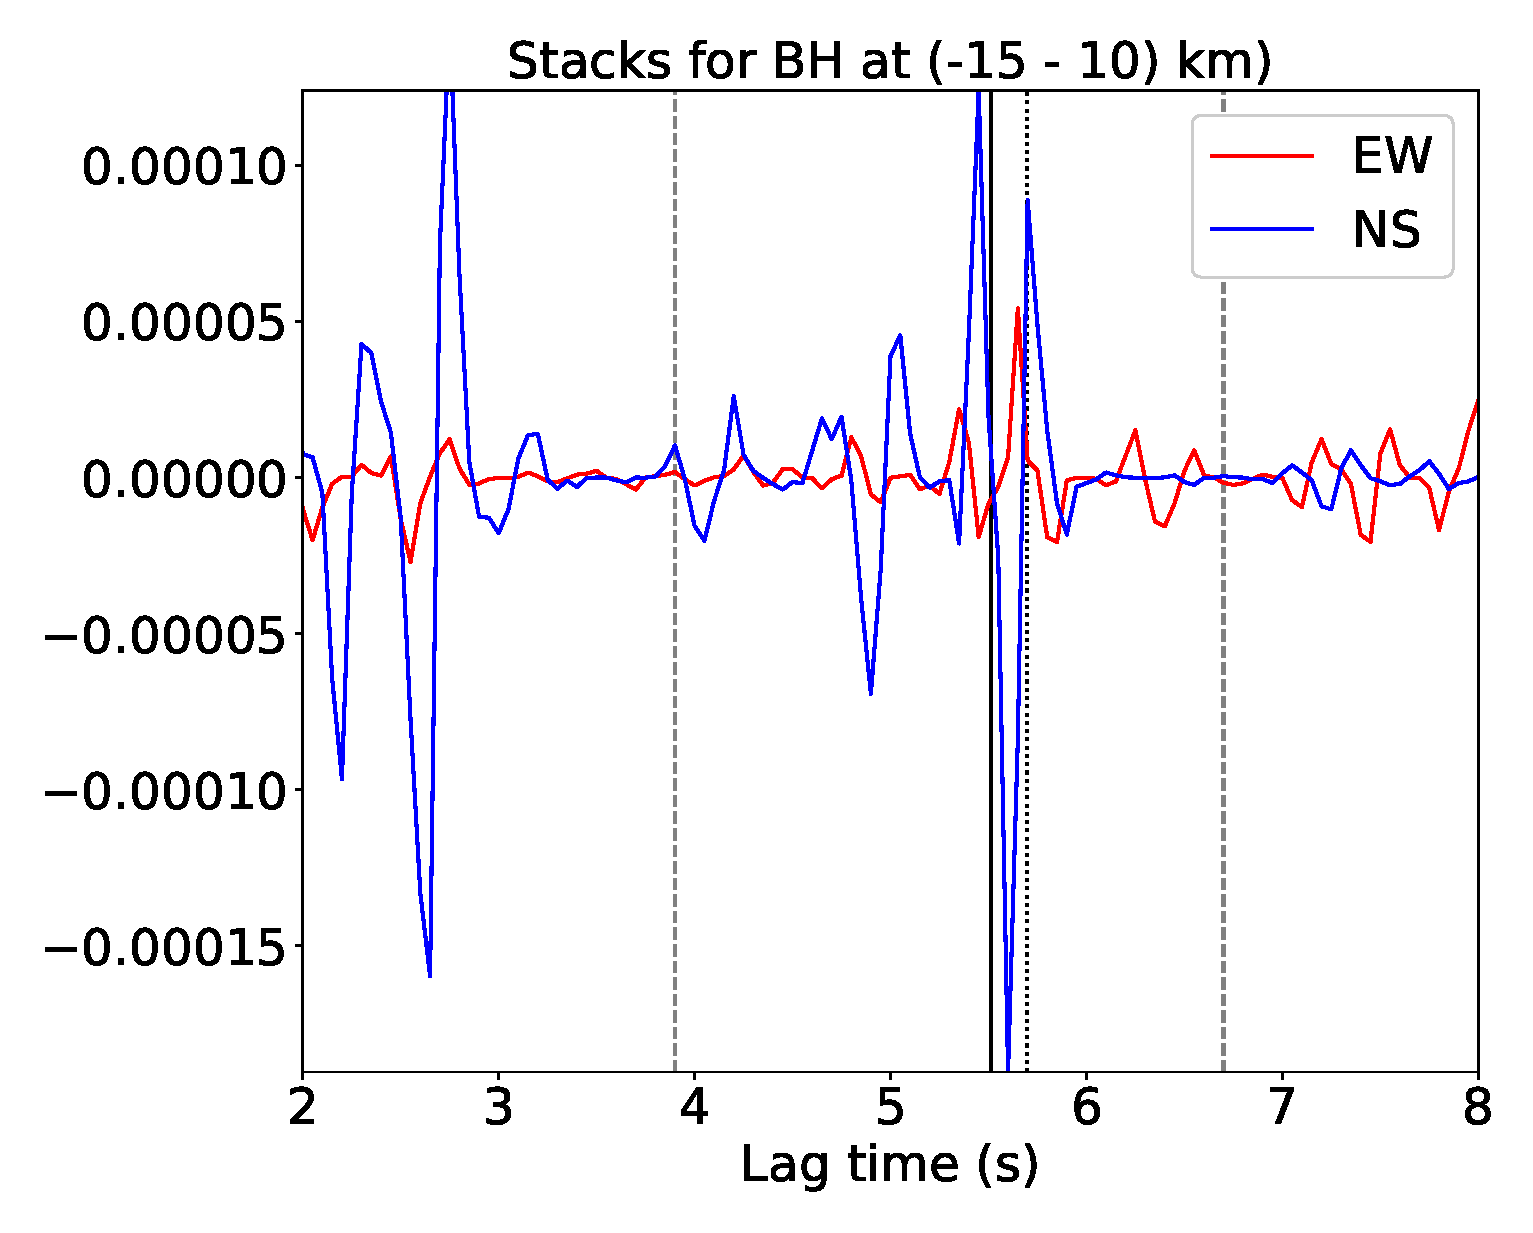
\includegraphics[width=\linewidth]{figures/intervals/BH_-15_010_stacks.eps}
\caption{See caption of Figure 1 for an explanation of this figure.}
\end{figure}

\begin{figure}[H]
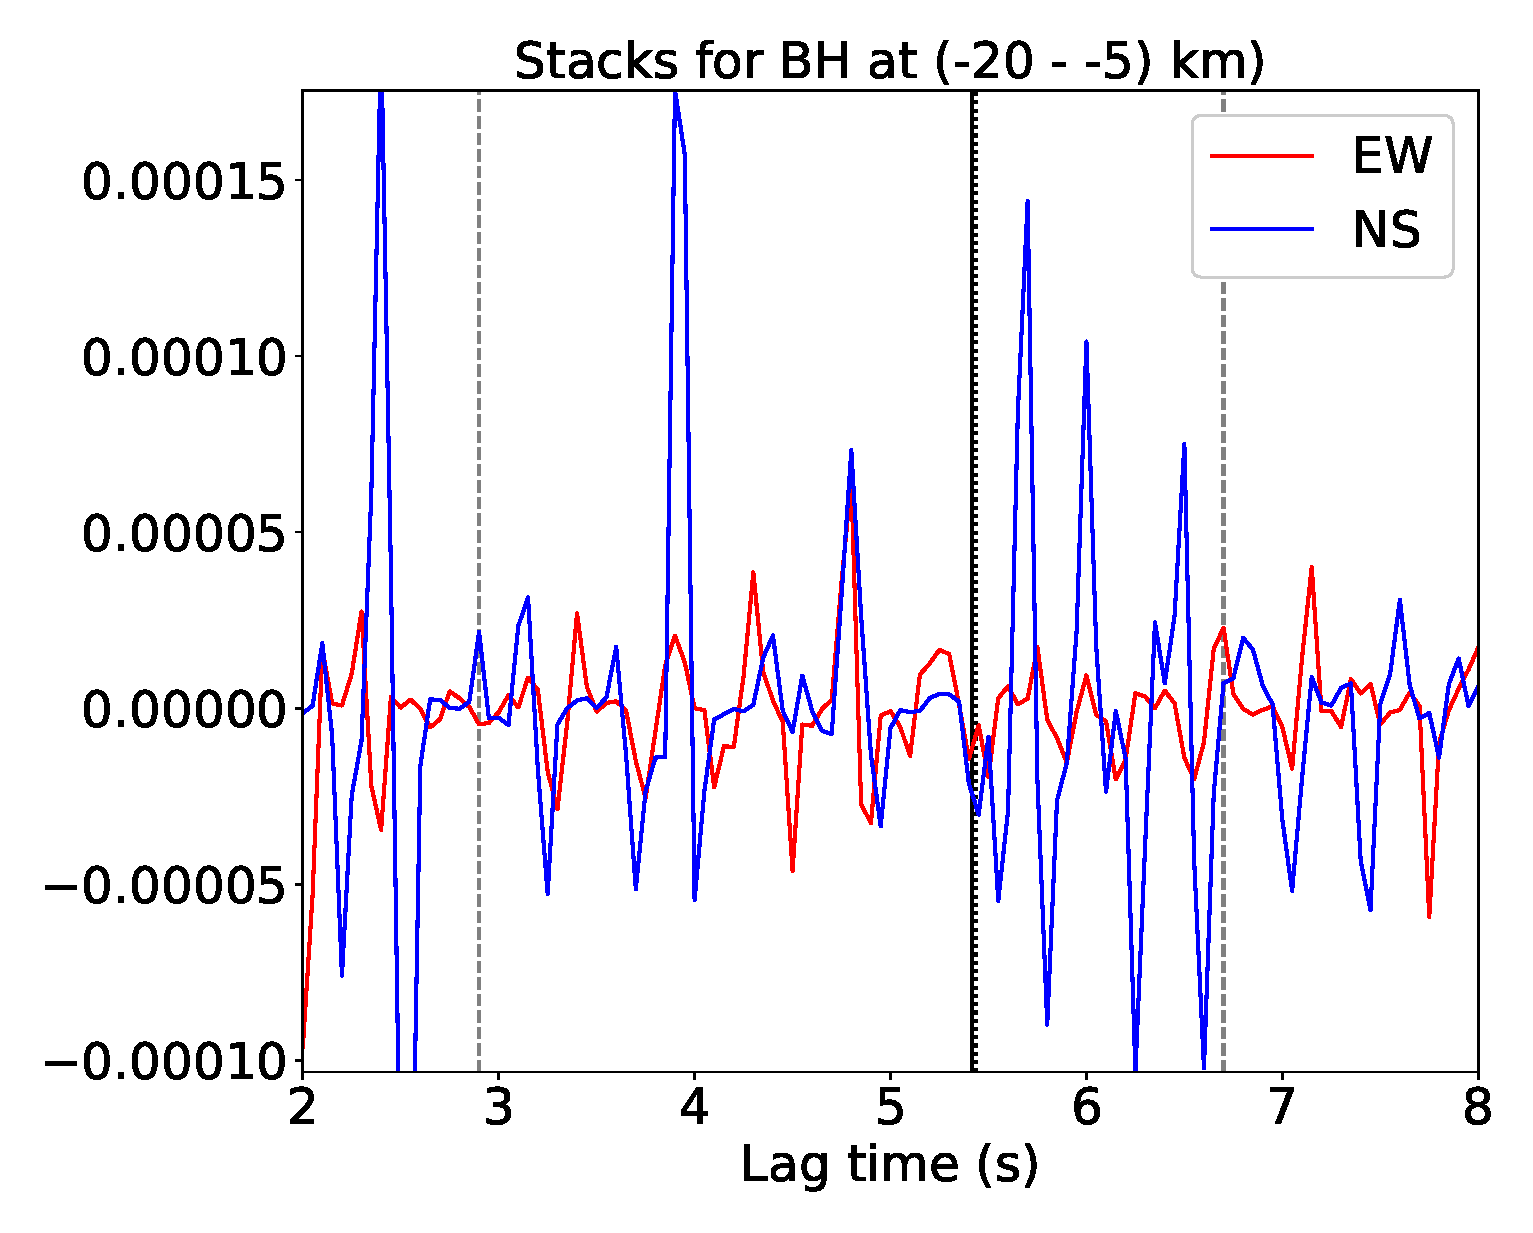
\includegraphics[width=\linewidth]{figures/intervals/BH_-20_-05_stacks.eps}
\caption{See caption of Figure 1 for an explanation of this figure.}
\end{figure}

\begin{figure}[H]
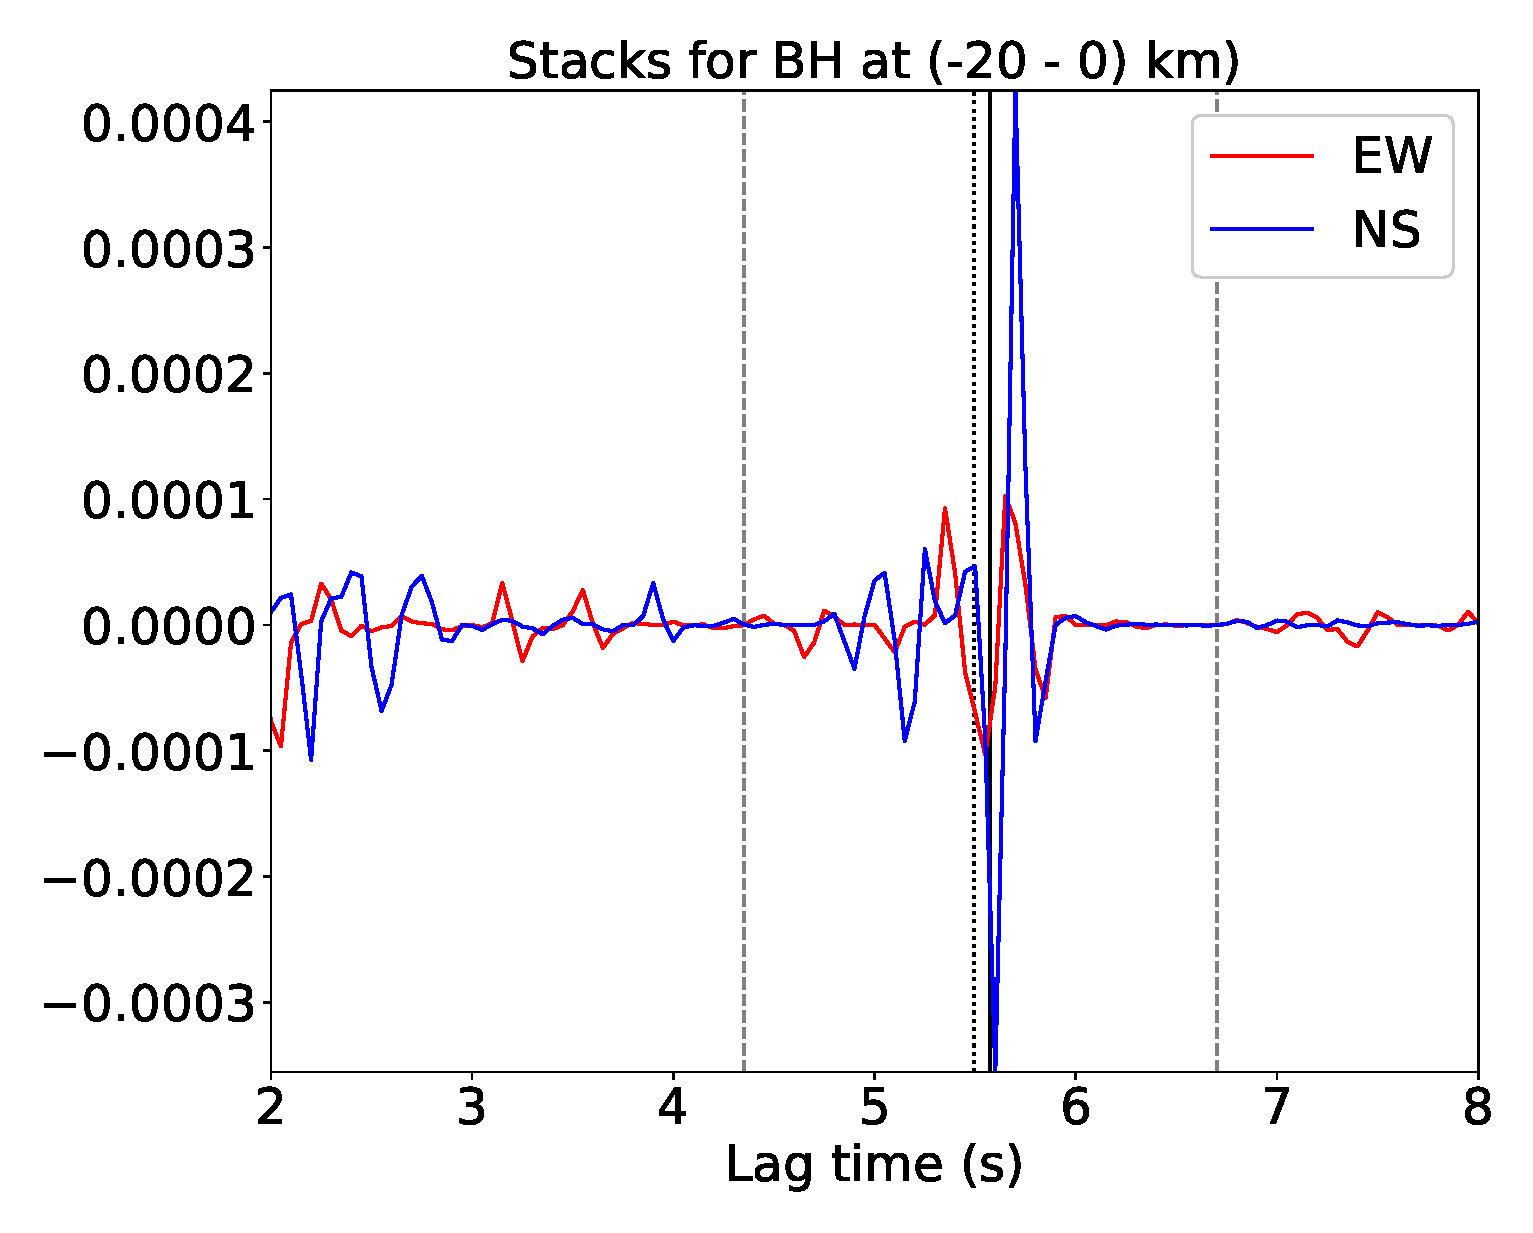
\includegraphics[width=\linewidth]{figures/intervals/BH_-20_000_stacks.eps}
\caption{See caption of Figure 1 for an explanation of this figure.}
\end{figure}

\begin{figure}[H]
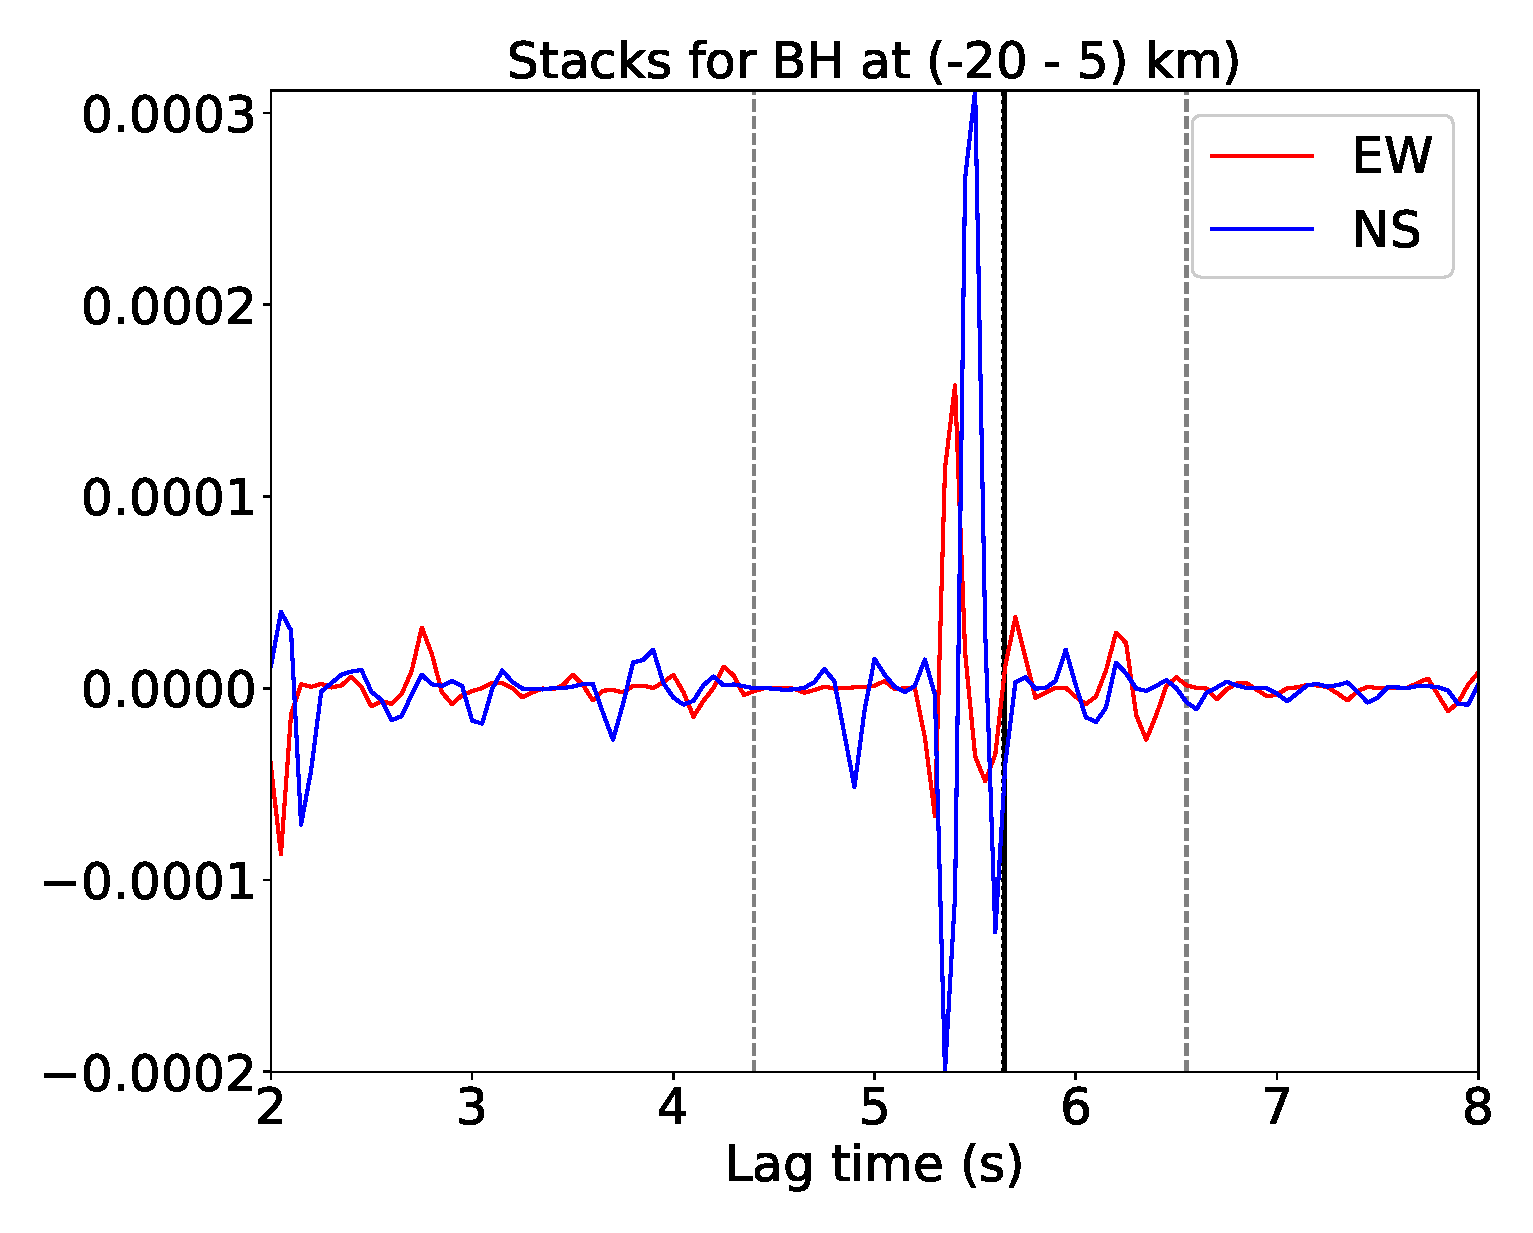
\includegraphics[width=\linewidth]{figures/intervals/BH_-20_005_stacks.eps}
\caption{See caption of Figure 1 for an explanation of this figure.}
\end{figure}

\begin{figure}[H]
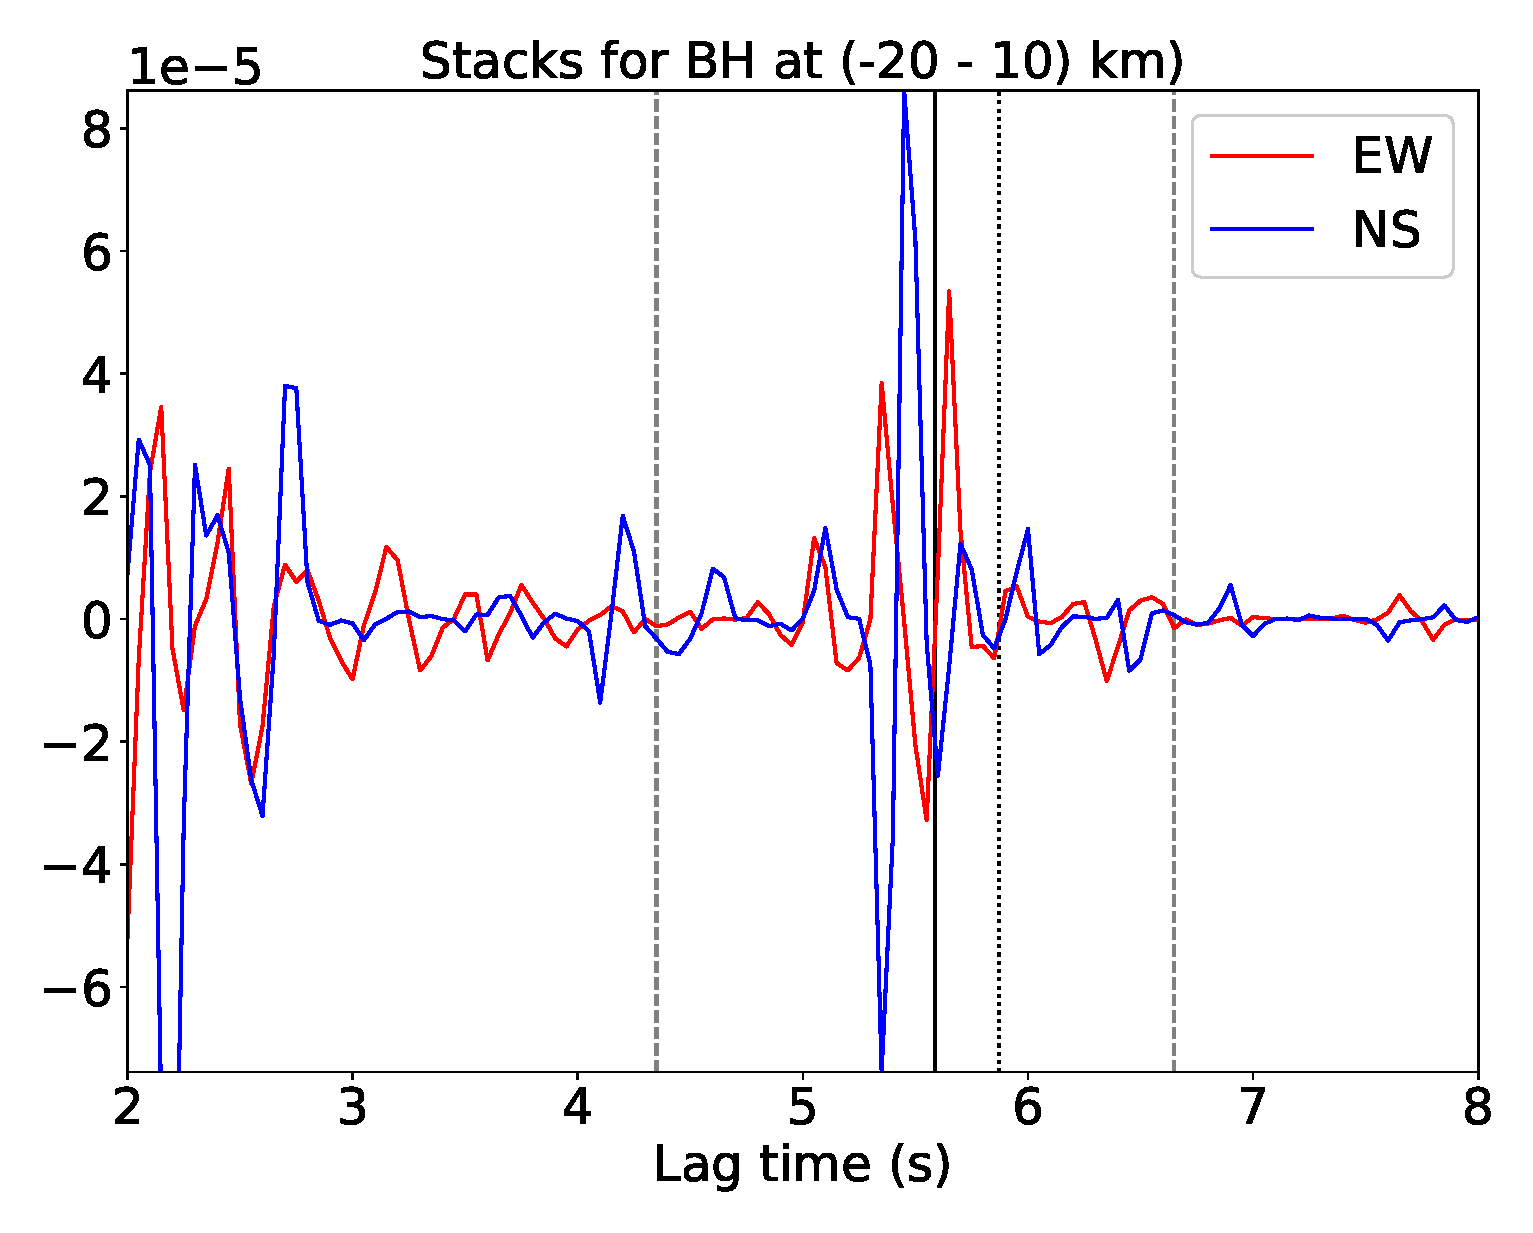
\includegraphics[width=\linewidth]{figures/intervals/BH_-20_010_stacks.eps}
\caption{See caption of Figure 1 for an explanation of this figure.}
\end{figure}

\begin{figure}[H]
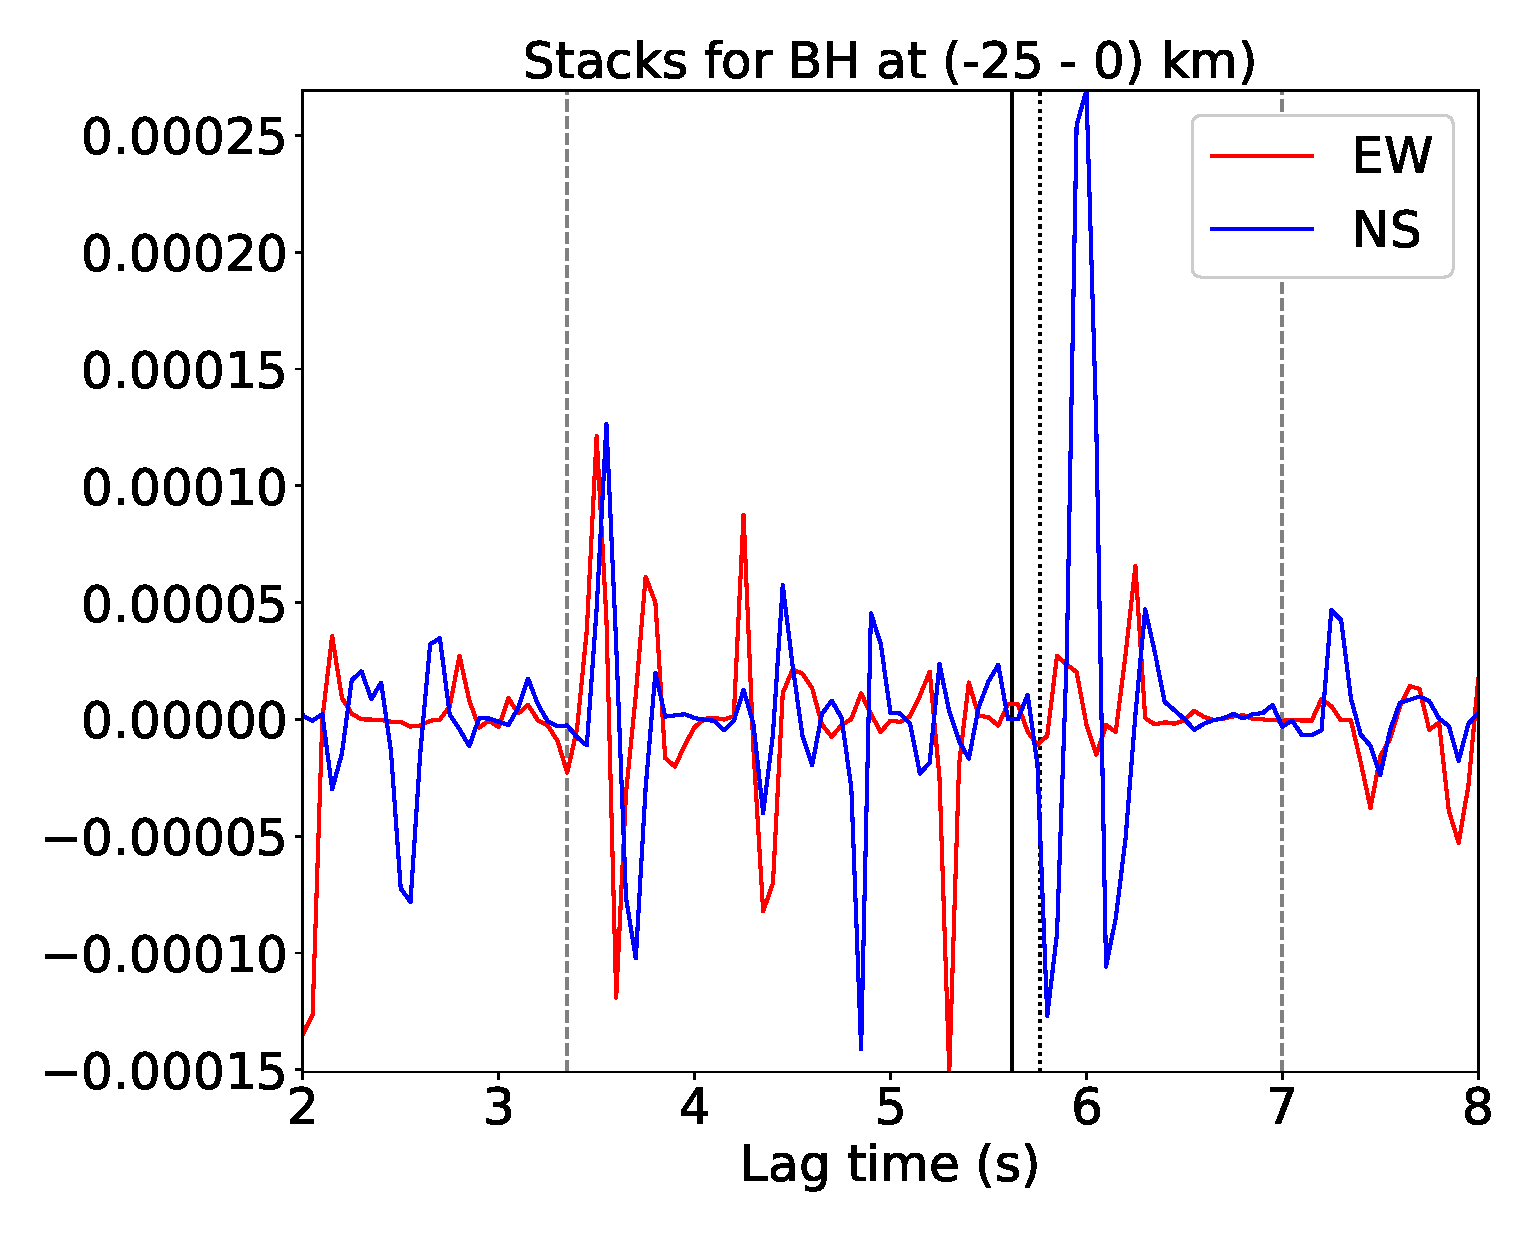
\includegraphics[width=\linewidth]{figures/intervals/BH_-25_000_stacks.eps}
\caption{See caption of Figure 1 for an explanation of this figure.}
\end{figure}

\begin{figure}[H]
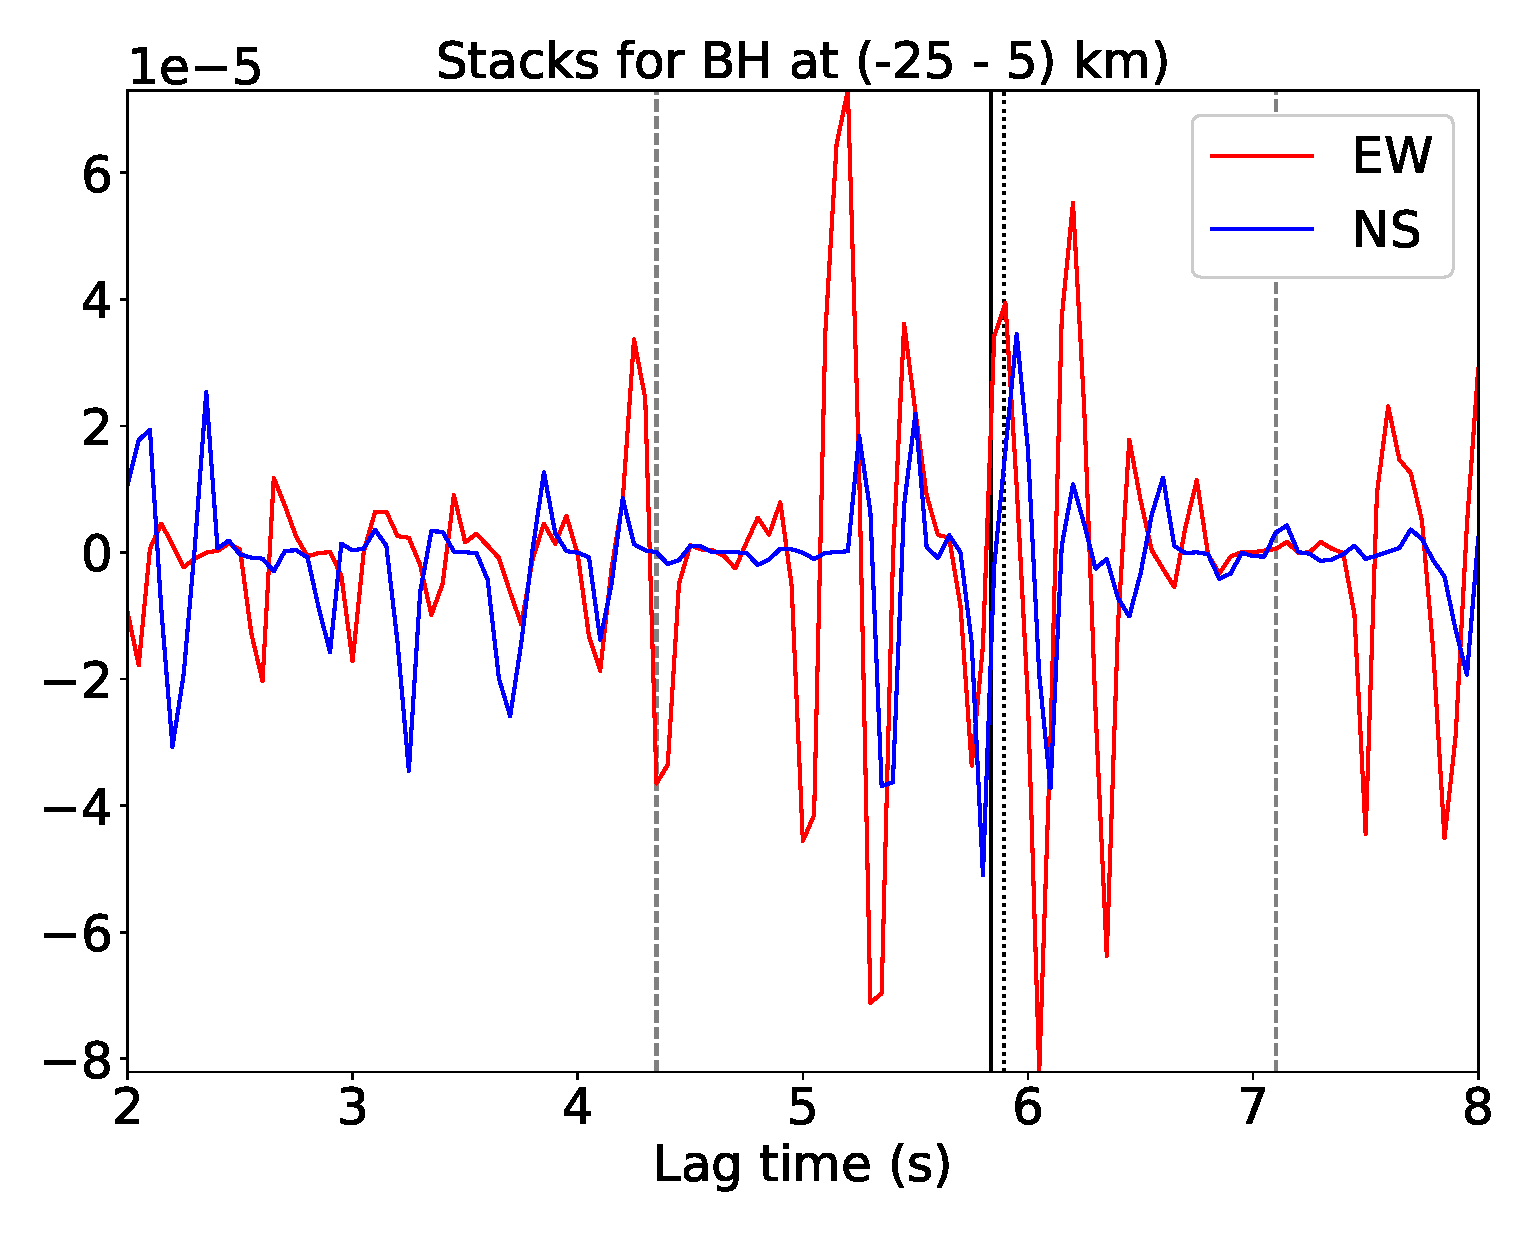
\includegraphics[width=\linewidth]{figures/intervals/BH_-25_005_stacks.eps}
\caption{See caption of Figure 1 for an explanation of this figure.}
\end{figure}

\begin{figure}[H]
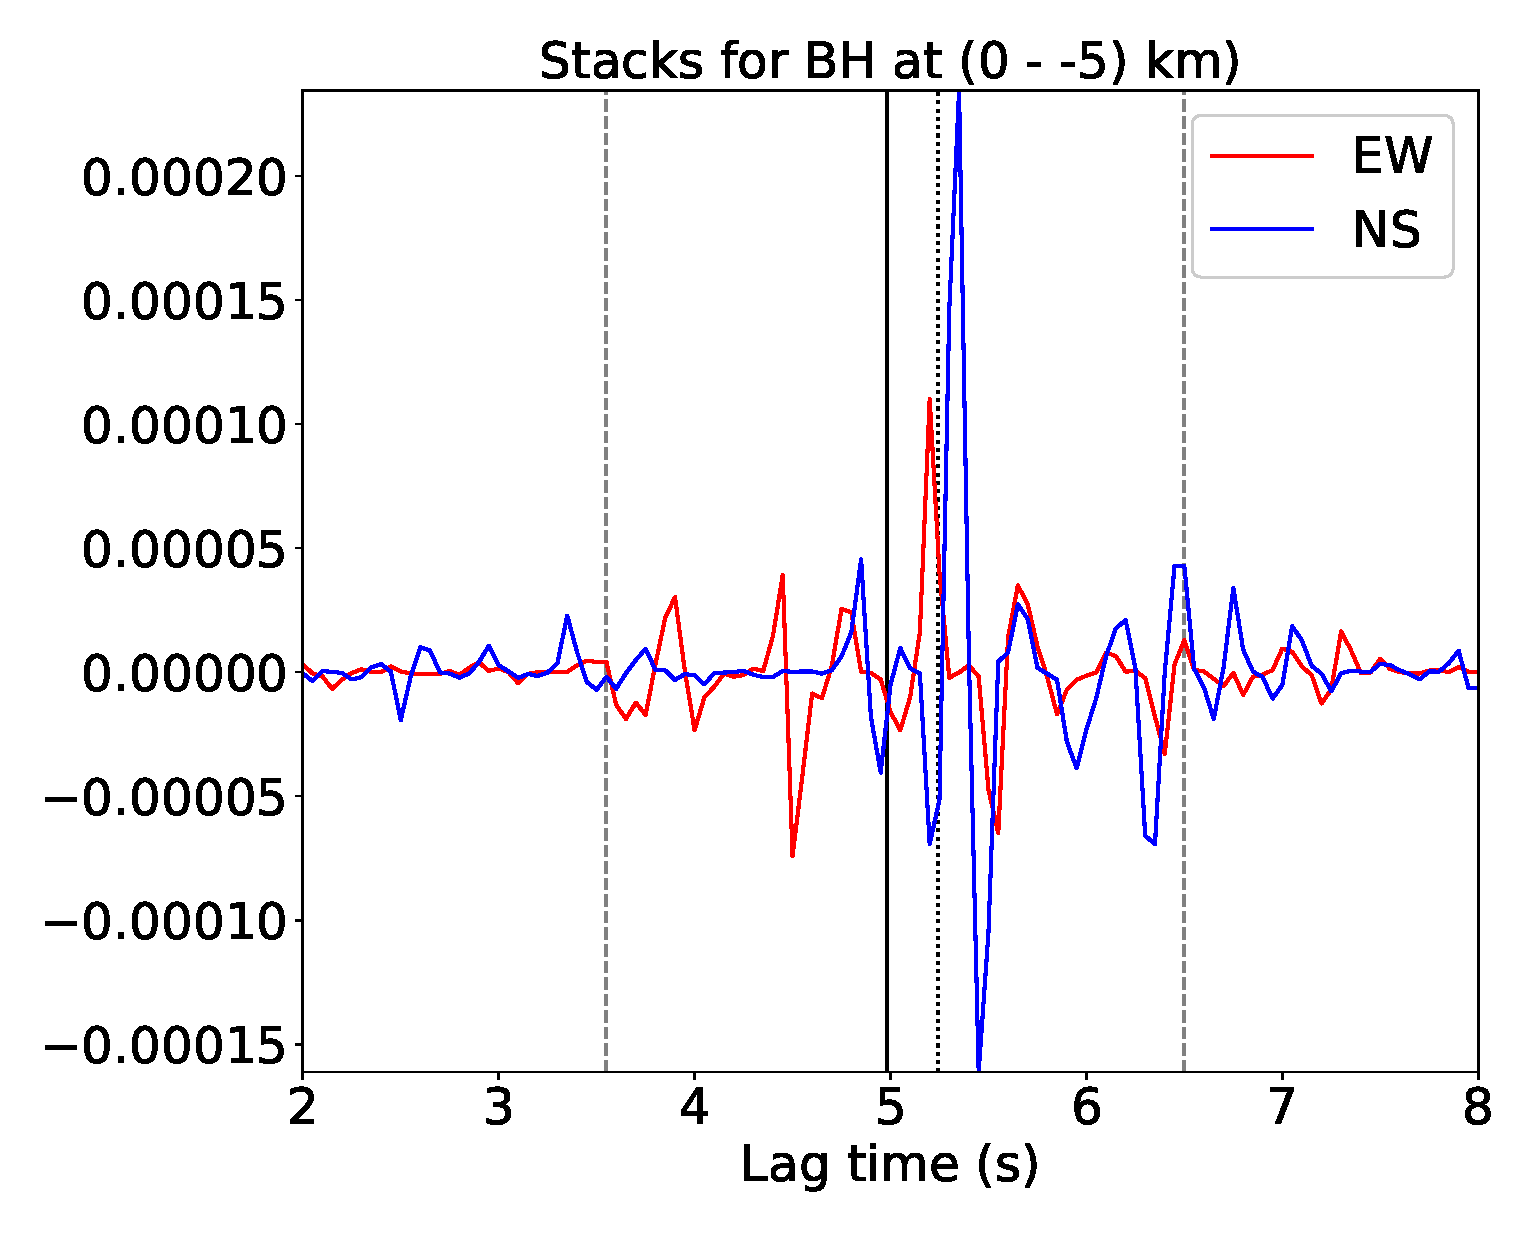
\includegraphics[width=\linewidth]{figures/intervals/BH_000_-05_stacks.eps}
\caption{See caption of Figure 1 for an explanation of this figure.}
\end{figure}

\begin{figure}[H]
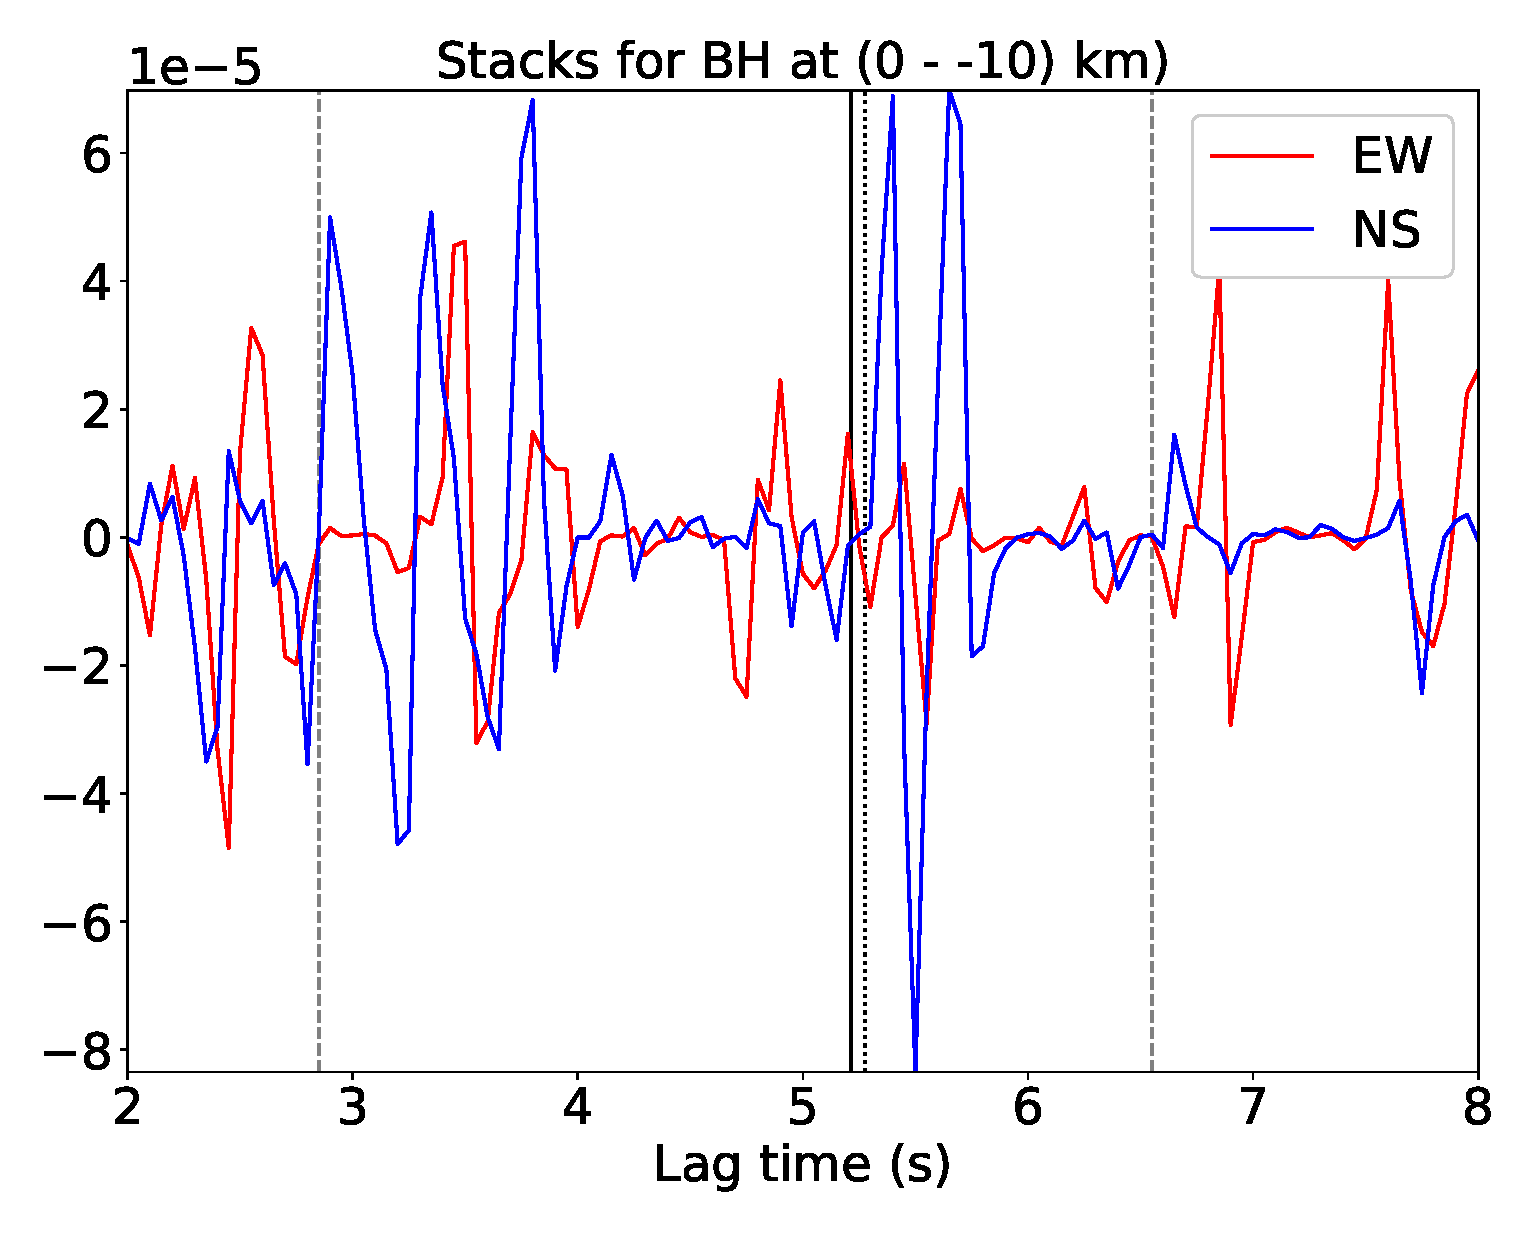
\includegraphics[width=\linewidth]{figures/intervals/BH_000_-10_stacks.eps}
\caption{See caption of Figure 1 for an explanation of this figure.}
\end{figure}

\begin{figure}[H]
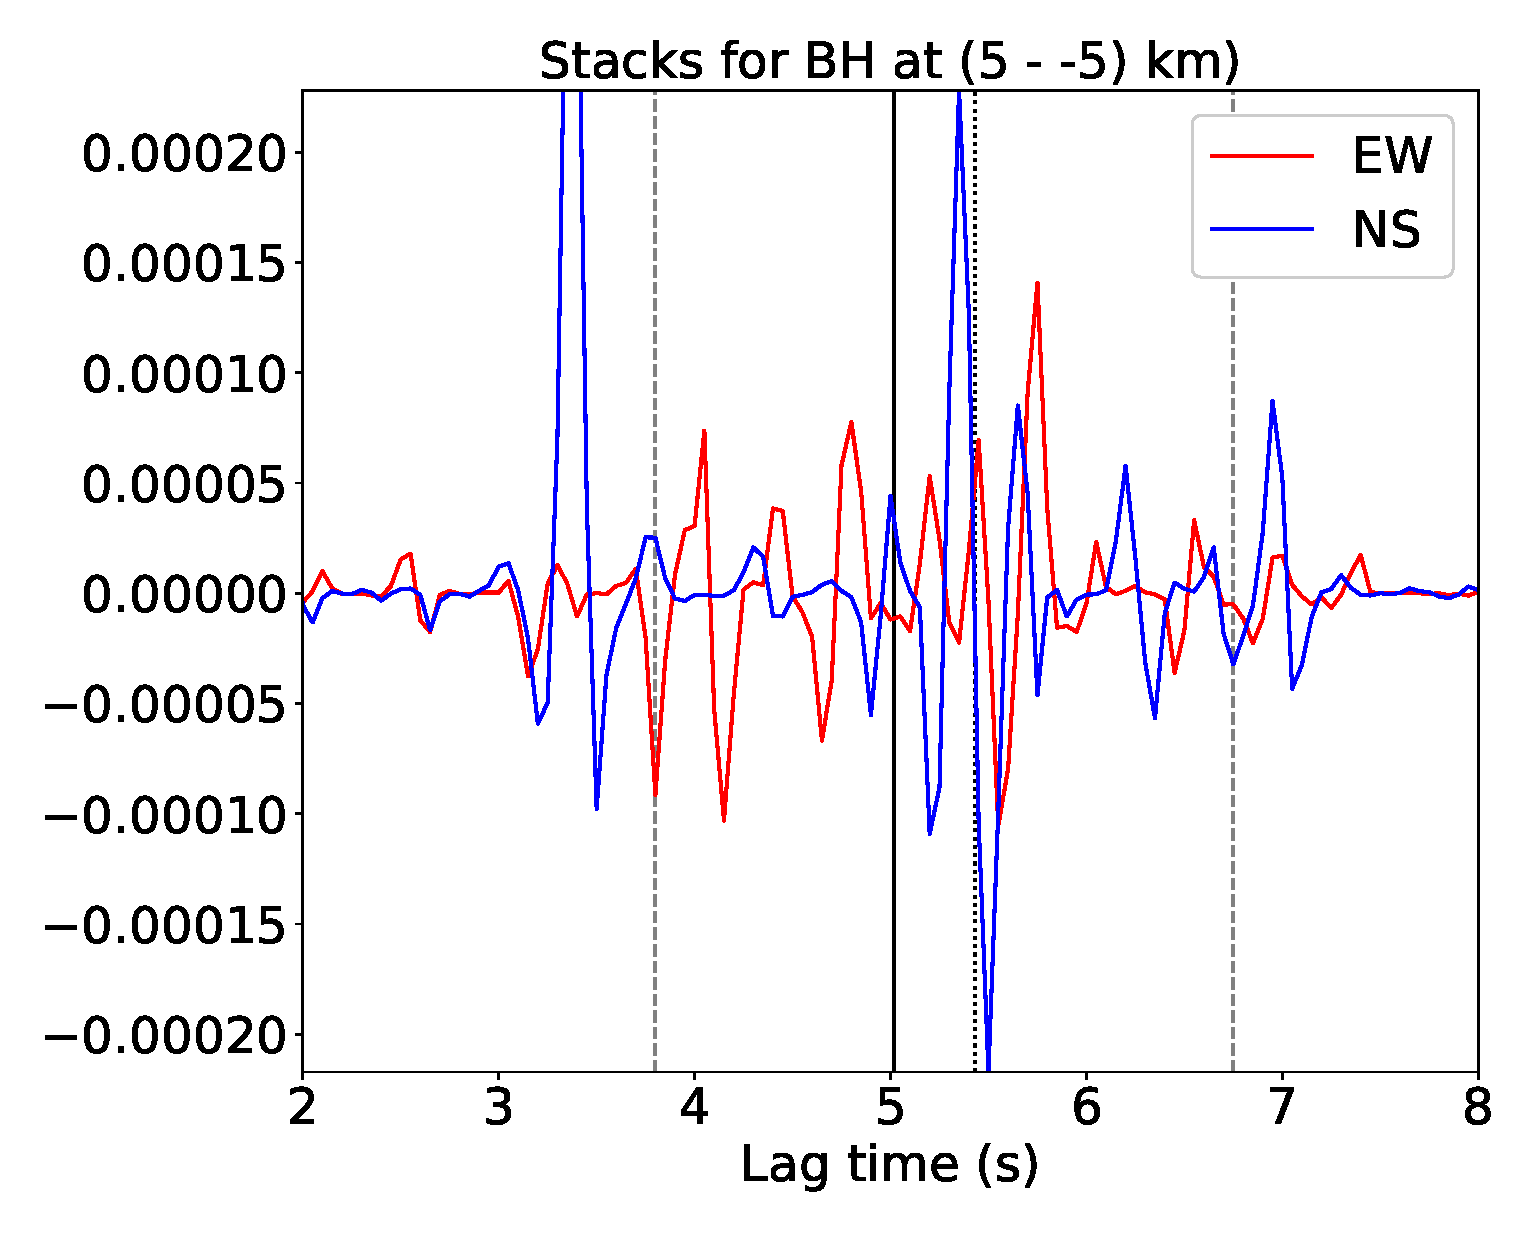
\includegraphics[width=\linewidth]{figures/intervals/BH_005_-05_stacks.eps}
\caption{See caption of Figure 1 for an explanation of this figure.}
\end{figure}

\begin{figure}[H]
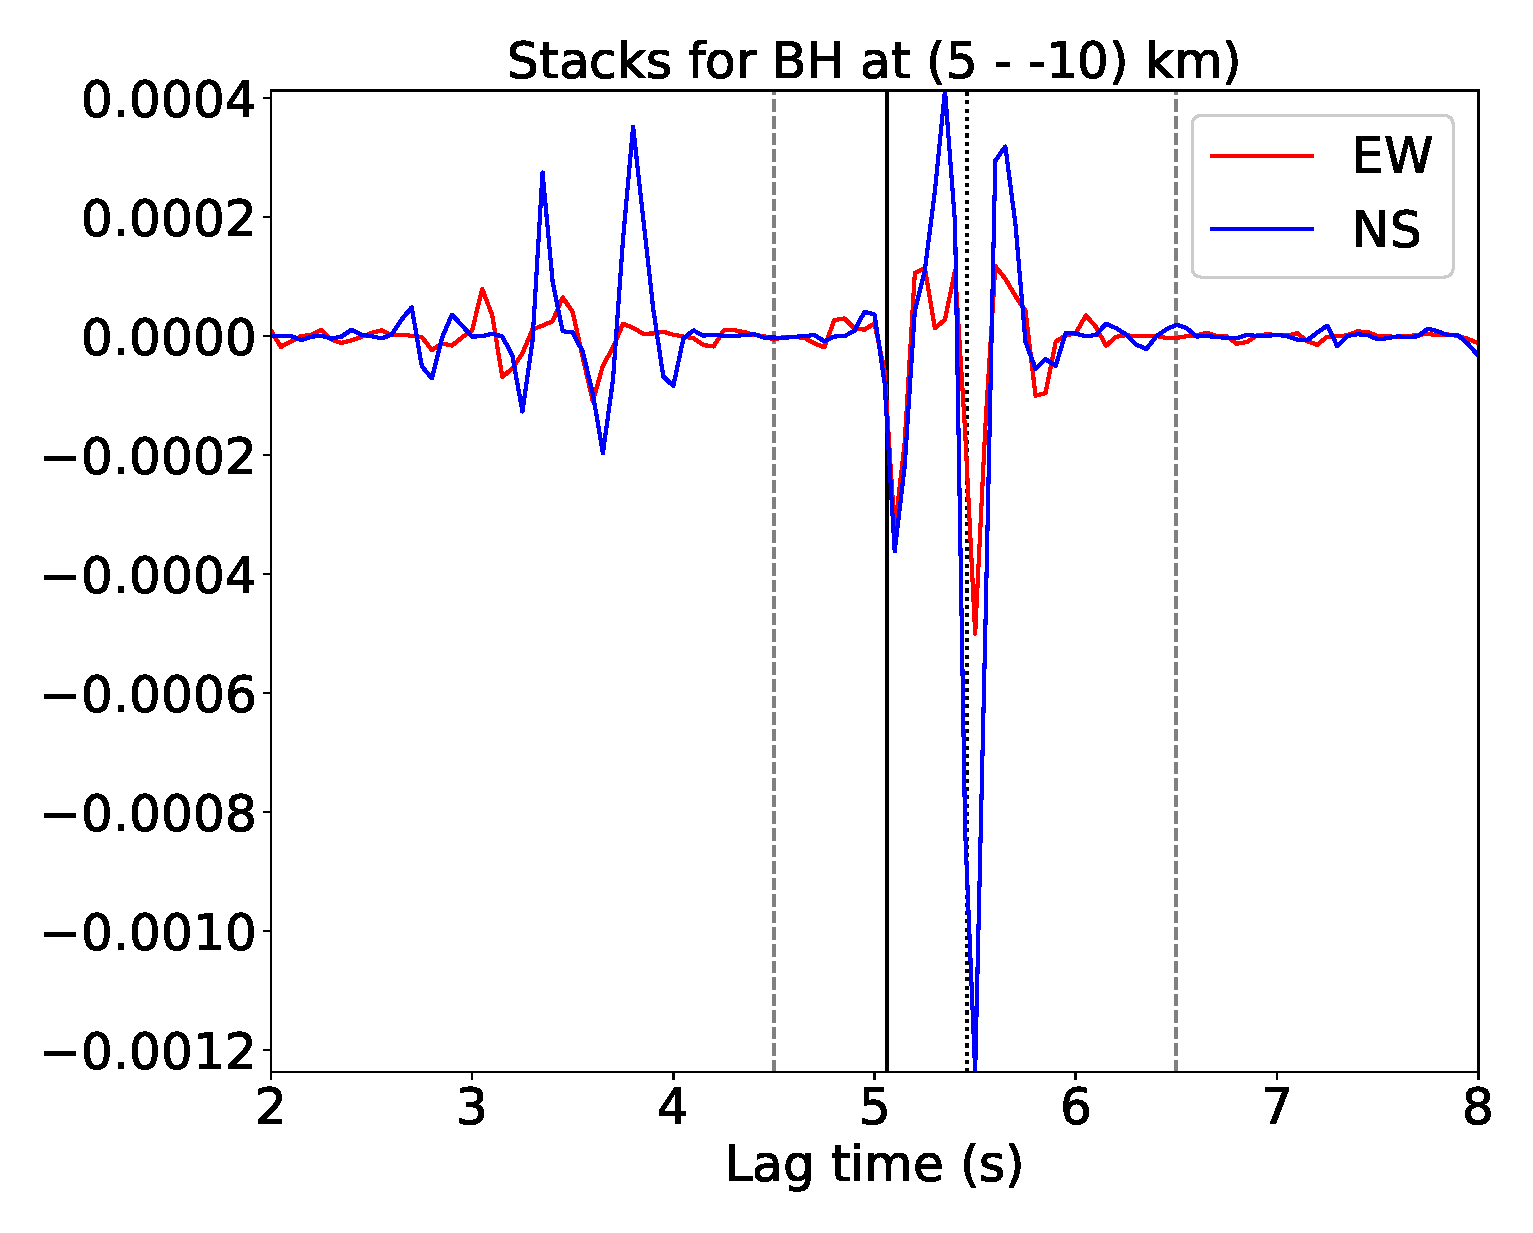
\includegraphics[width=\linewidth]{figures/intervals/BH_005_-10_stacks.eps}
\caption{See caption of Figure 1 for an explanation of this figure.}
\end{figure}

\begin{figure}[H]
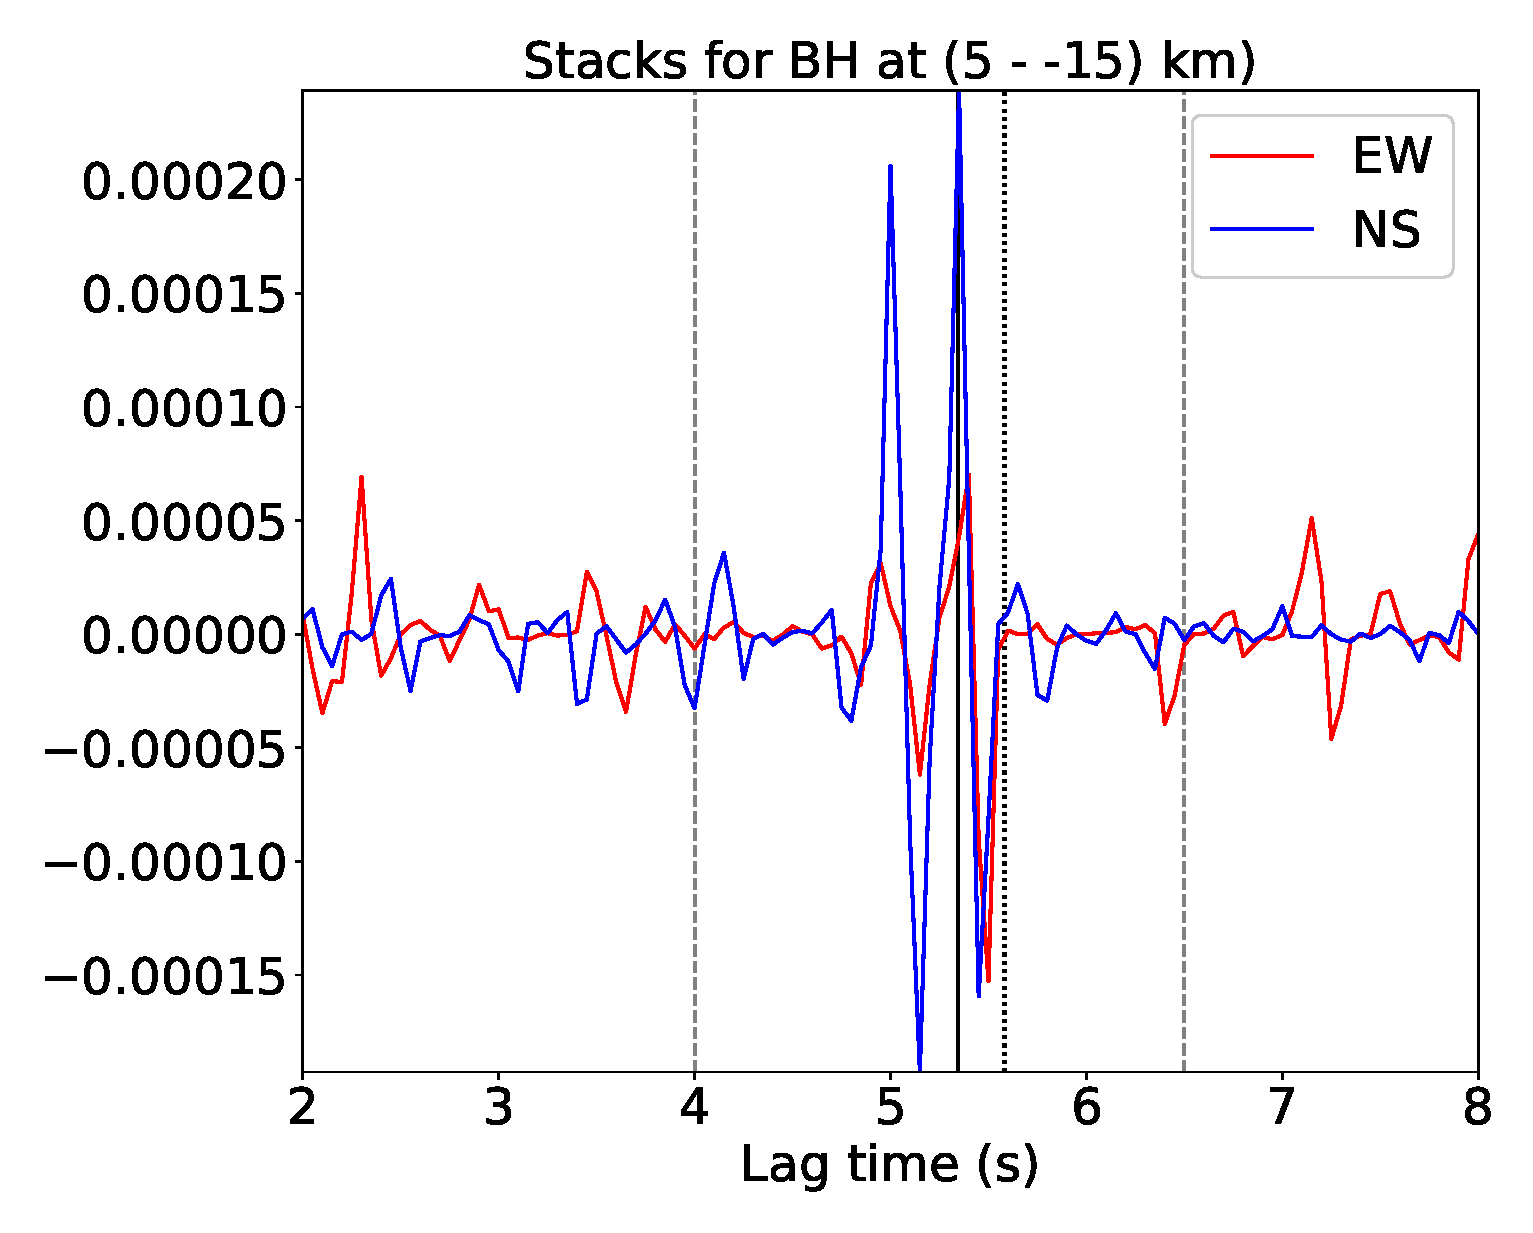
\includegraphics[width=\linewidth]{figures/intervals/BH_005_-15_stacks.eps}
\caption{See caption of Figure 1 for an explanation of this figure.}
\end{figure}

\begin{figure}[H]
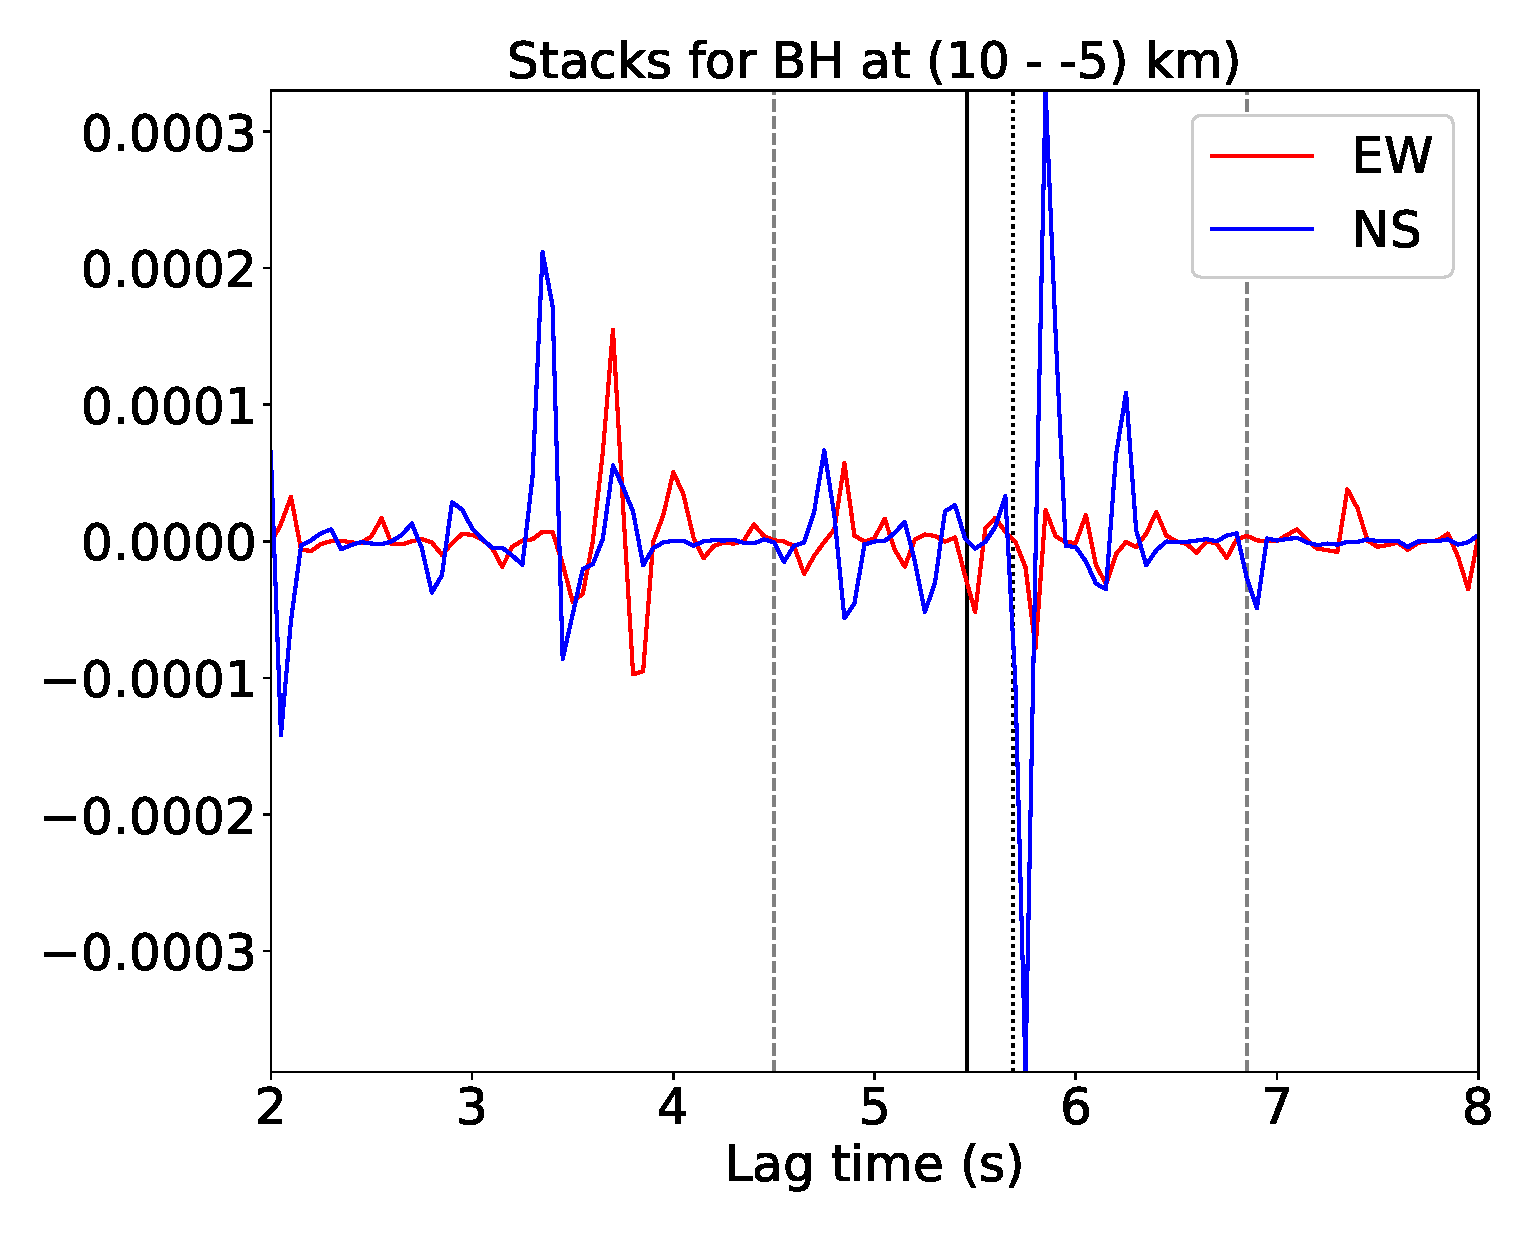
\includegraphics[width=\linewidth]{figures/intervals/BH_010_-05_stacks.eps}
\caption{See caption of Figure 1 for an explanation of this figure.}
\end{figure}

\begin{figure}[H]
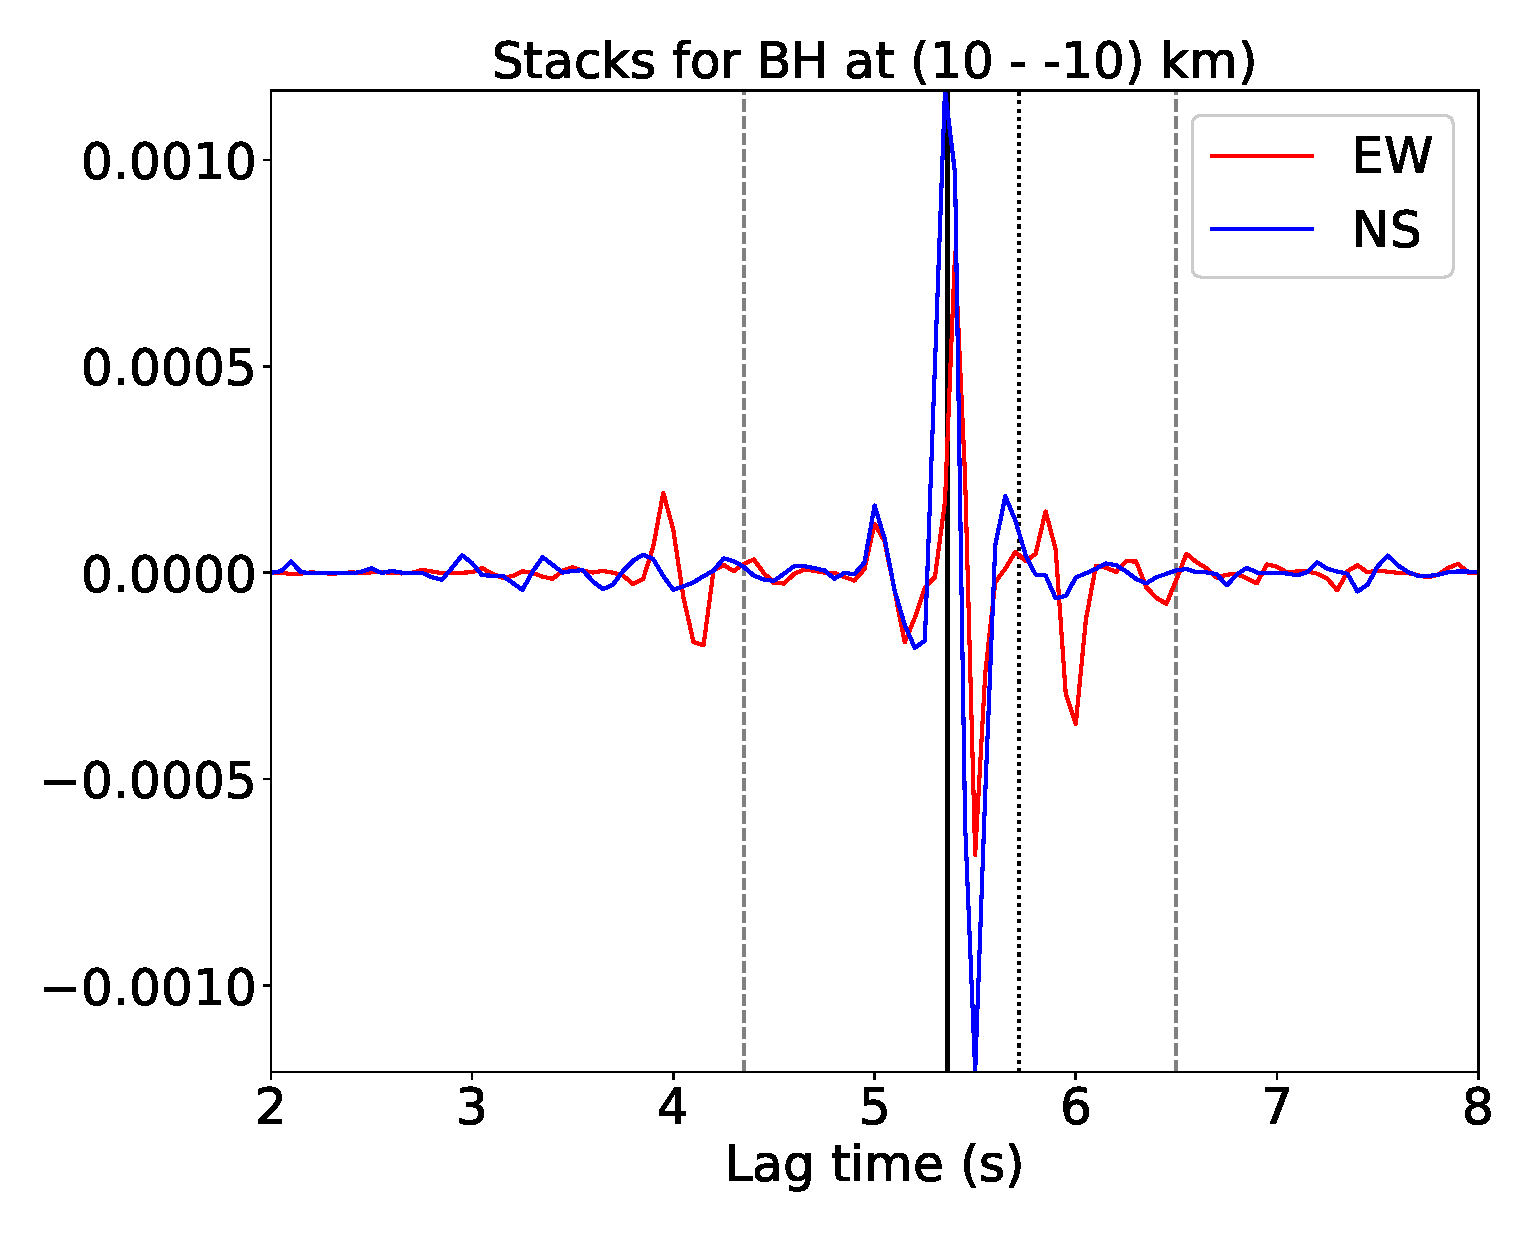
\includegraphics[width=\linewidth]{figures/intervals/BH_010_-10_stacks.eps}
\caption{See caption of Figure 1 for an explanation of this figure.}
\end{figure}

\begin{figure}[H]
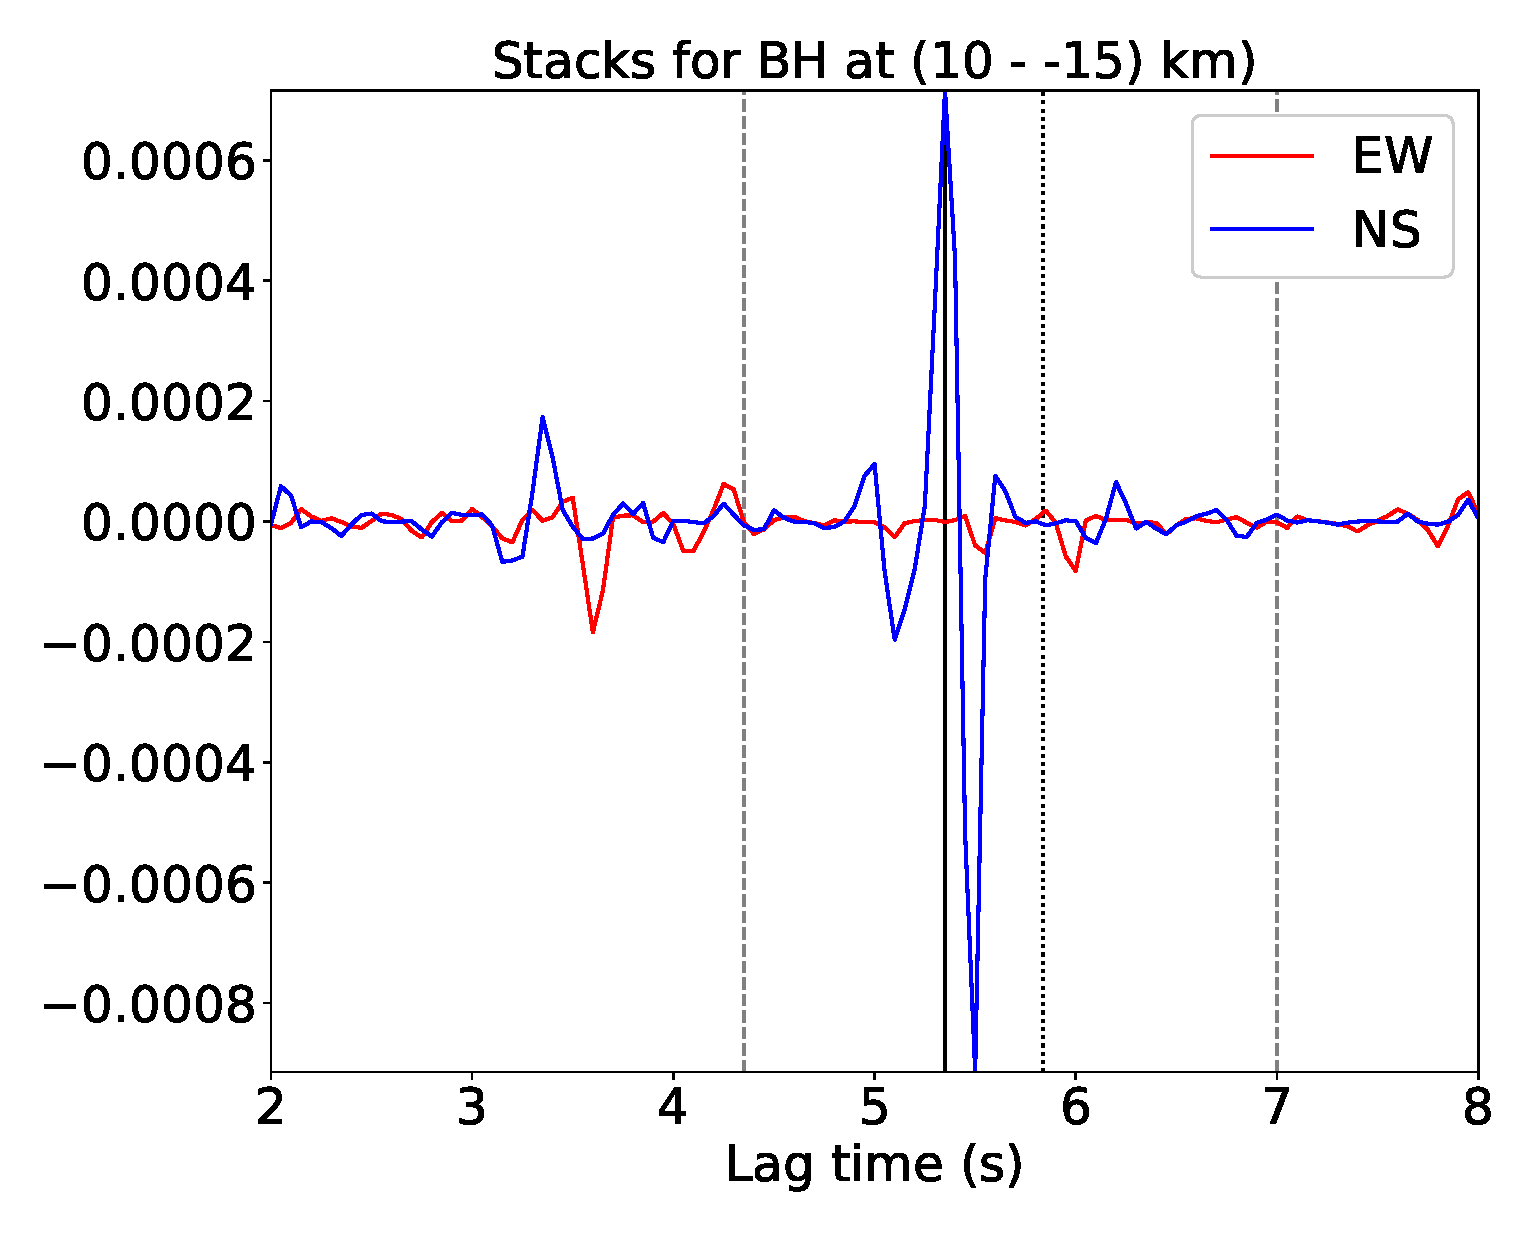
\includegraphics[width=\linewidth]{figures/intervals/BH_010_-15_stacks.eps}
\caption{See caption of Figure 1 for an explanation of this figure.}
\end{figure}

\begin{figure}[H]
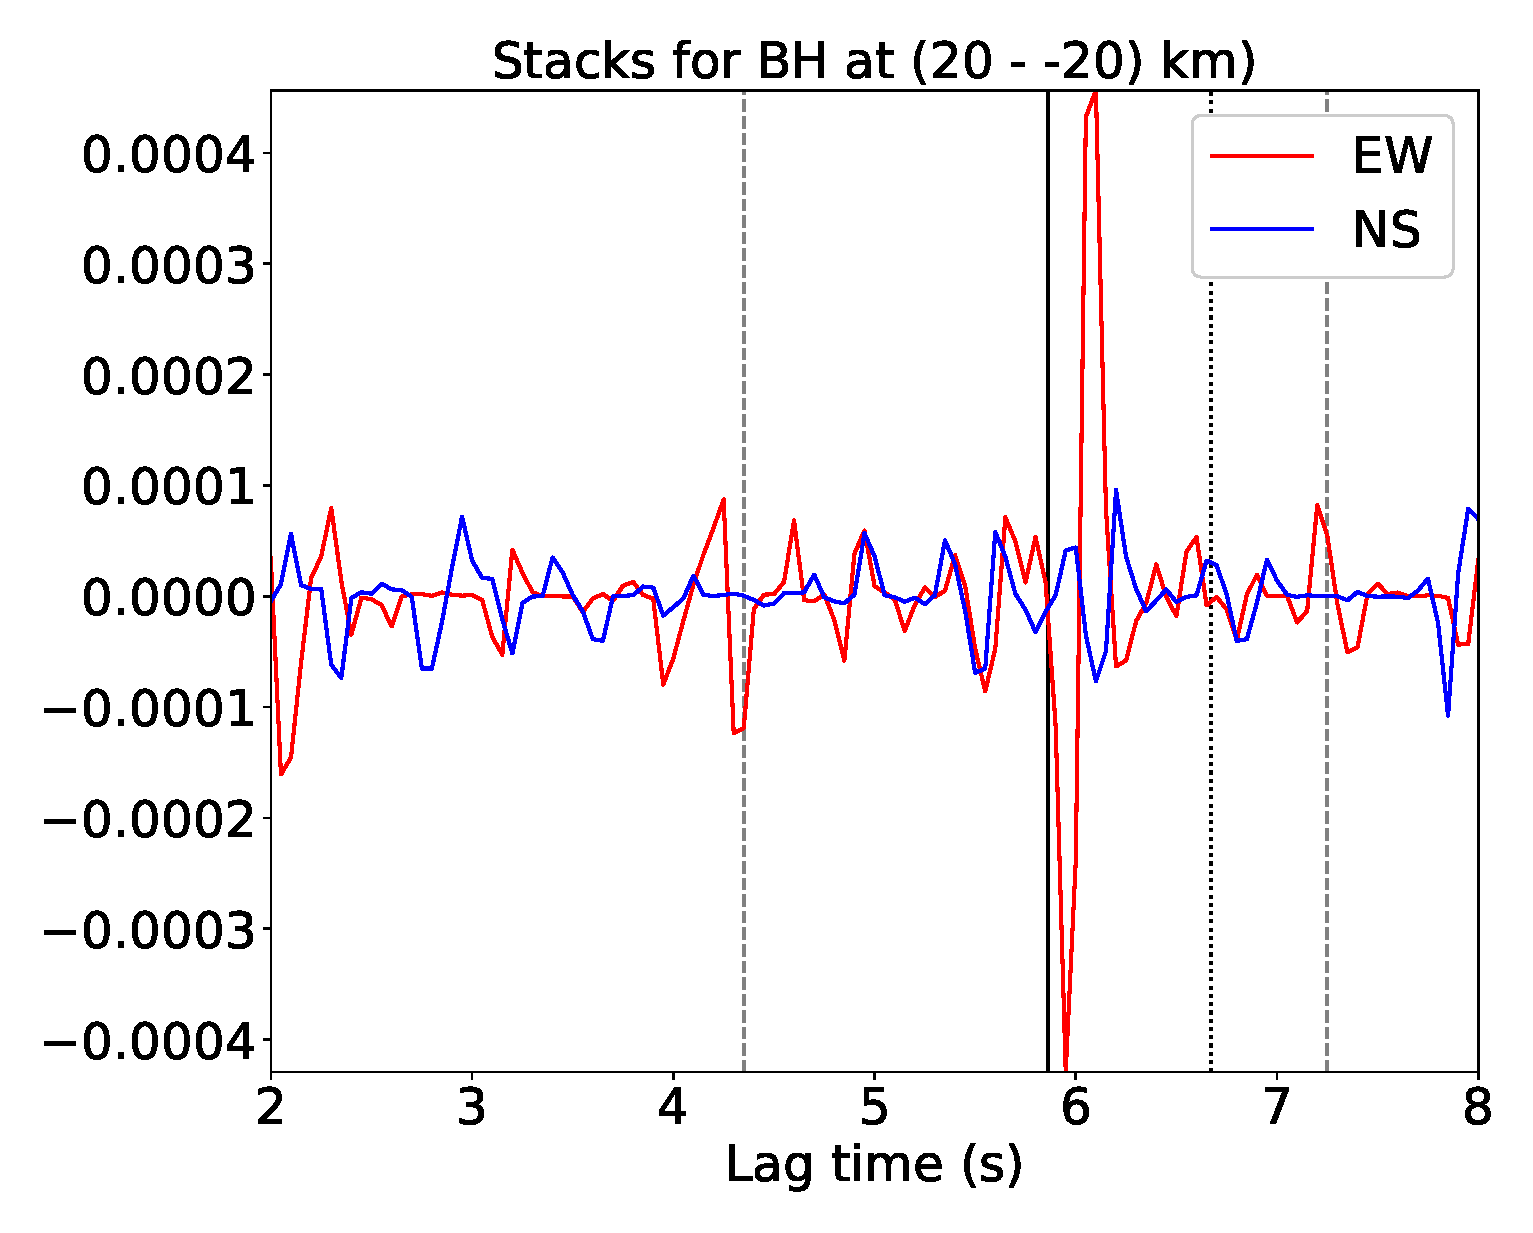
\includegraphics[width=\linewidth]{figures/intervals/BH_020_-20_stacks.eps}
\caption{See caption of Figure 1 for an explanation of this figure.}
\end{figure}

\begin{figure}[H]
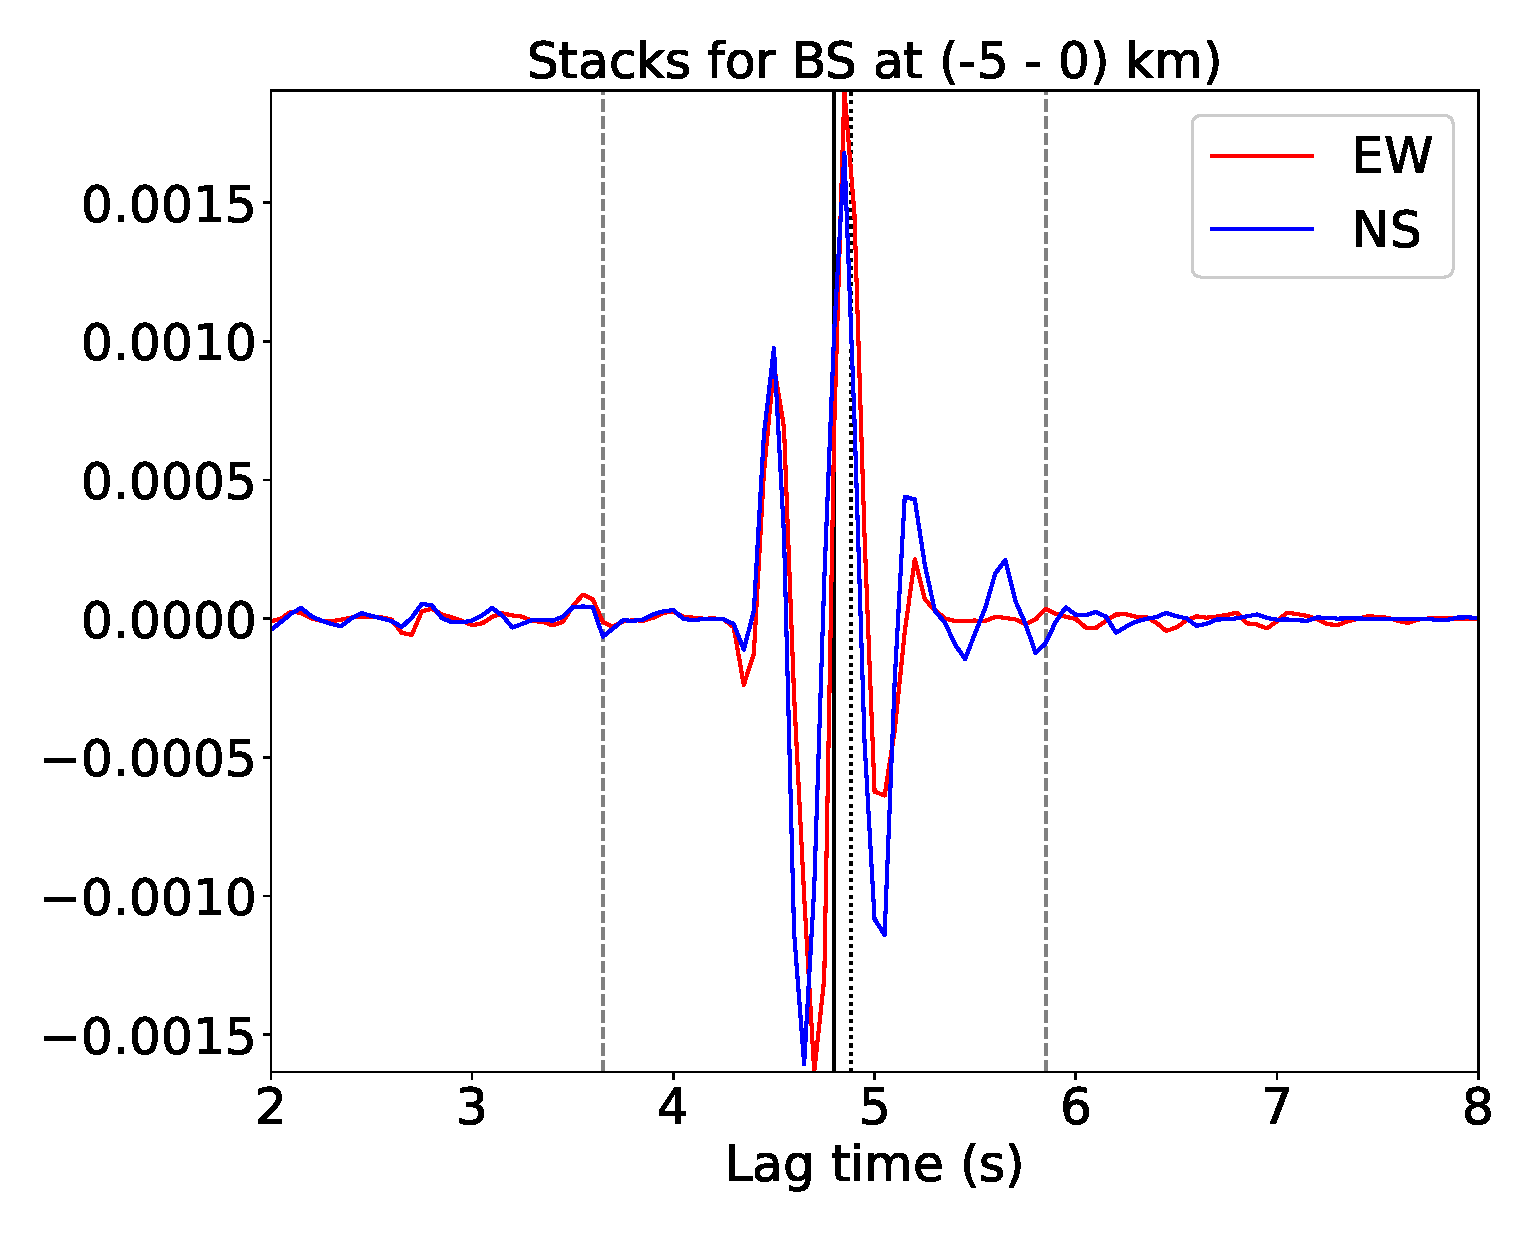
\includegraphics[width=\linewidth]{figures/intervals/BS_-05_000_stacks.eps}
\caption{See caption of Figure 1 for an explanation of this figure.}
\end{figure}

\begin{figure}[H]
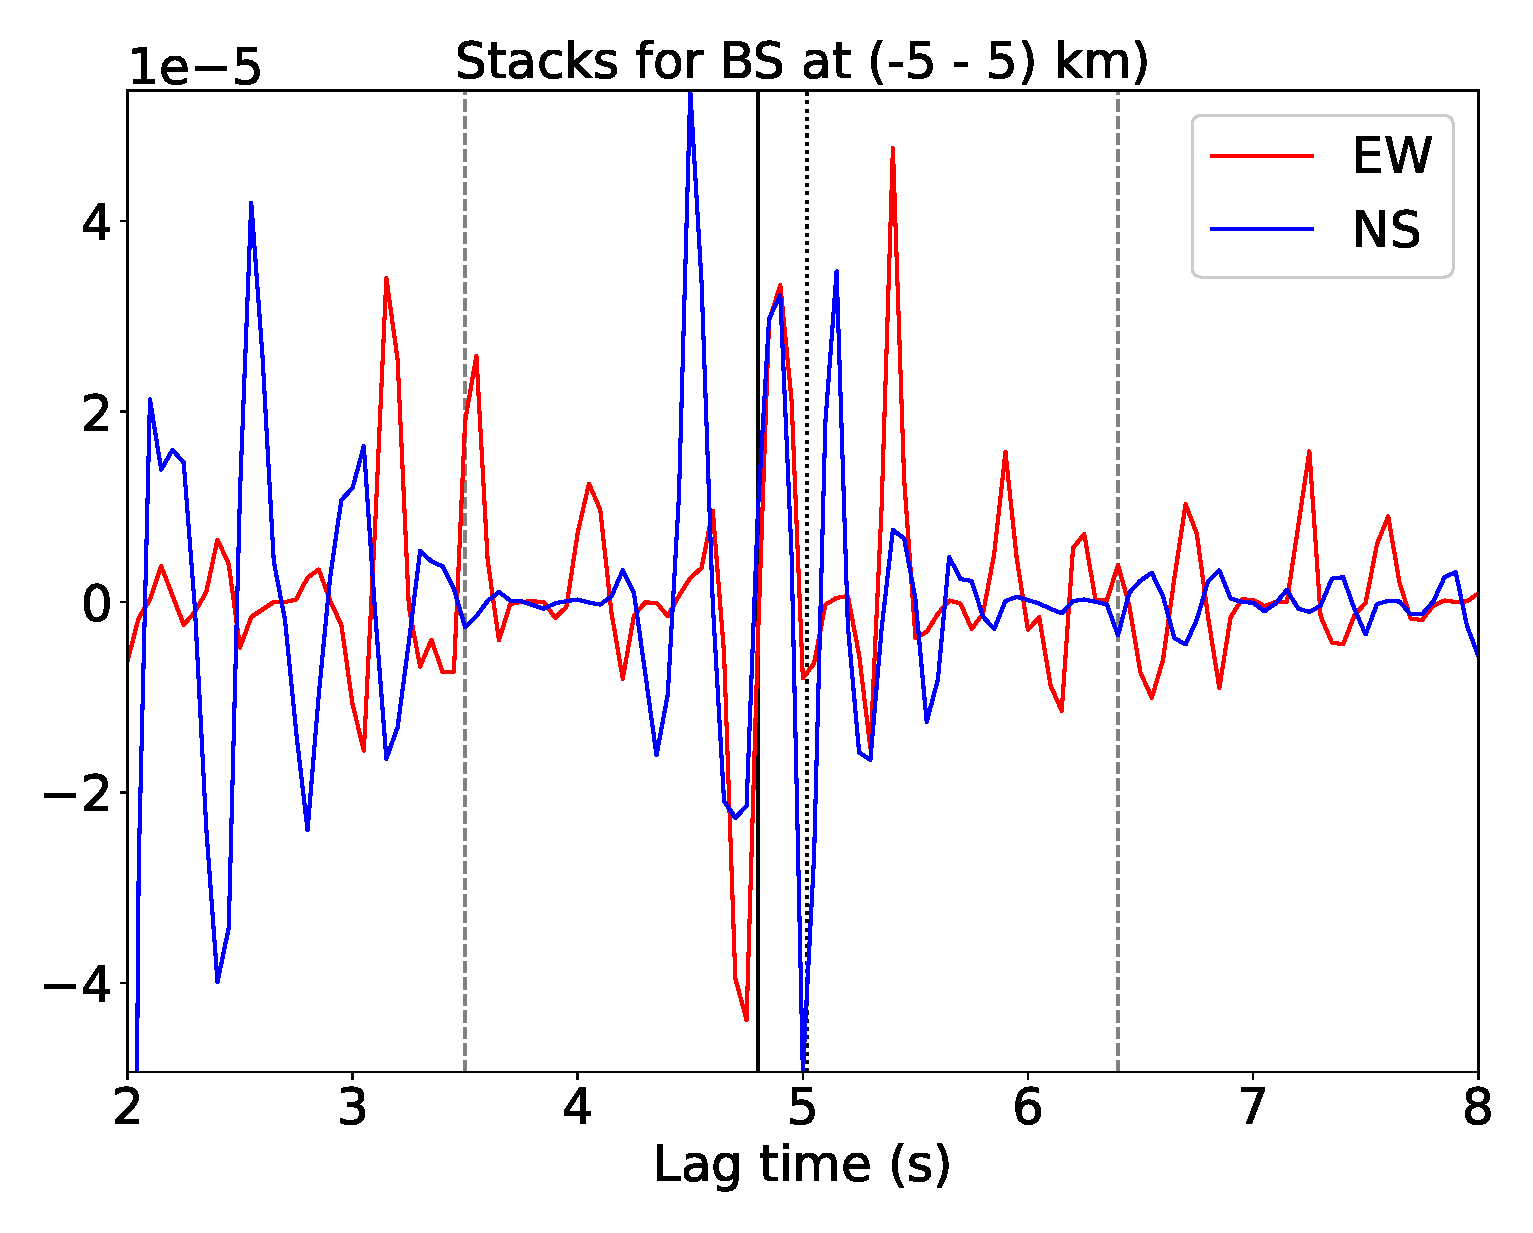
\includegraphics[width=\linewidth]{figures/intervals/BS_-05_005_stacks.eps}
\caption{See caption of Figure 1 for an explanation of this figure.}
\end{figure}

\begin{figure}[H]
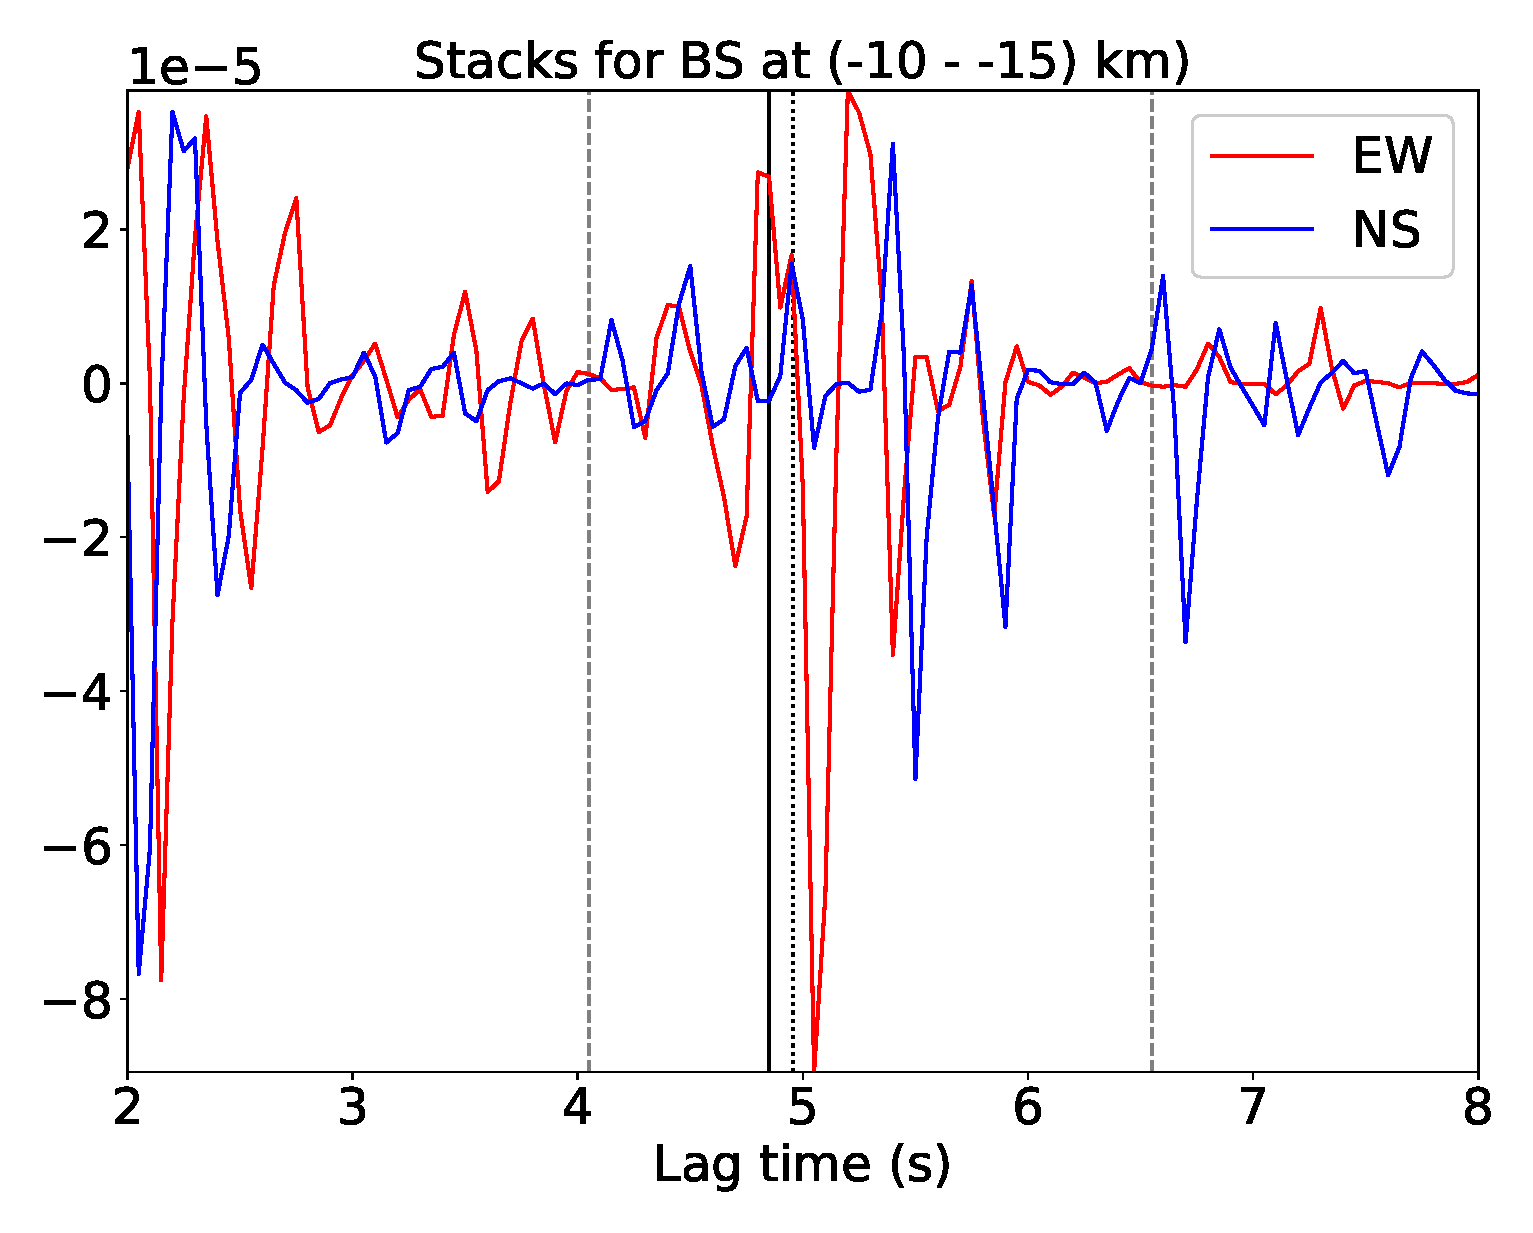
\includegraphics[width=\linewidth]{figures/intervals/BS_-10_-15_stacks.eps}
\caption{See caption of Figure 1 for an explanation of this figure.}
\end{figure}

\begin{figure}[H]
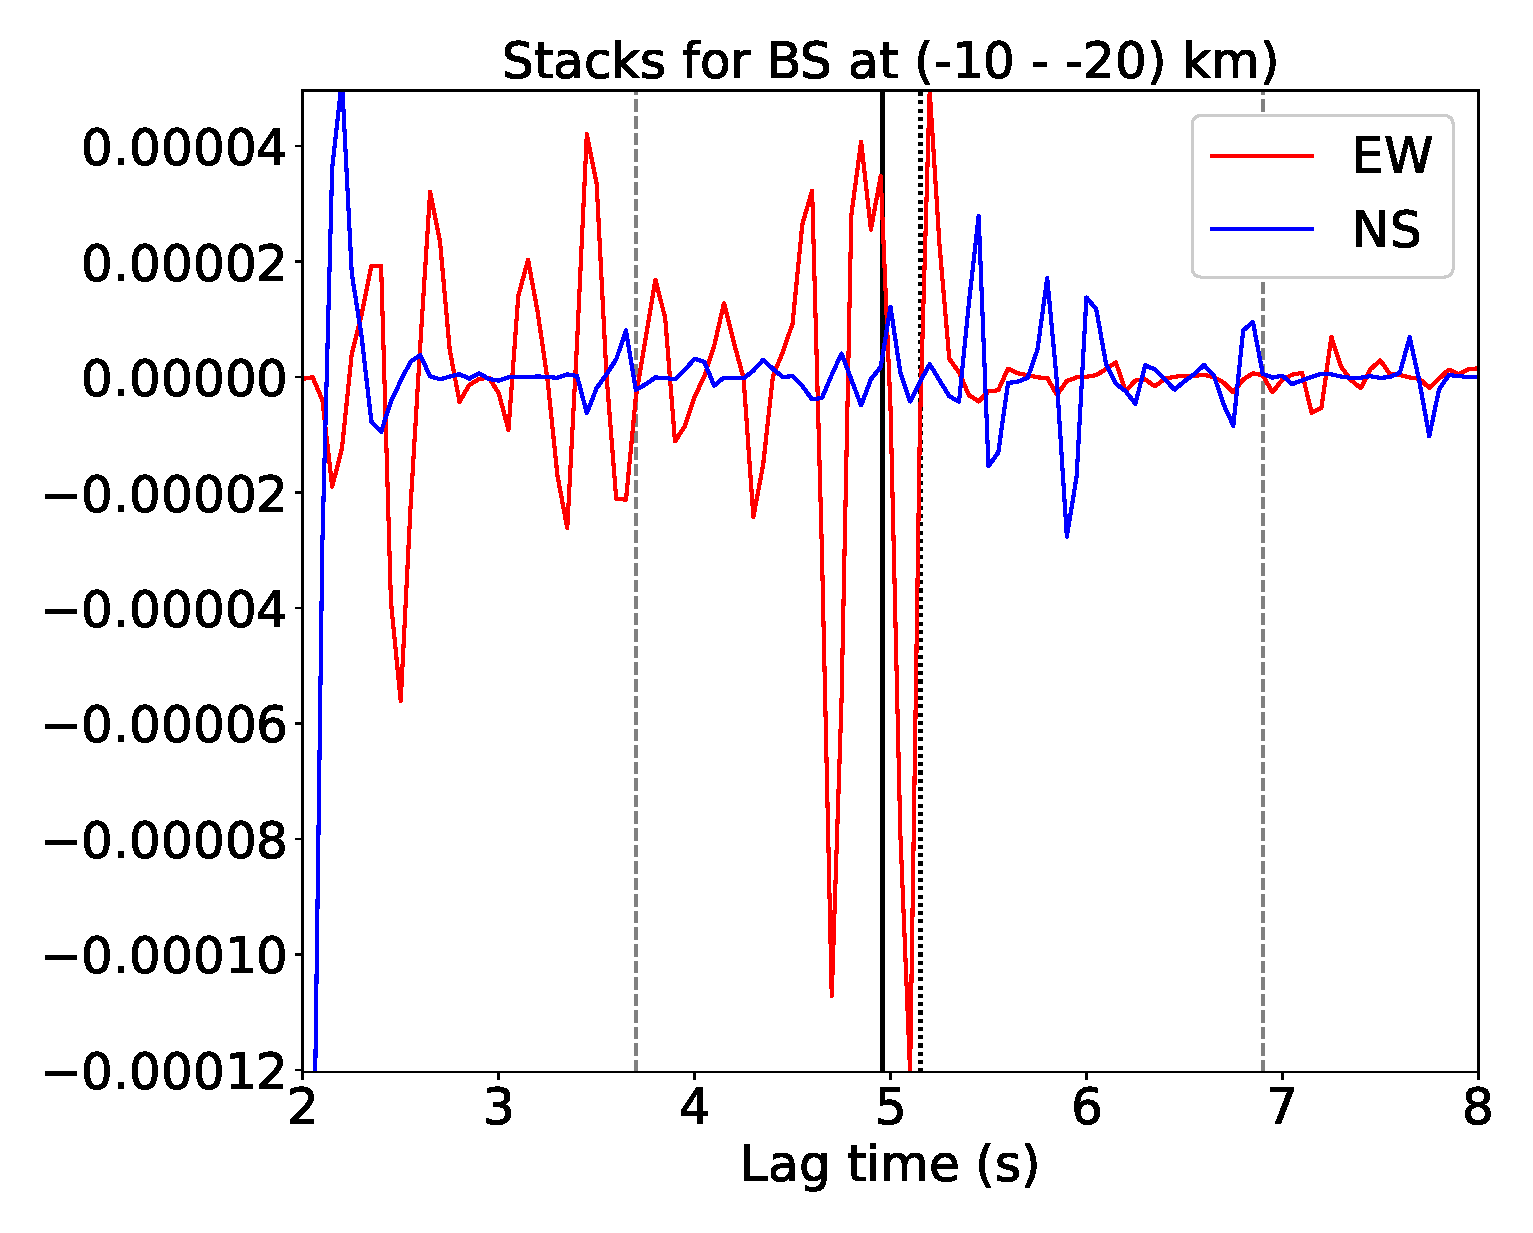
\includegraphics[width=\linewidth]{figures/intervals/BS_-10_-20_stacks.eps}
\caption{See caption of Figure 1 for an explanation of this figure.}
\end{figure}

\begin{figure}[H]
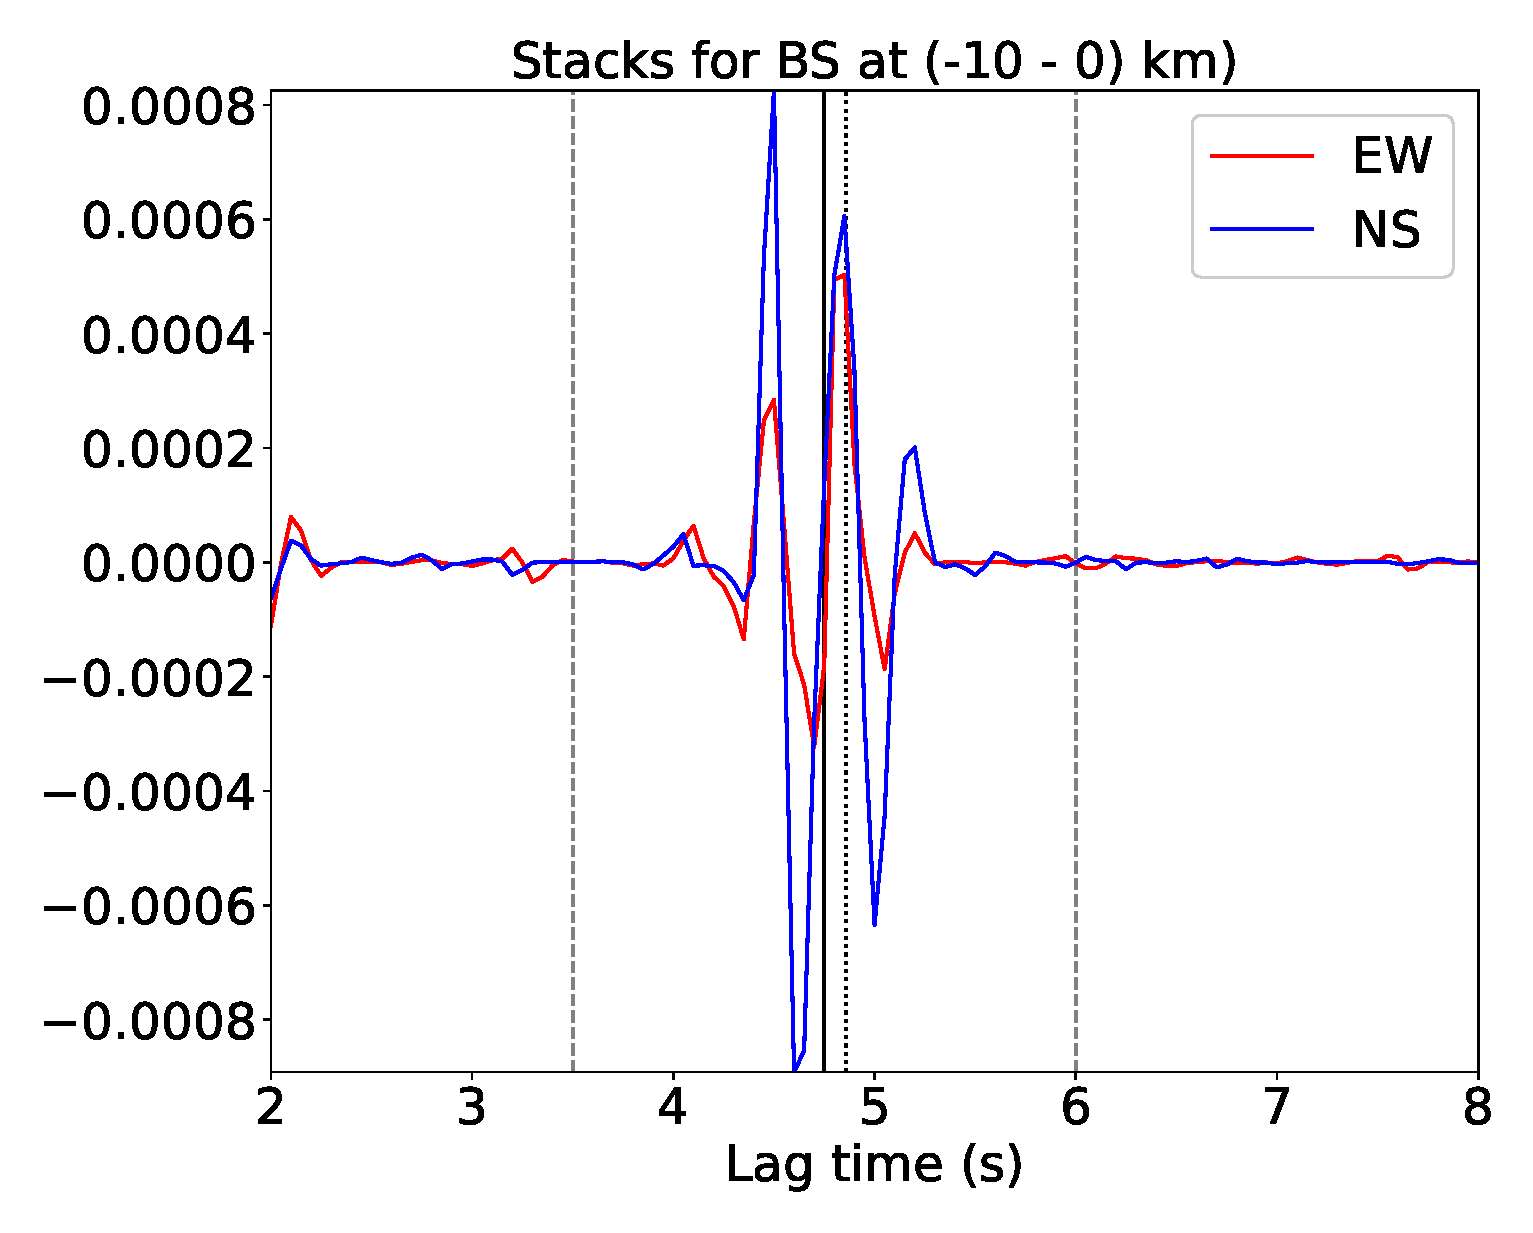
\includegraphics[width=\linewidth]{figures/intervals/BS_-10_000_stacks.eps}
\caption{See caption of Figure 1 for an explanation of this figure.}
\end{figure}

\begin{figure}[H]
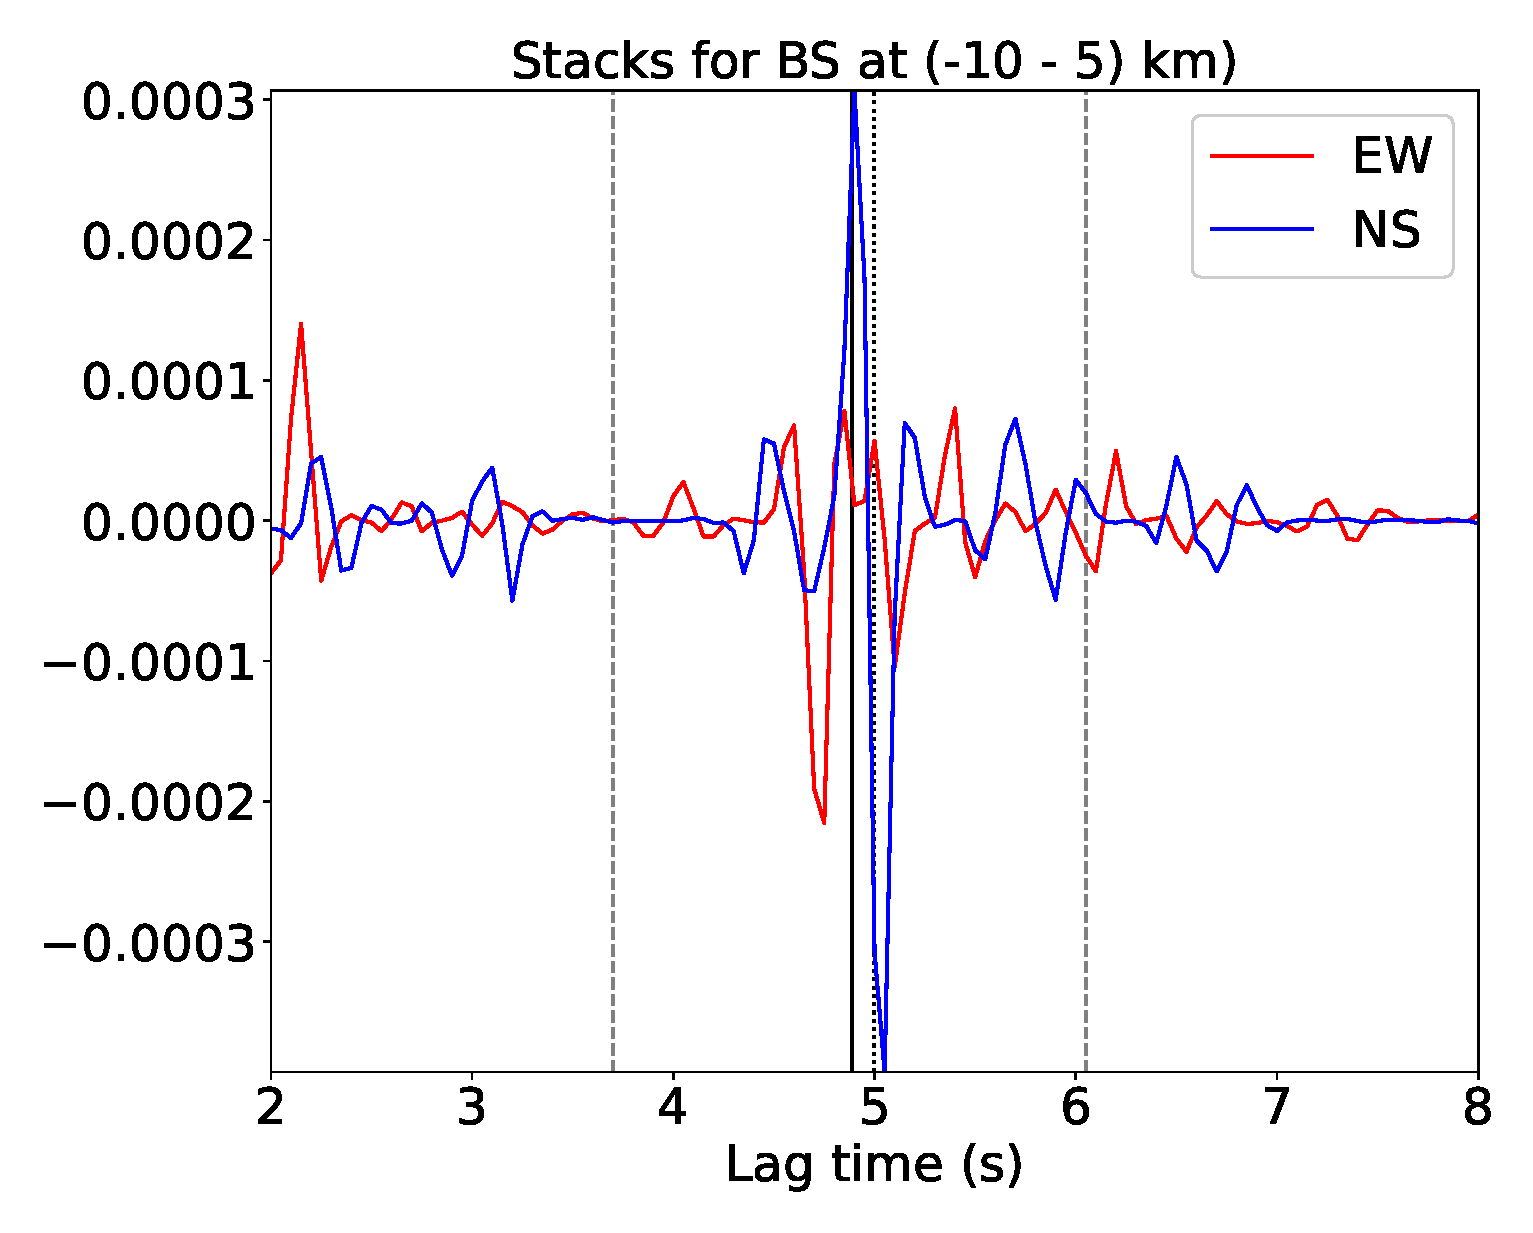
\includegraphics[width=\linewidth]{figures/intervals/BS_-10_005_stacks.eps}
\caption{See caption of Figure 1 for an explanation of this figure.}
\end{figure}

\begin{figure}[H]
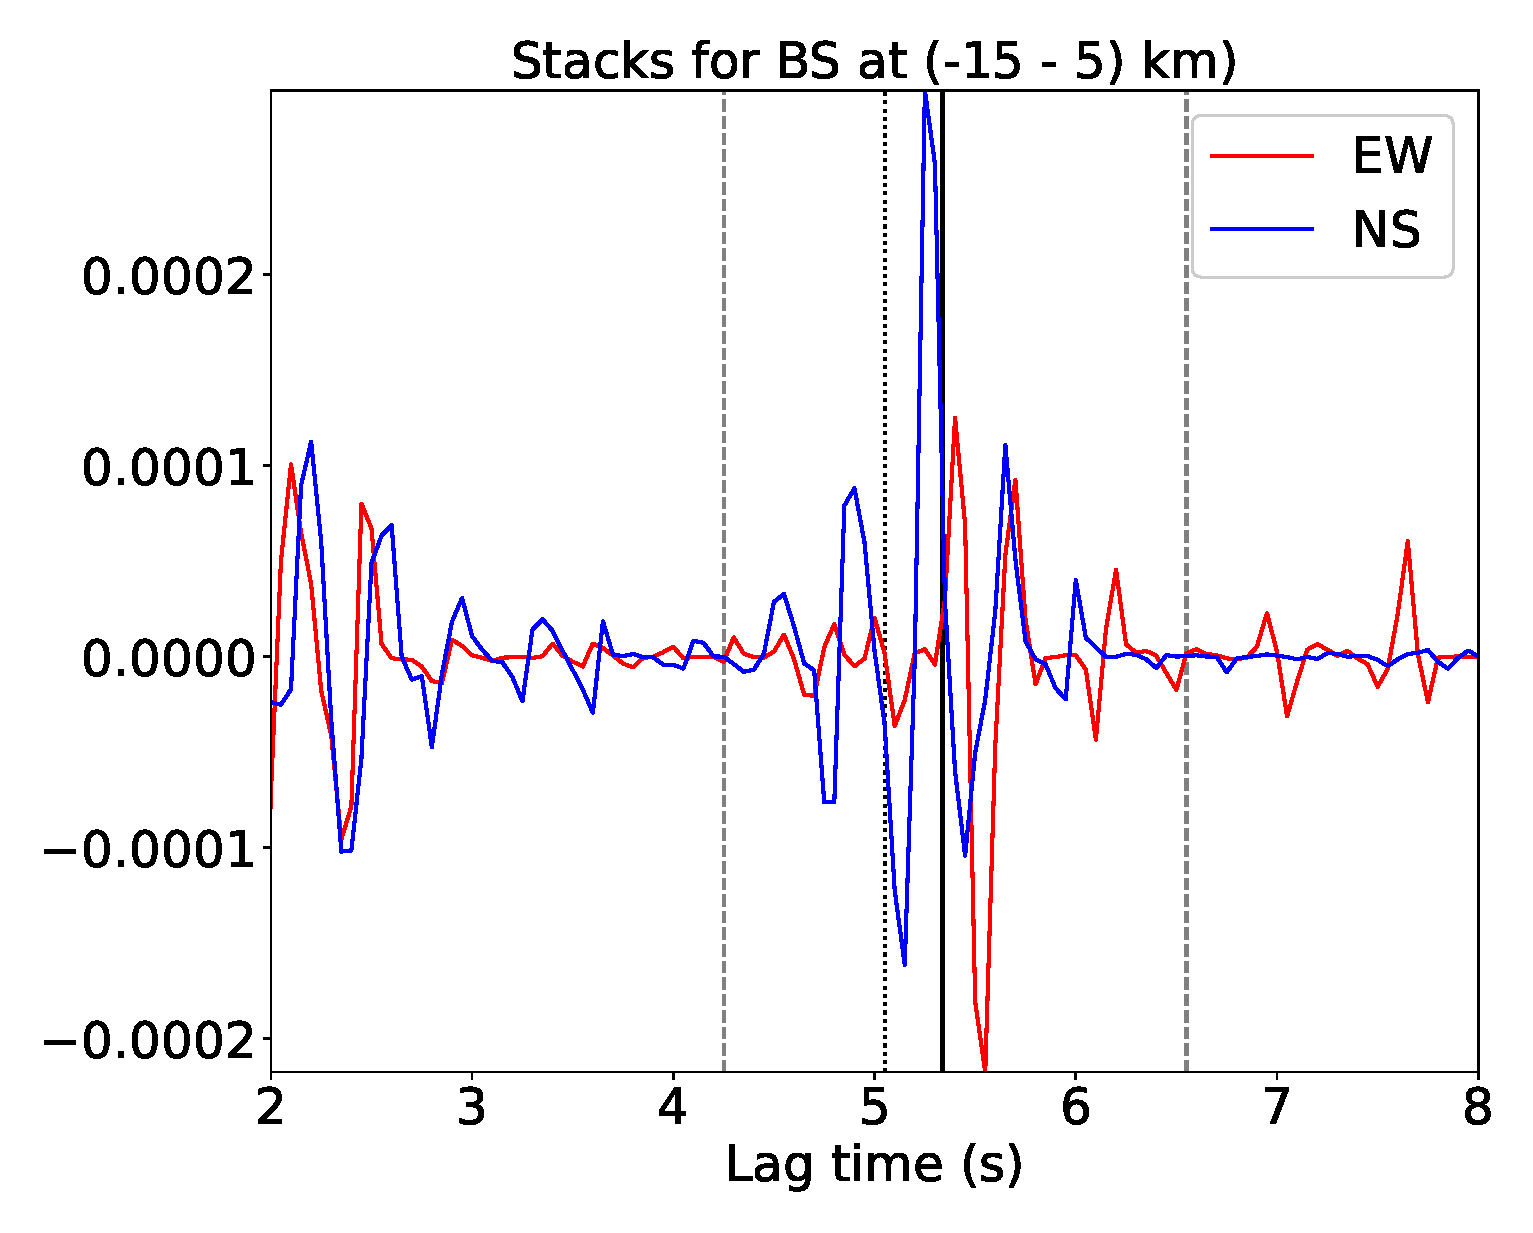
\includegraphics[width=\linewidth]{figures/intervals/BS_-15_005_stacks.eps}
\caption{See caption of Figure 1 for an explanation of this figure.}
\end{figure}

\begin{figure}[H]
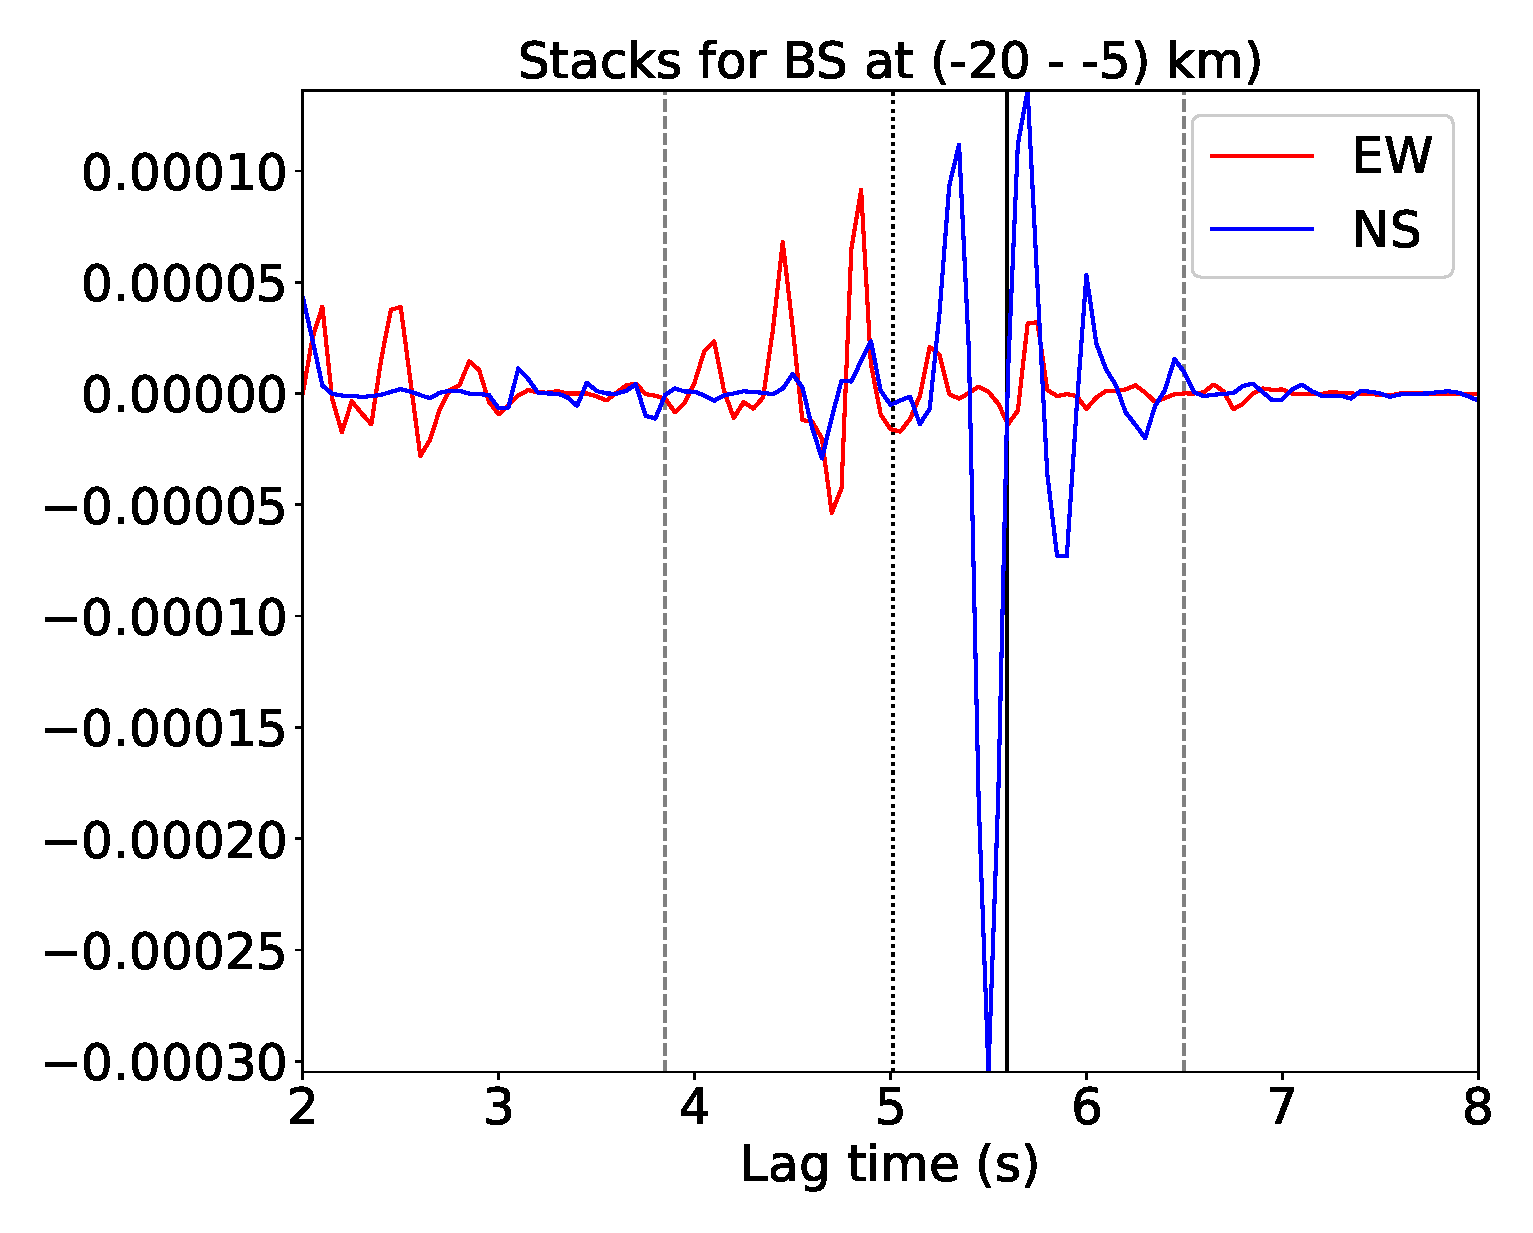
\includegraphics[width=\linewidth]{figures/intervals/BS_-20_-05_stacks.eps}
\caption{See caption of Figure 1 for an explanation of this figure.}
\end{figure}

\begin{figure}[H]
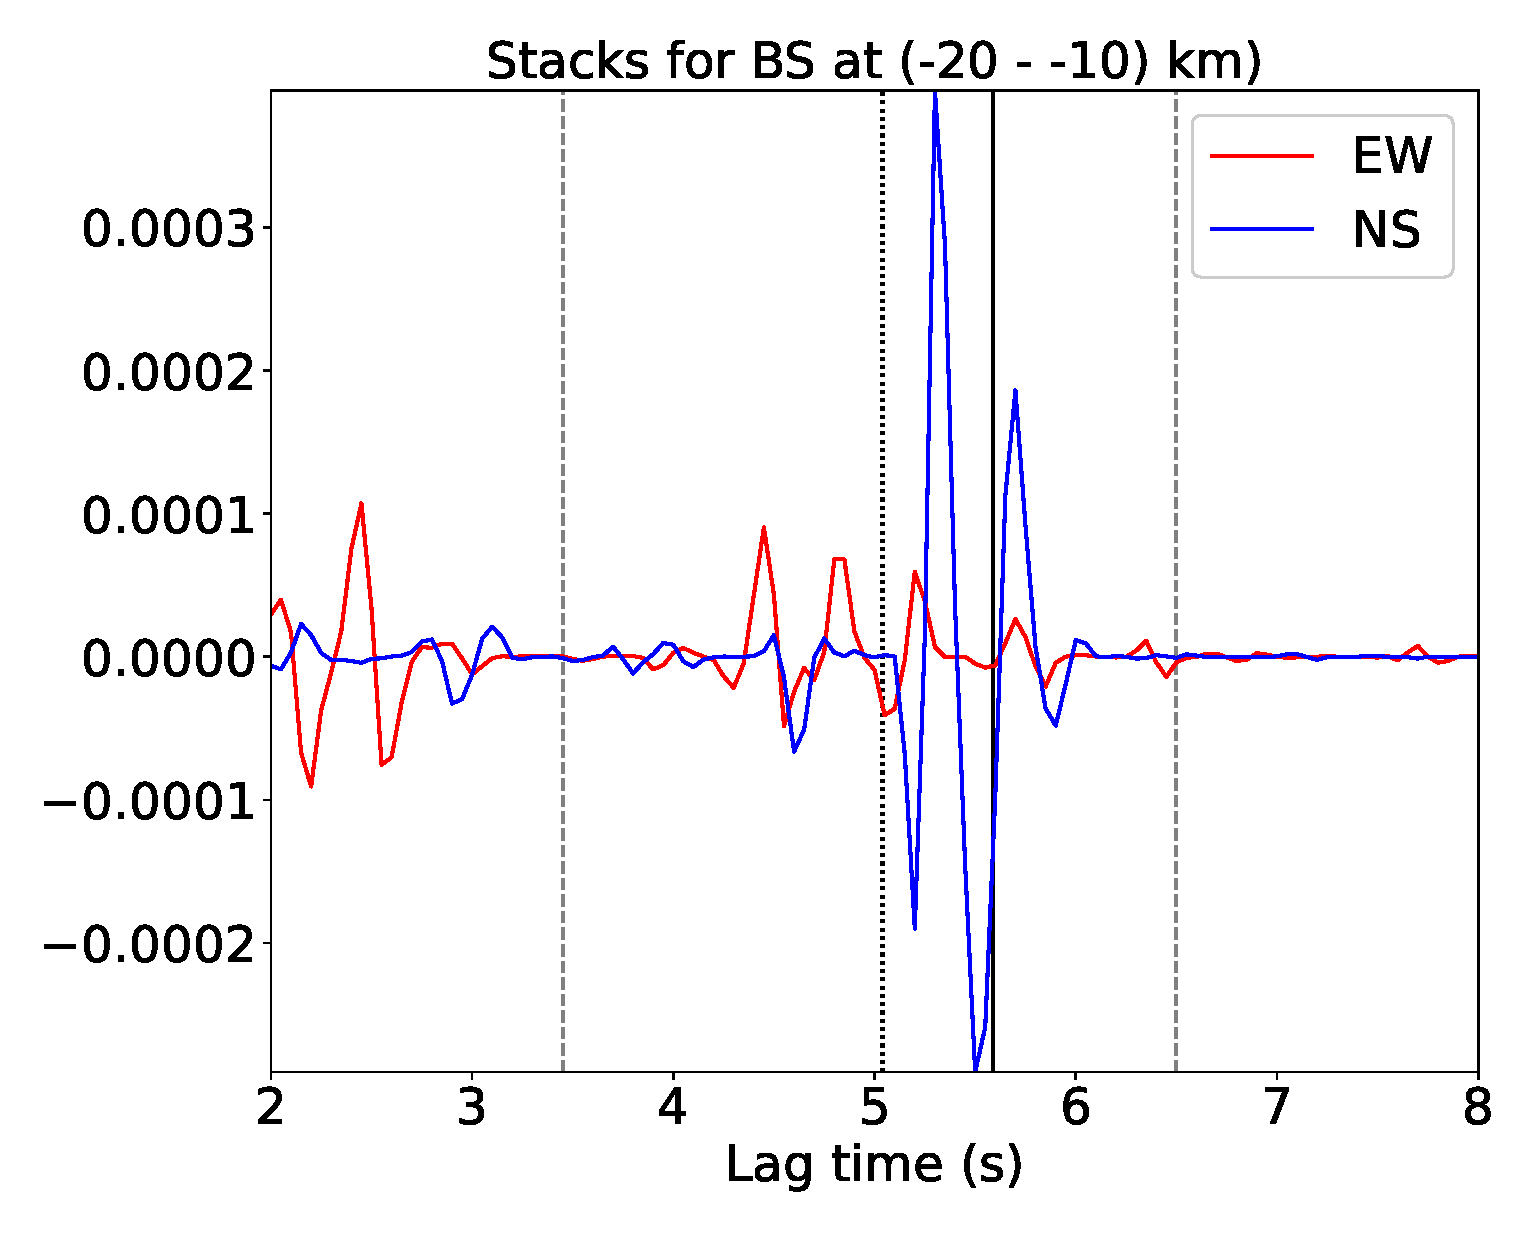
\includegraphics[width=\linewidth]{figures/intervals/BS_-20_-10_stacks.eps}
\caption{See caption of Figure 1 for an explanation of this figure.}
\end{figure}

\begin{figure}[H]
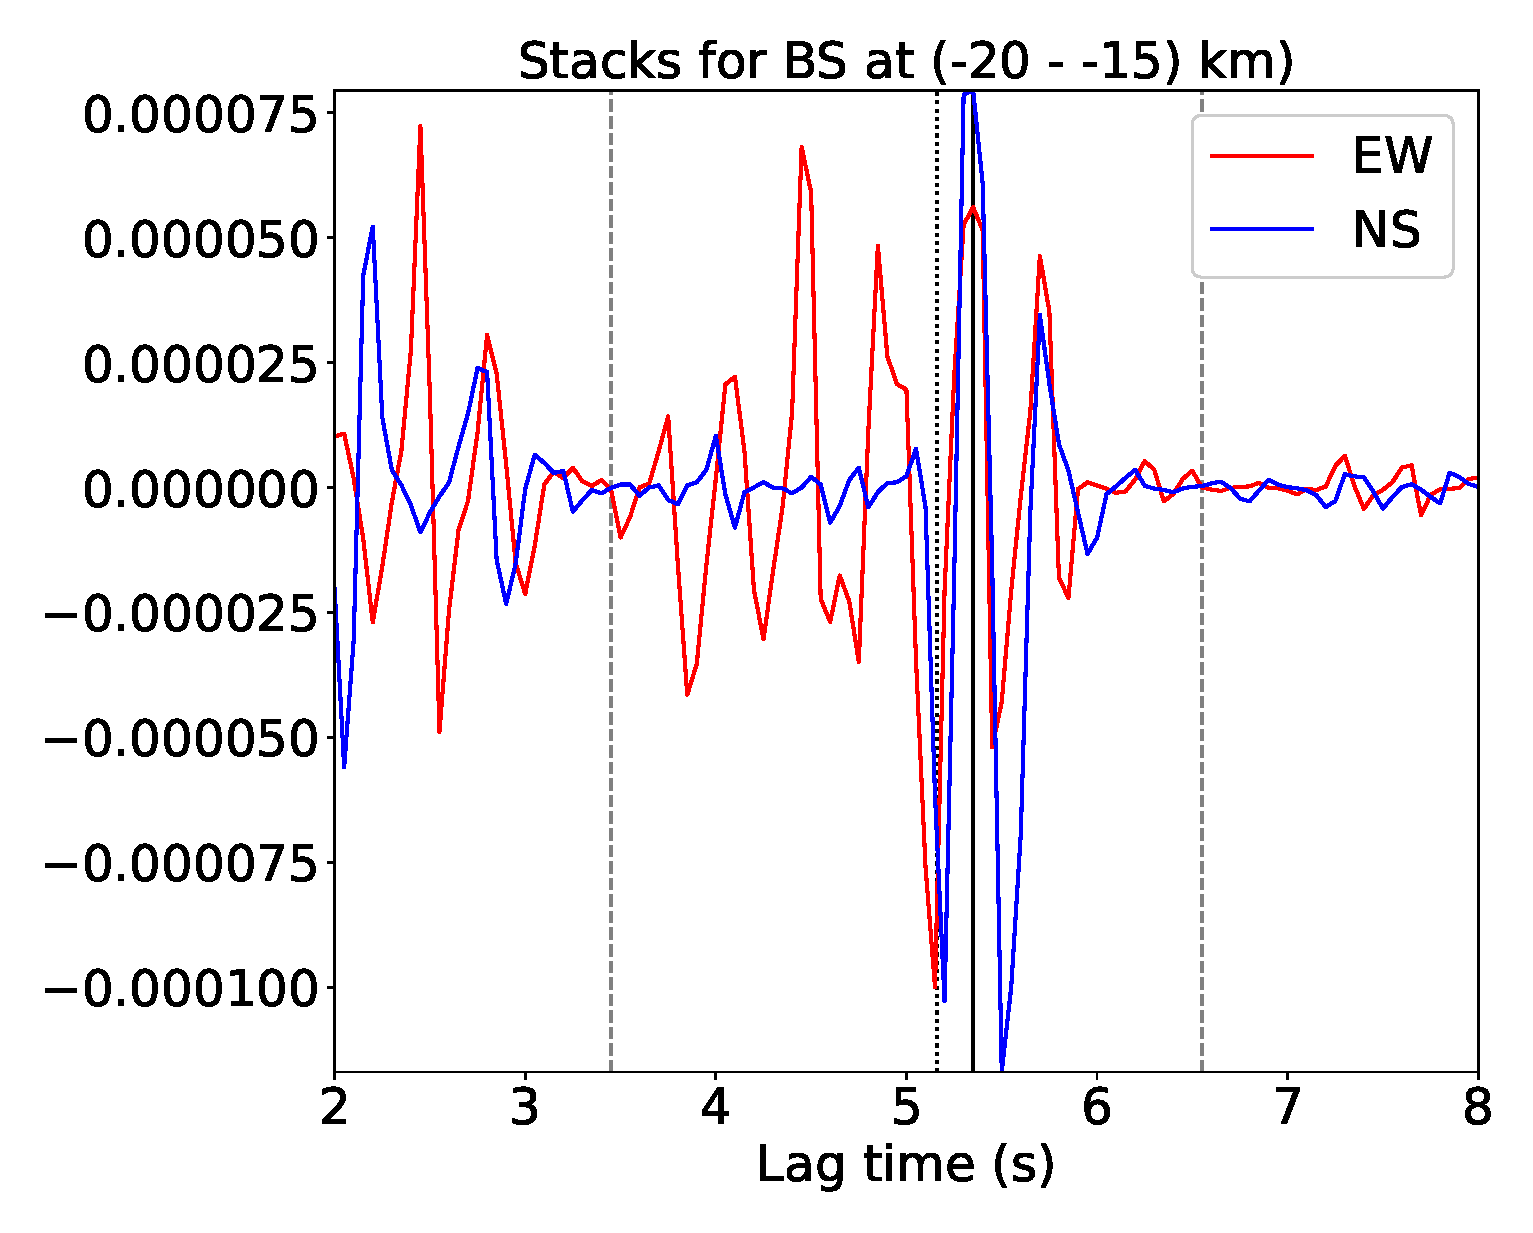
\includegraphics[width=\linewidth]{figures/intervals/BS_-20_-15_stacks.eps}
\caption{See caption of Figure 1 for an explanation of this figure.}
\end{figure}

\begin{figure}[H]
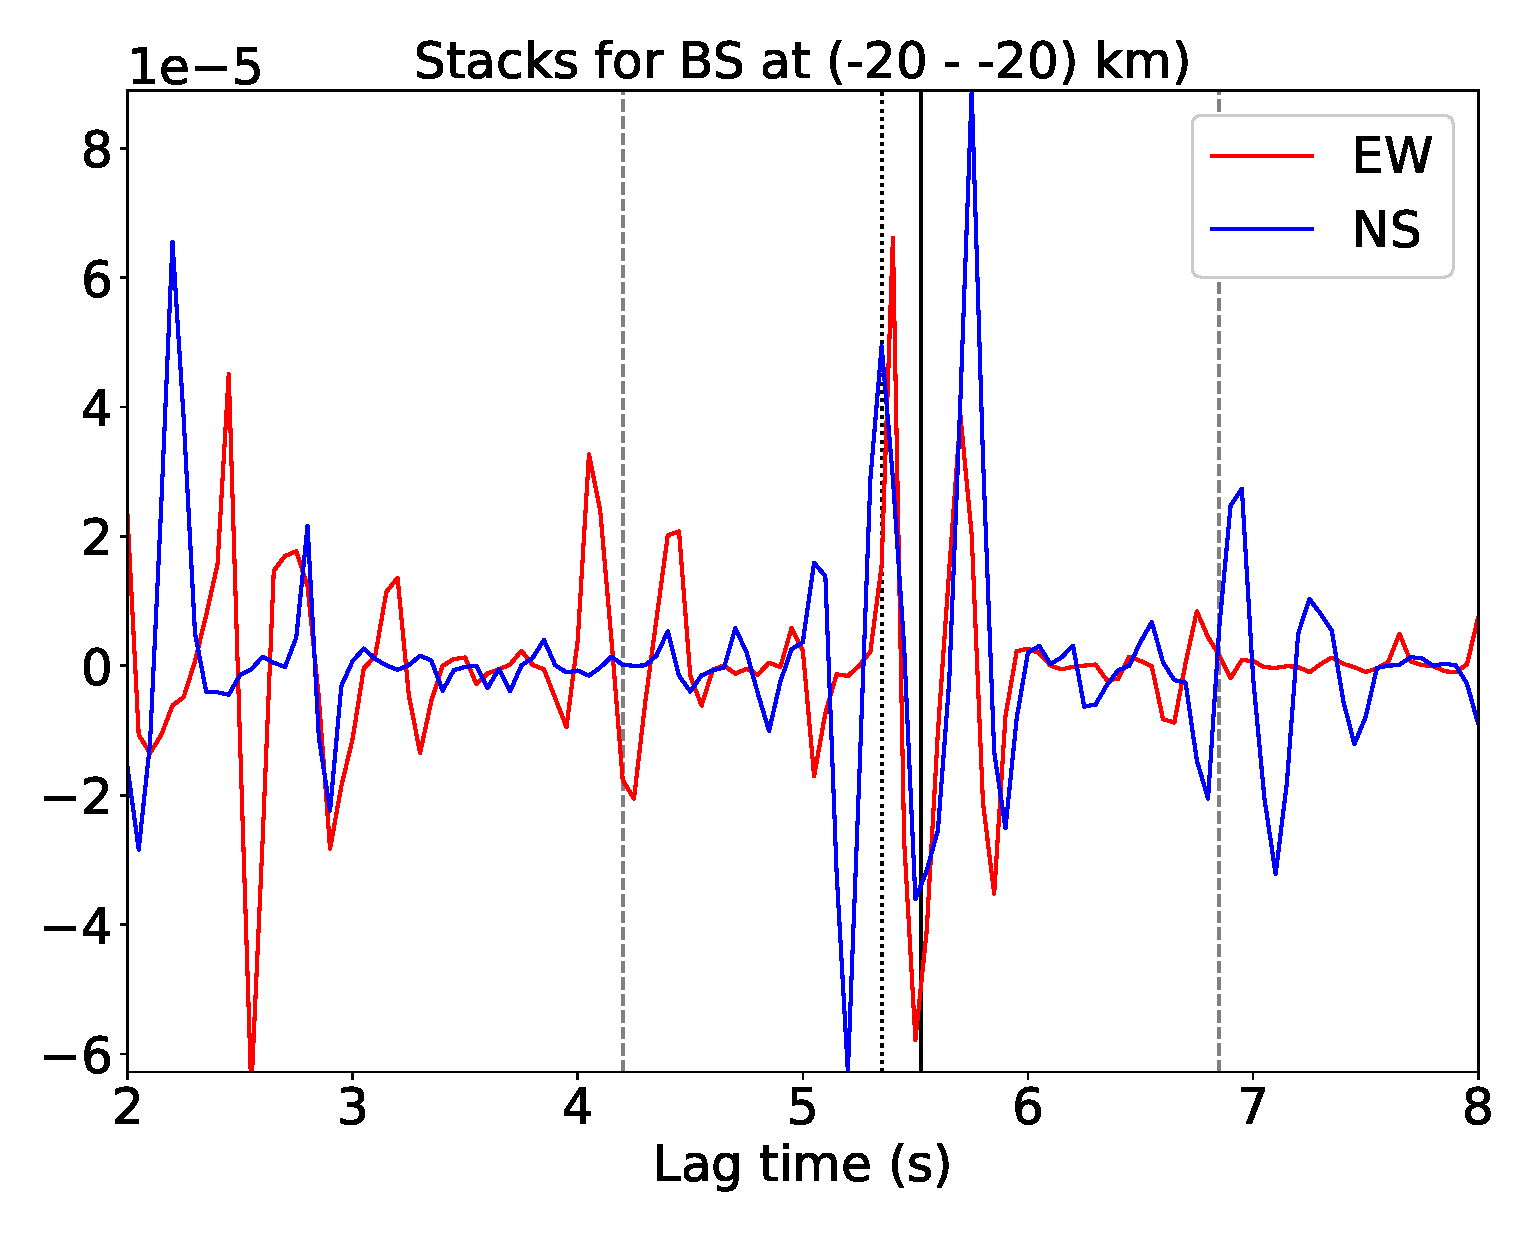
\includegraphics[width=\linewidth]{figures/intervals/BS_-20_-20_stacks.eps}
\caption{See caption of Figure 1 for an explanation of this figure.}
\end{figure}

\begin{figure}[H]
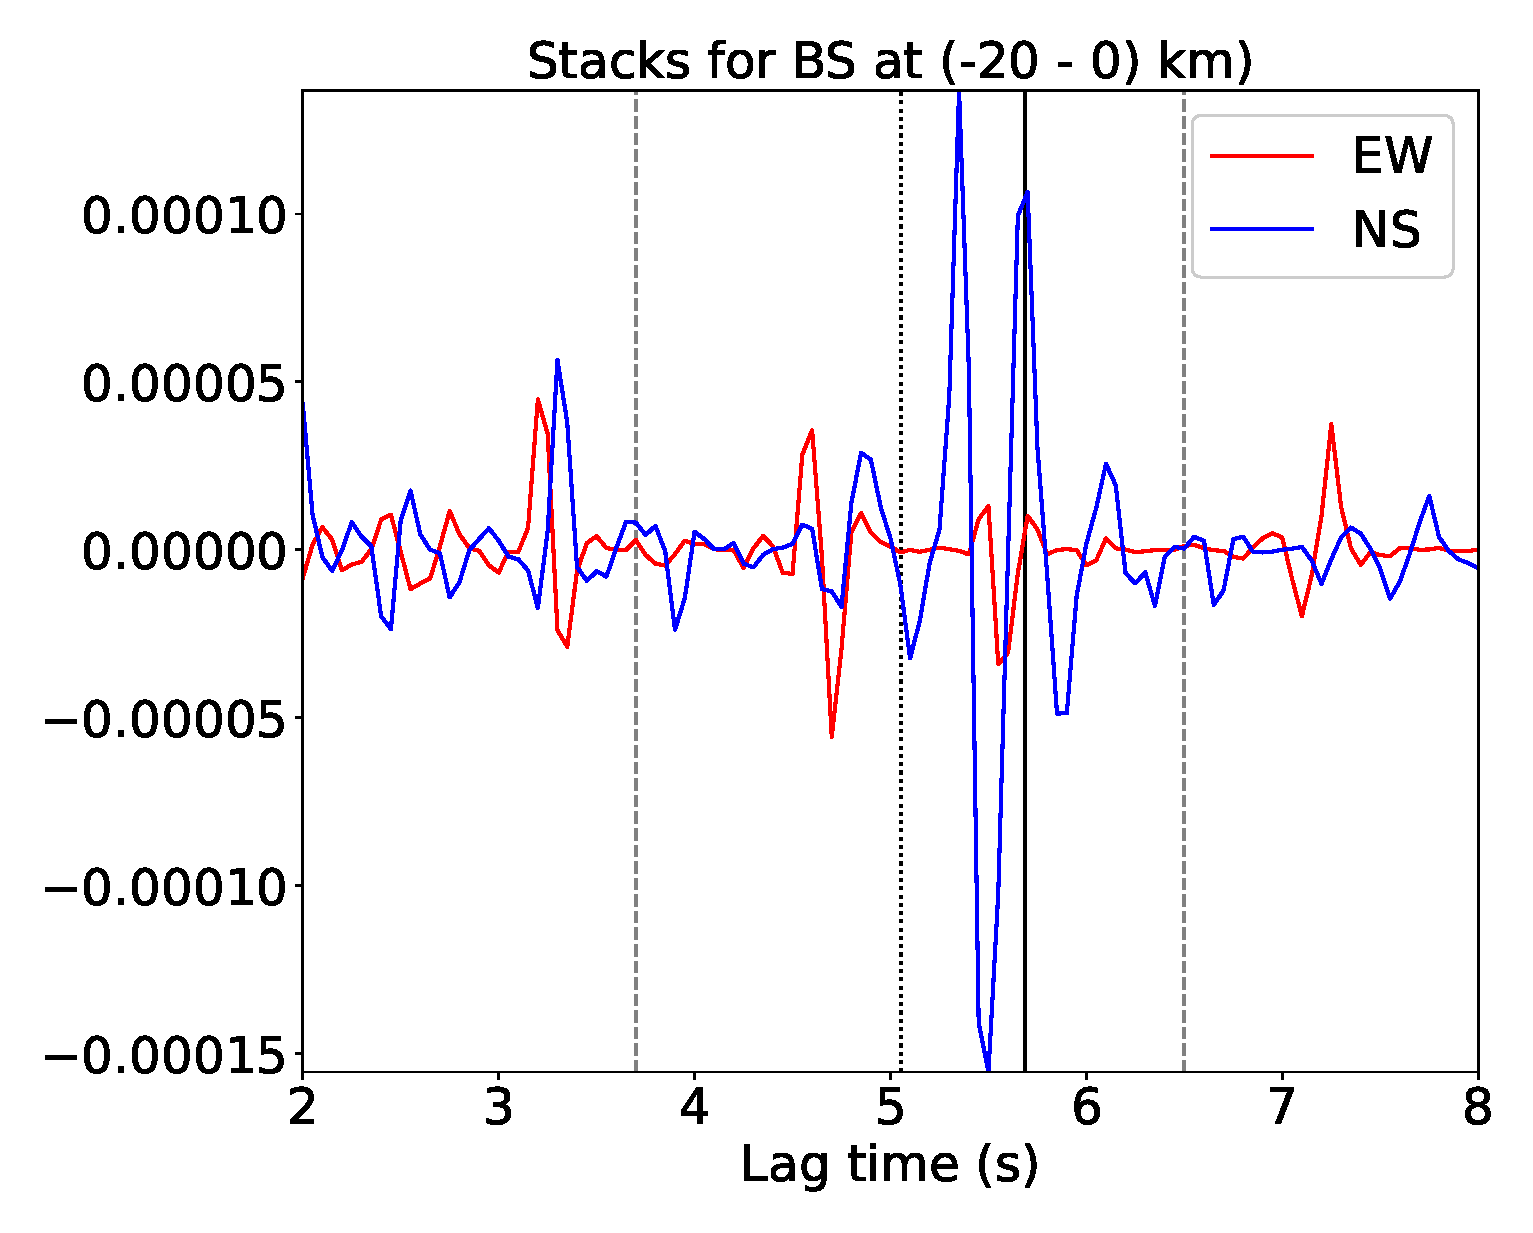
\includegraphics[width=\linewidth]{figures/intervals/BS_-20_000_stacks.eps}
\caption{See caption of Figure 1 for an explanation of this figure.}
\end{figure}

\begin{figure}[H]
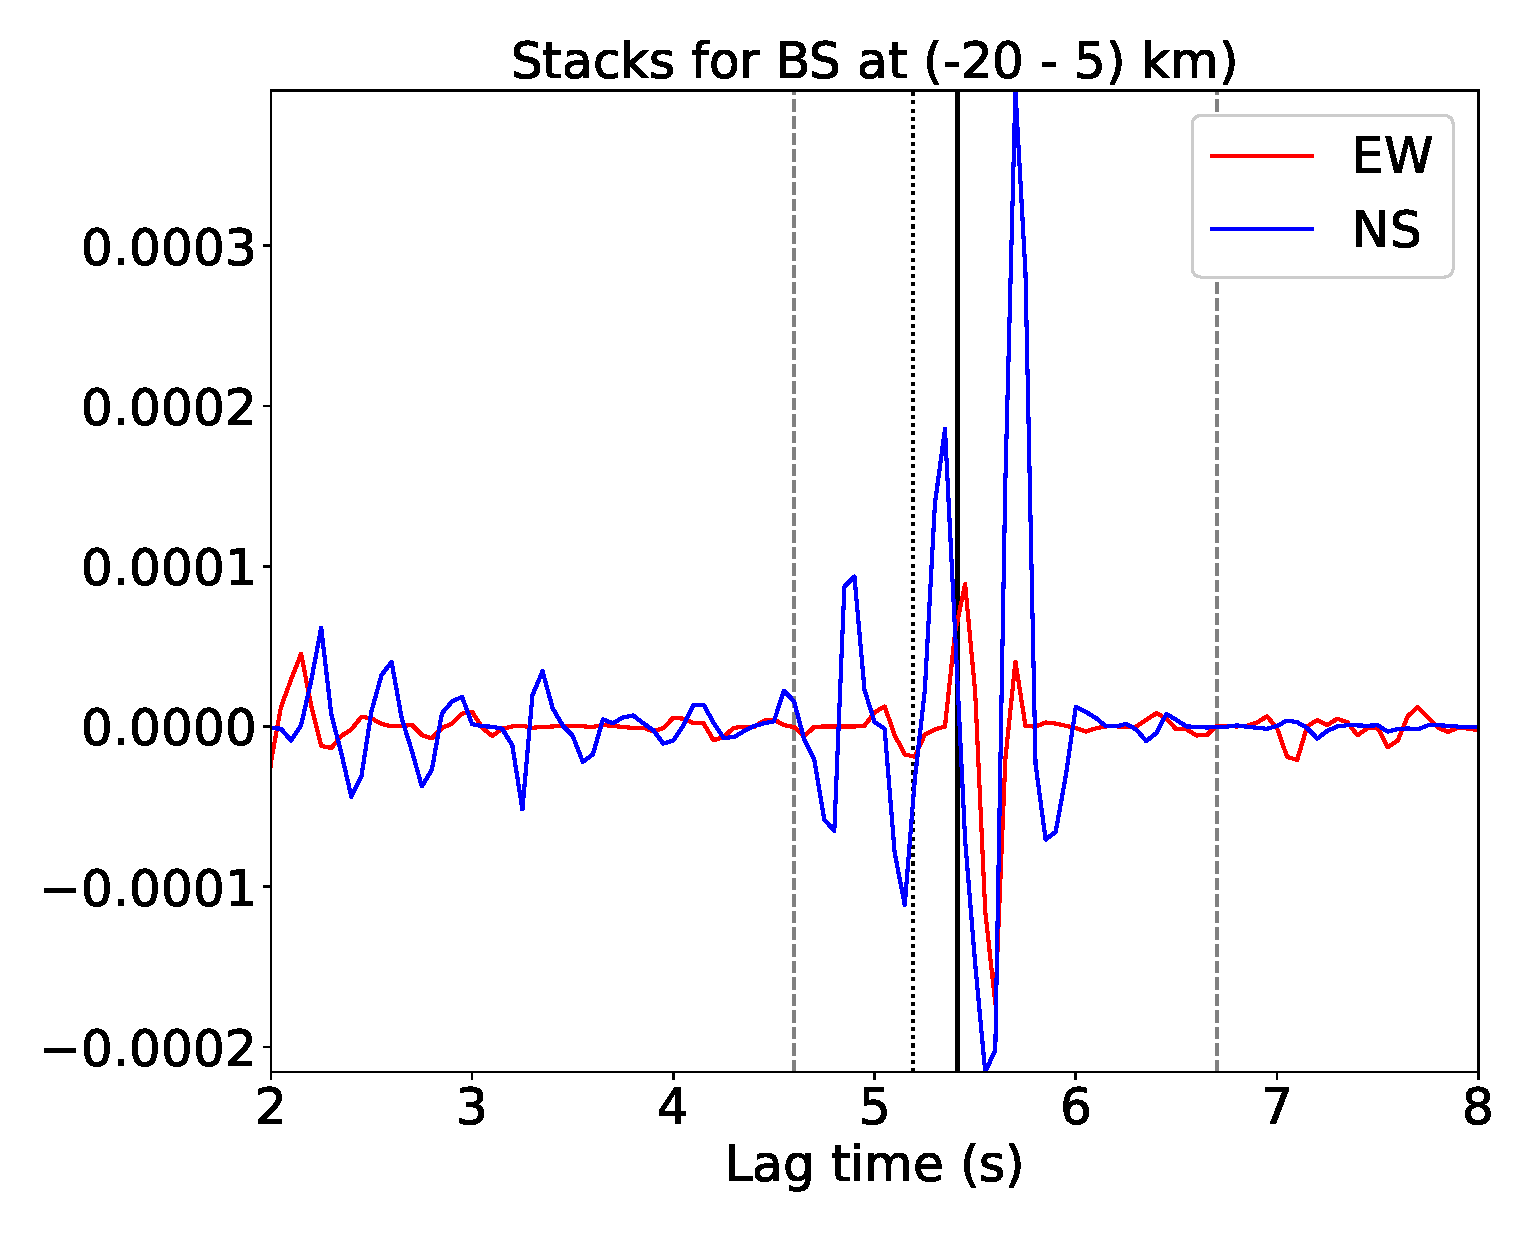
\includegraphics[width=\linewidth]{figures/intervals/BS_-20_005_stacks.eps}
\caption{See caption of Figure 1 for an explanation of this figure.}
\end{figure}

\begin{figure}[H]
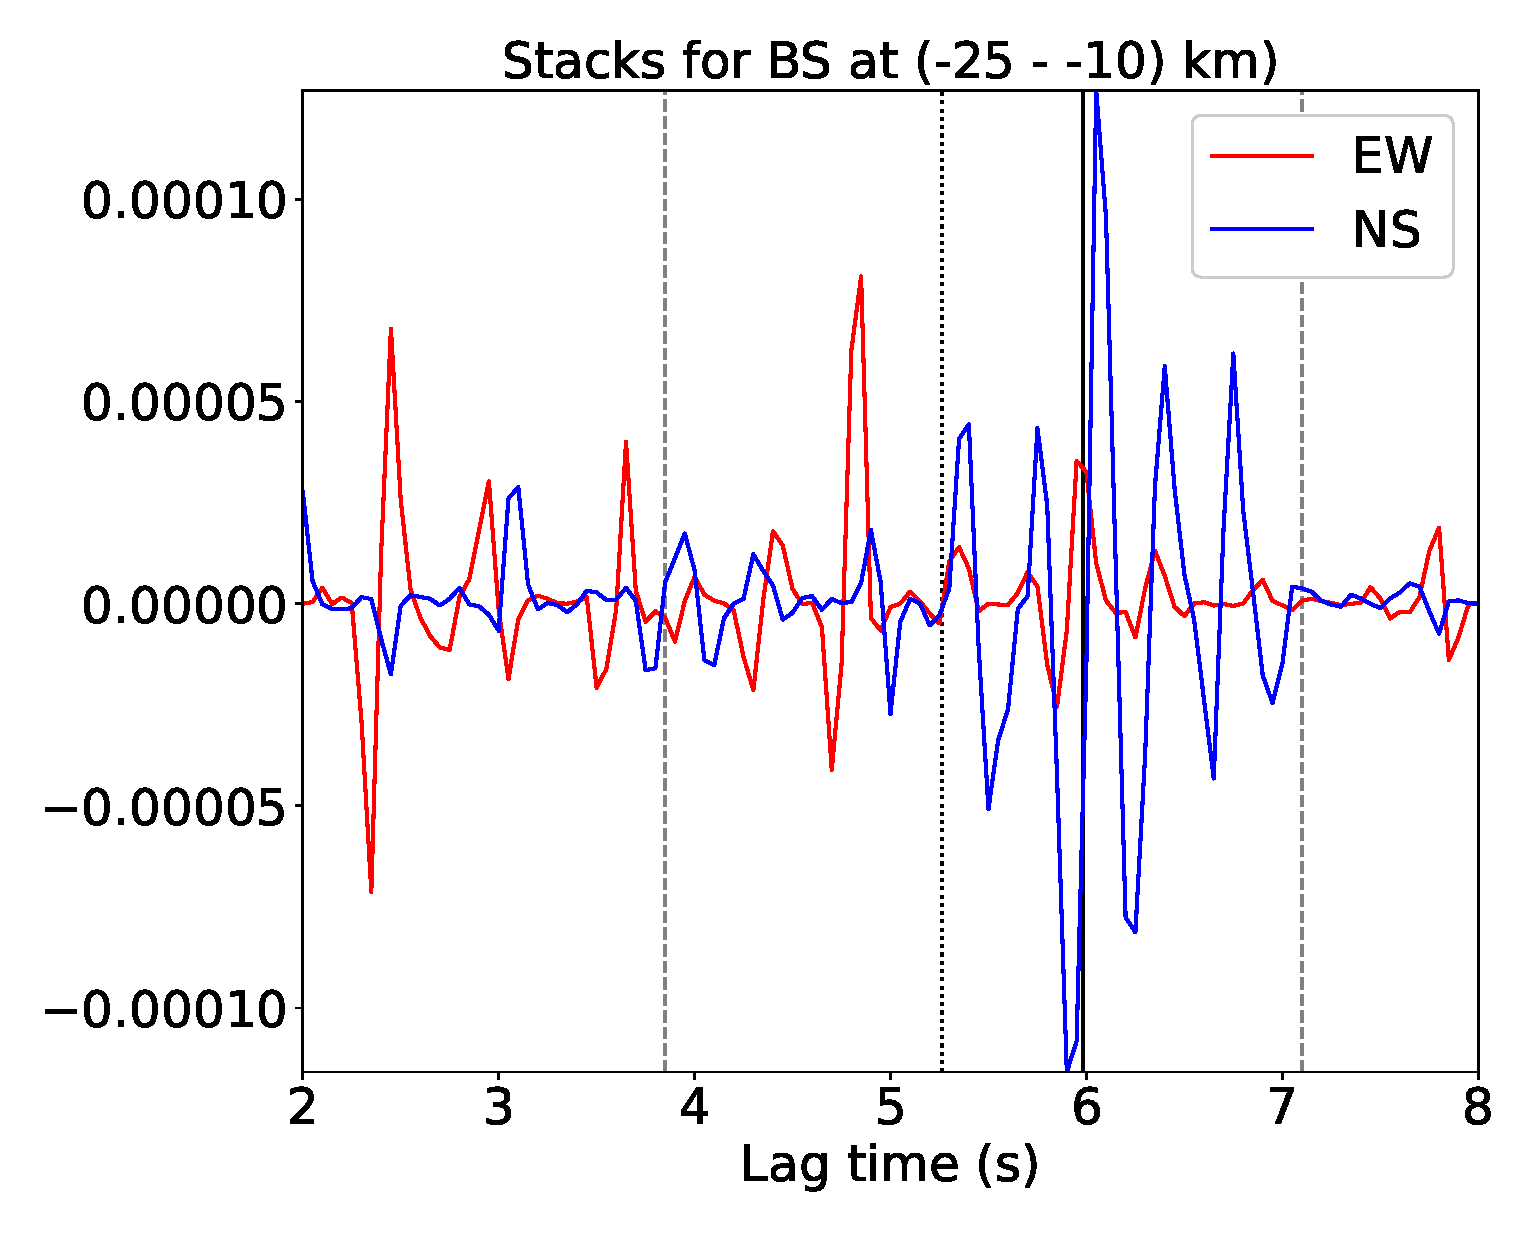
\includegraphics[width=\linewidth]{figures/intervals/BS_-25_-10_stacks.eps}
\caption{See caption of Figure 1 for an explanation of this figure.}
\end{figure}

\begin{figure}[H]
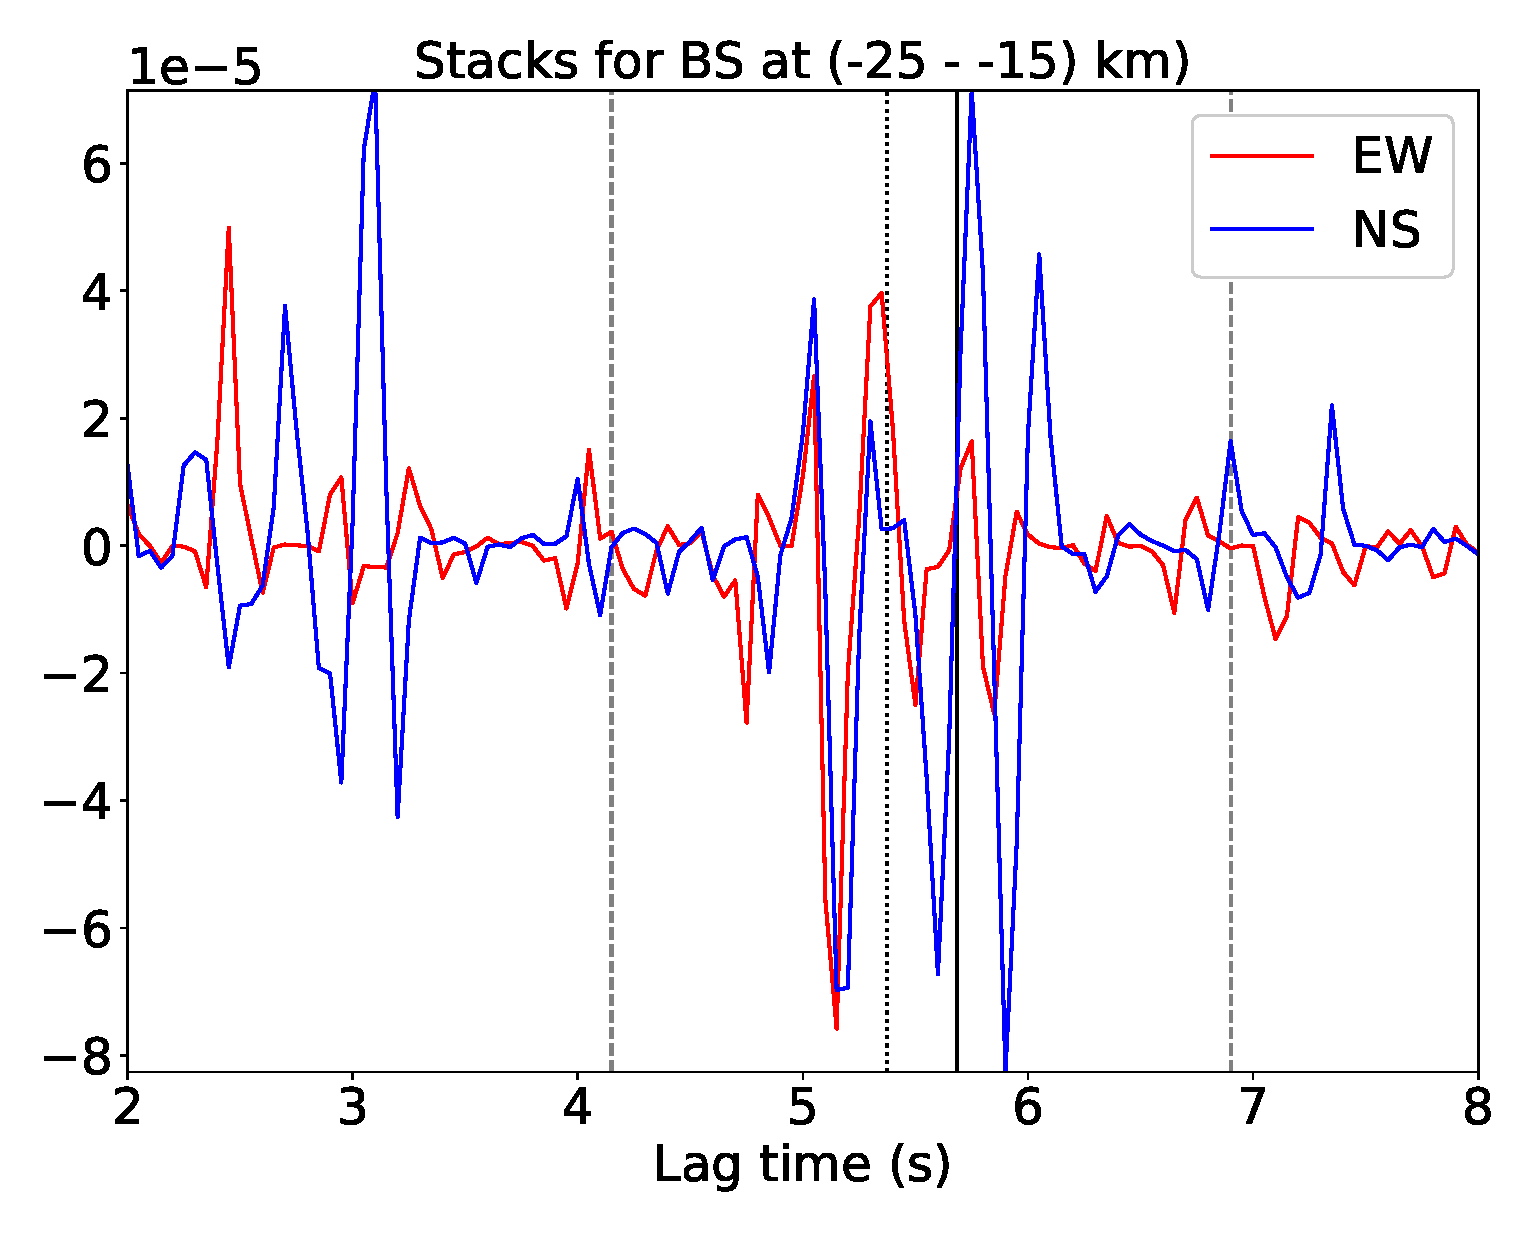
\includegraphics[width=\linewidth]{figures/intervals/BS_-25_-15_stacks.eps}
\caption{See caption of Figure 1 for an explanation of this figure.}
\end{figure}

\begin{figure}[H]
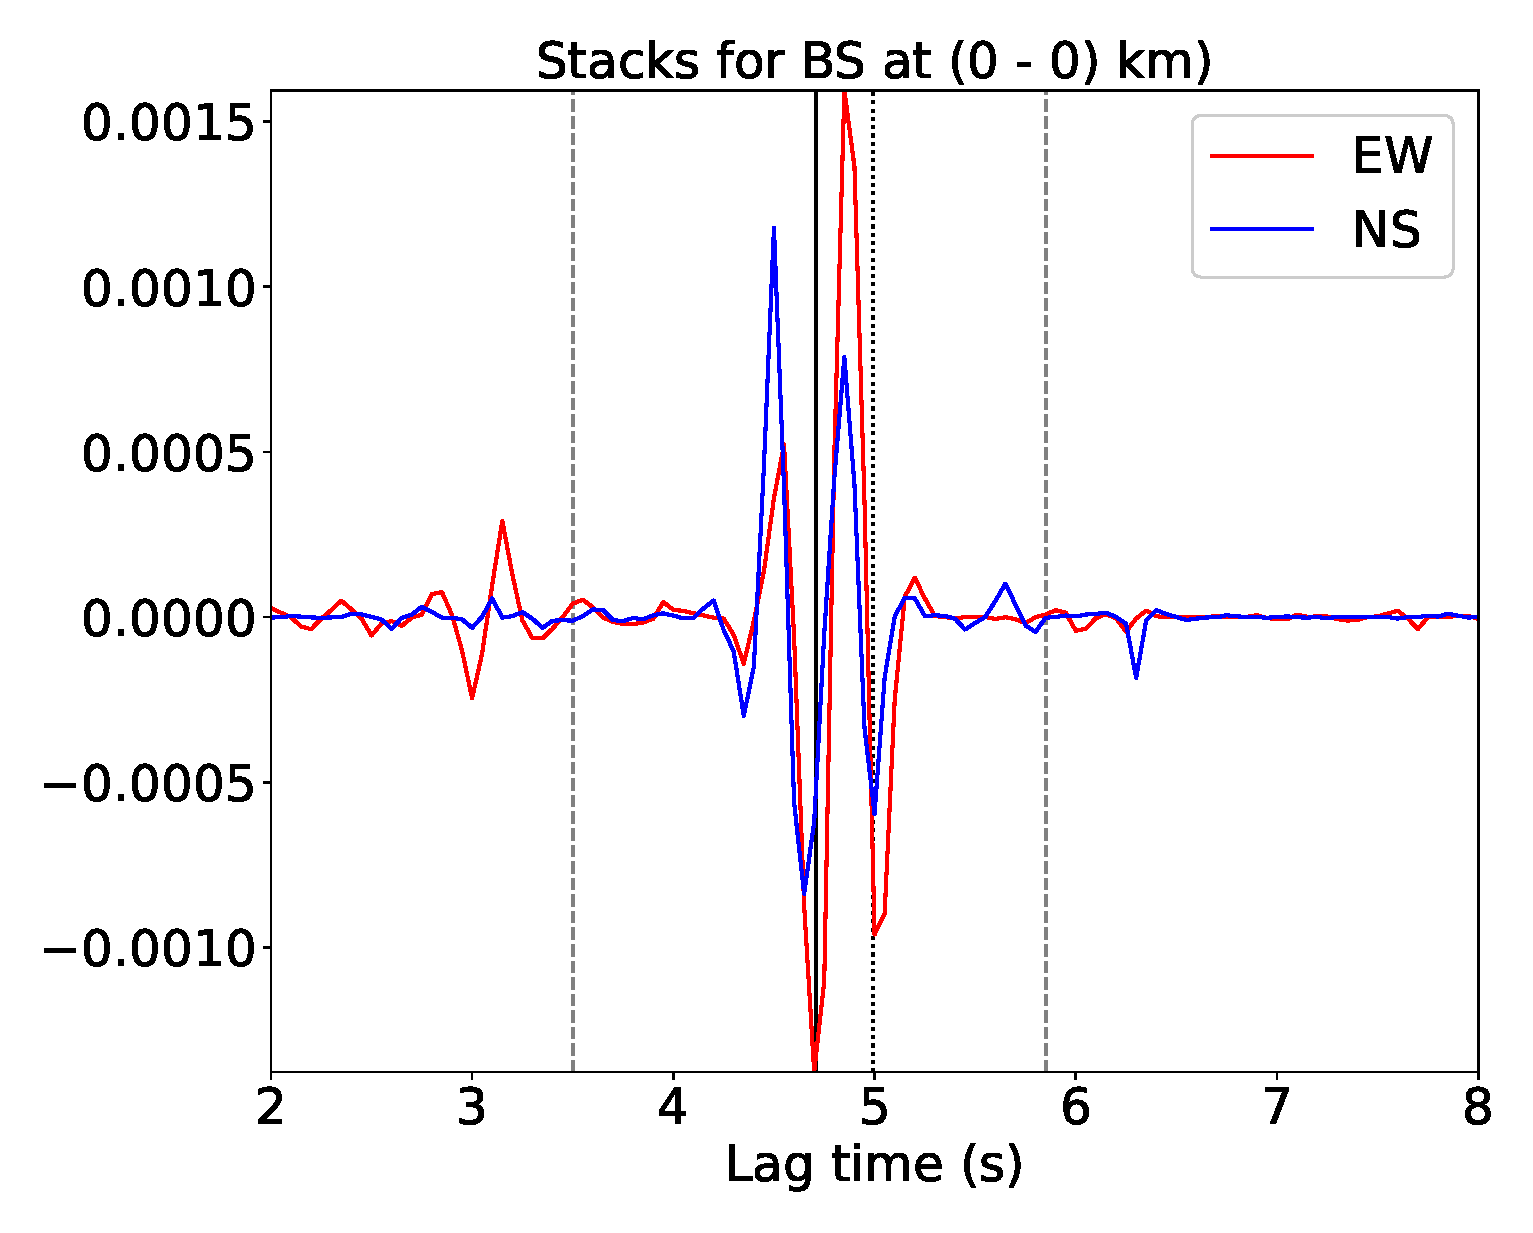
\includegraphics[width=\linewidth]{figures/intervals/BS_000_000_stacks.eps}
\caption{See caption of Figure 1 for an explanation of this figure.}
\end{figure}

\begin{figure}[H]
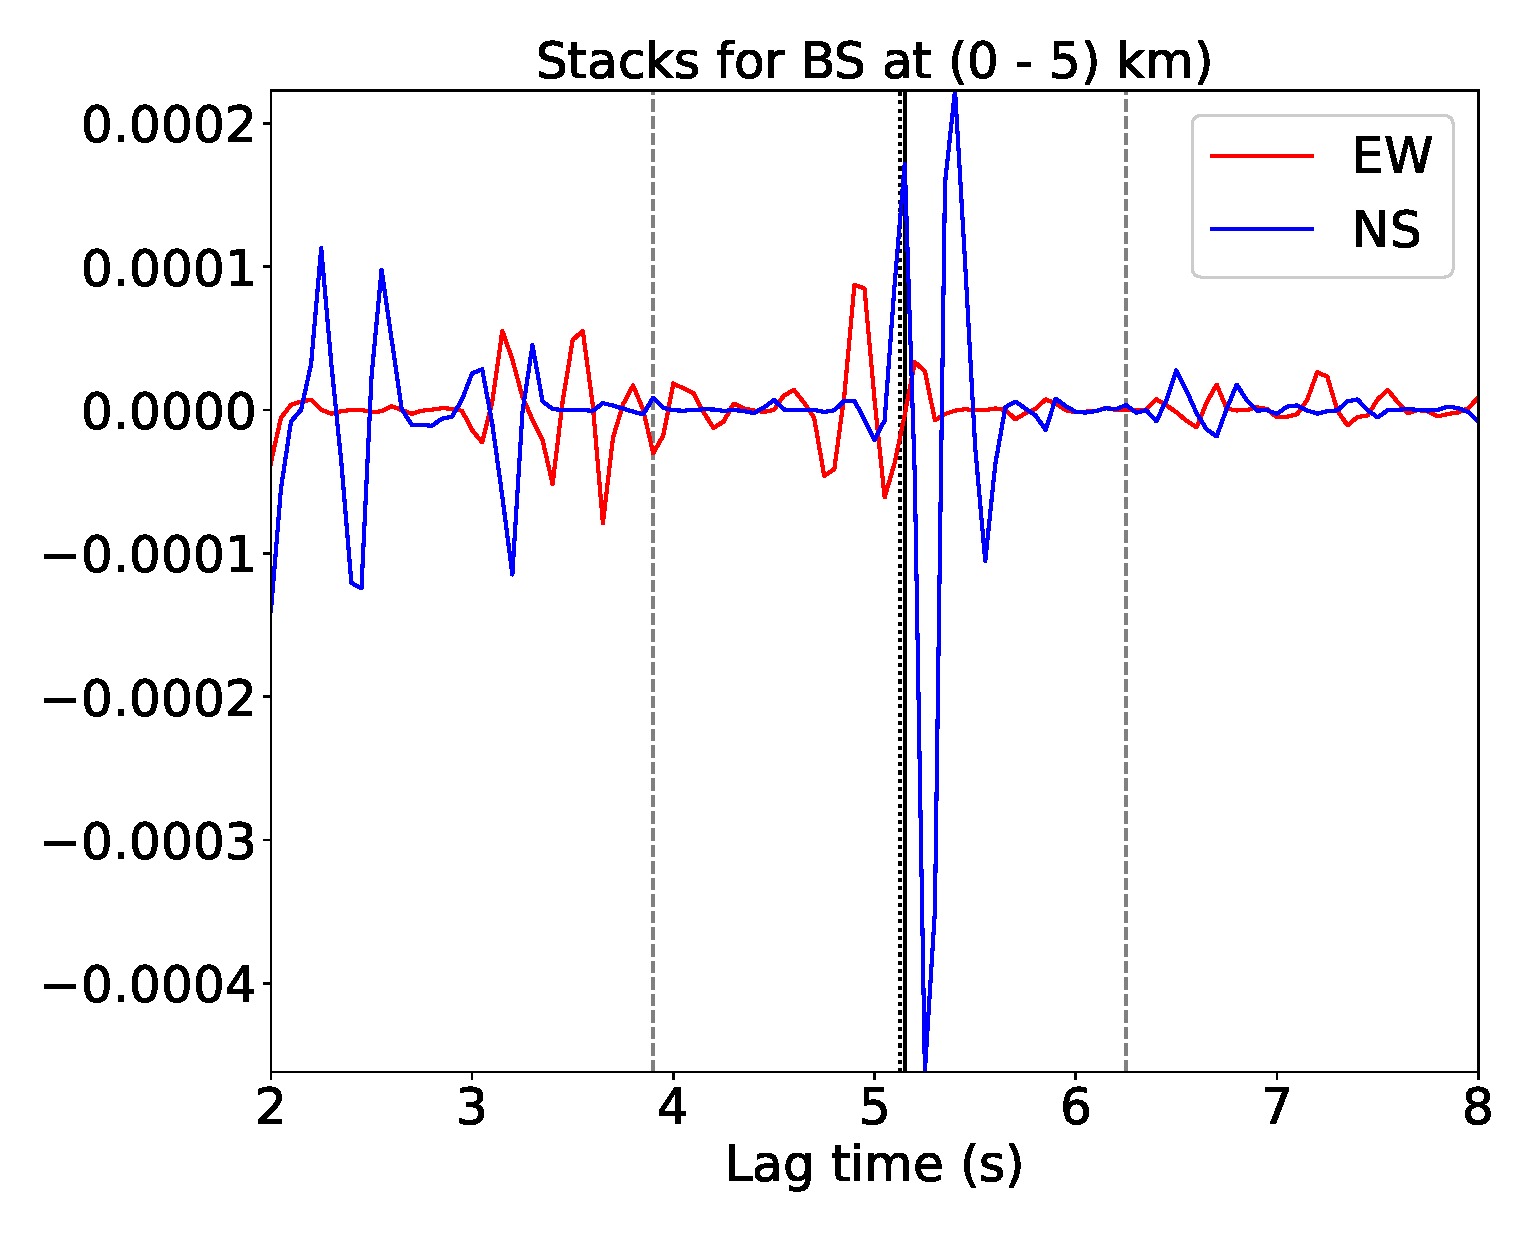
\includegraphics[width=\linewidth]{figures/intervals/BS_000_005_stacks.eps}
\caption{See caption of Figure 1 for an explanation of this figure.}
\end{figure}

\begin{figure}[H]
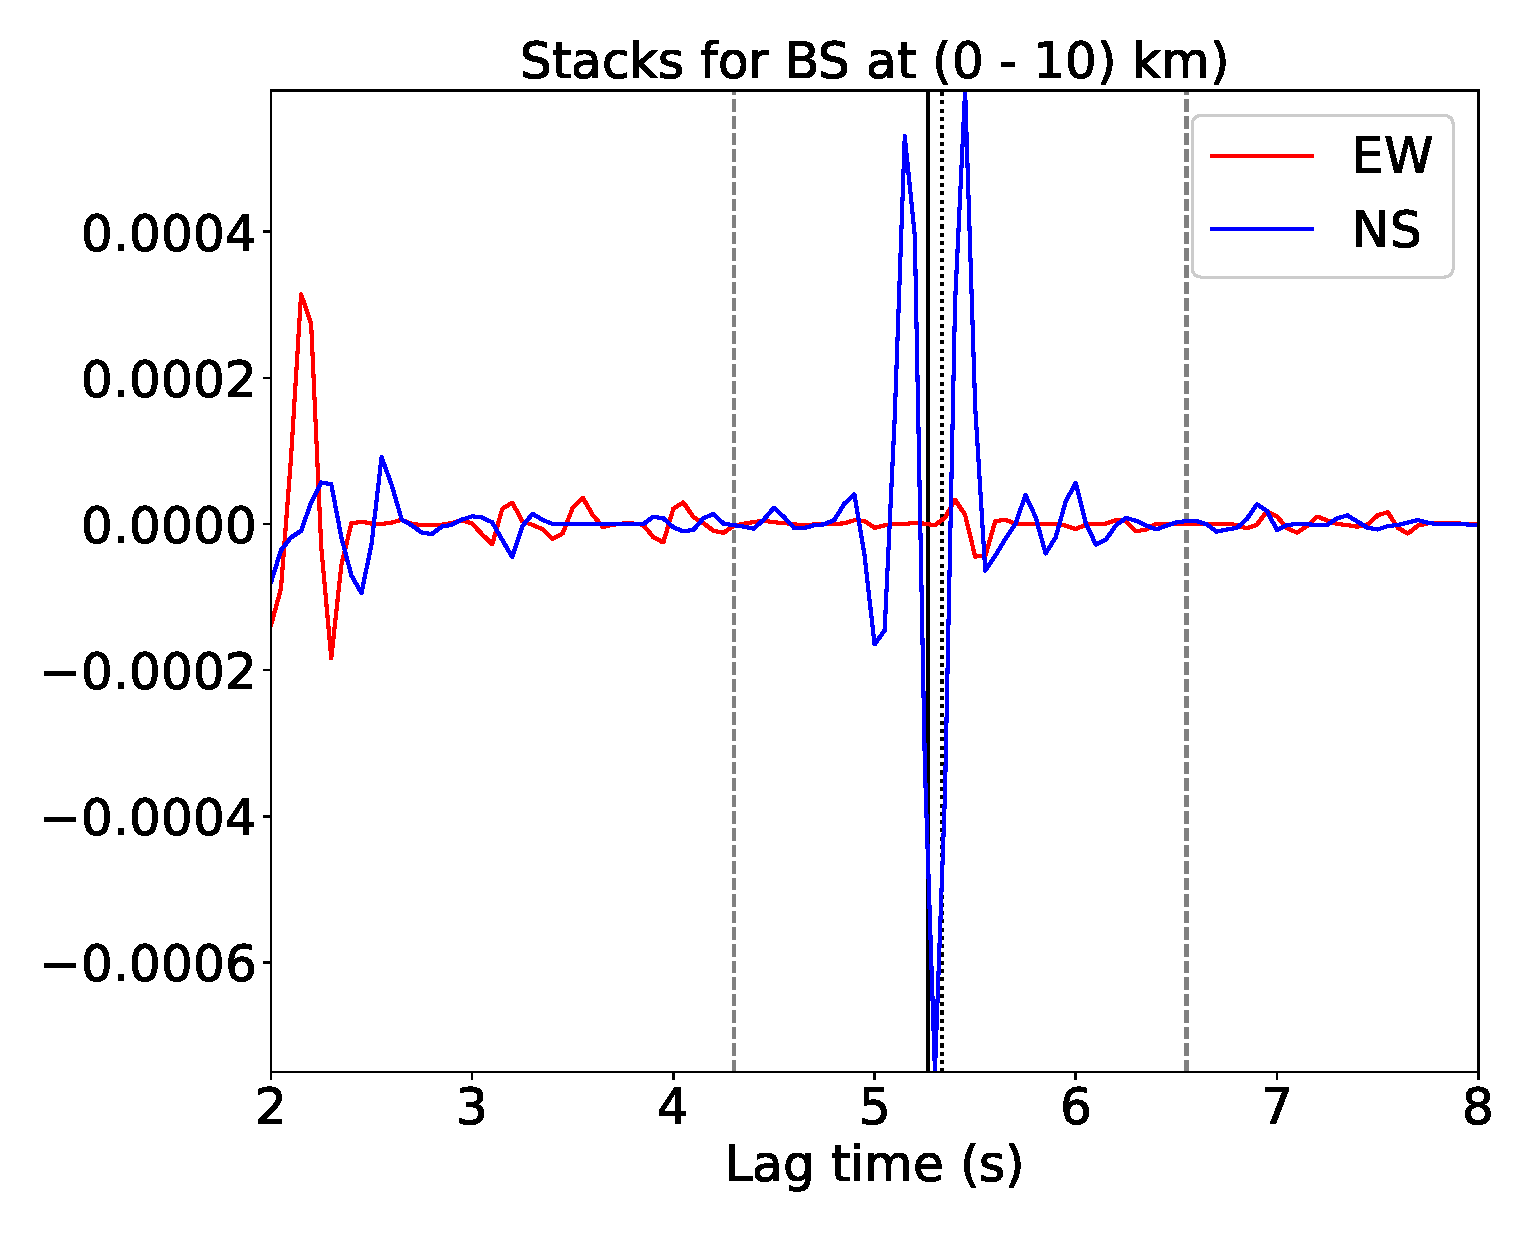
\includegraphics[width=\linewidth]{figures/intervals/BS_000_010_stacks.eps}
\caption{See caption of Figure 1 for an explanation of this figure.}
\end{figure}

\begin{figure}[H]
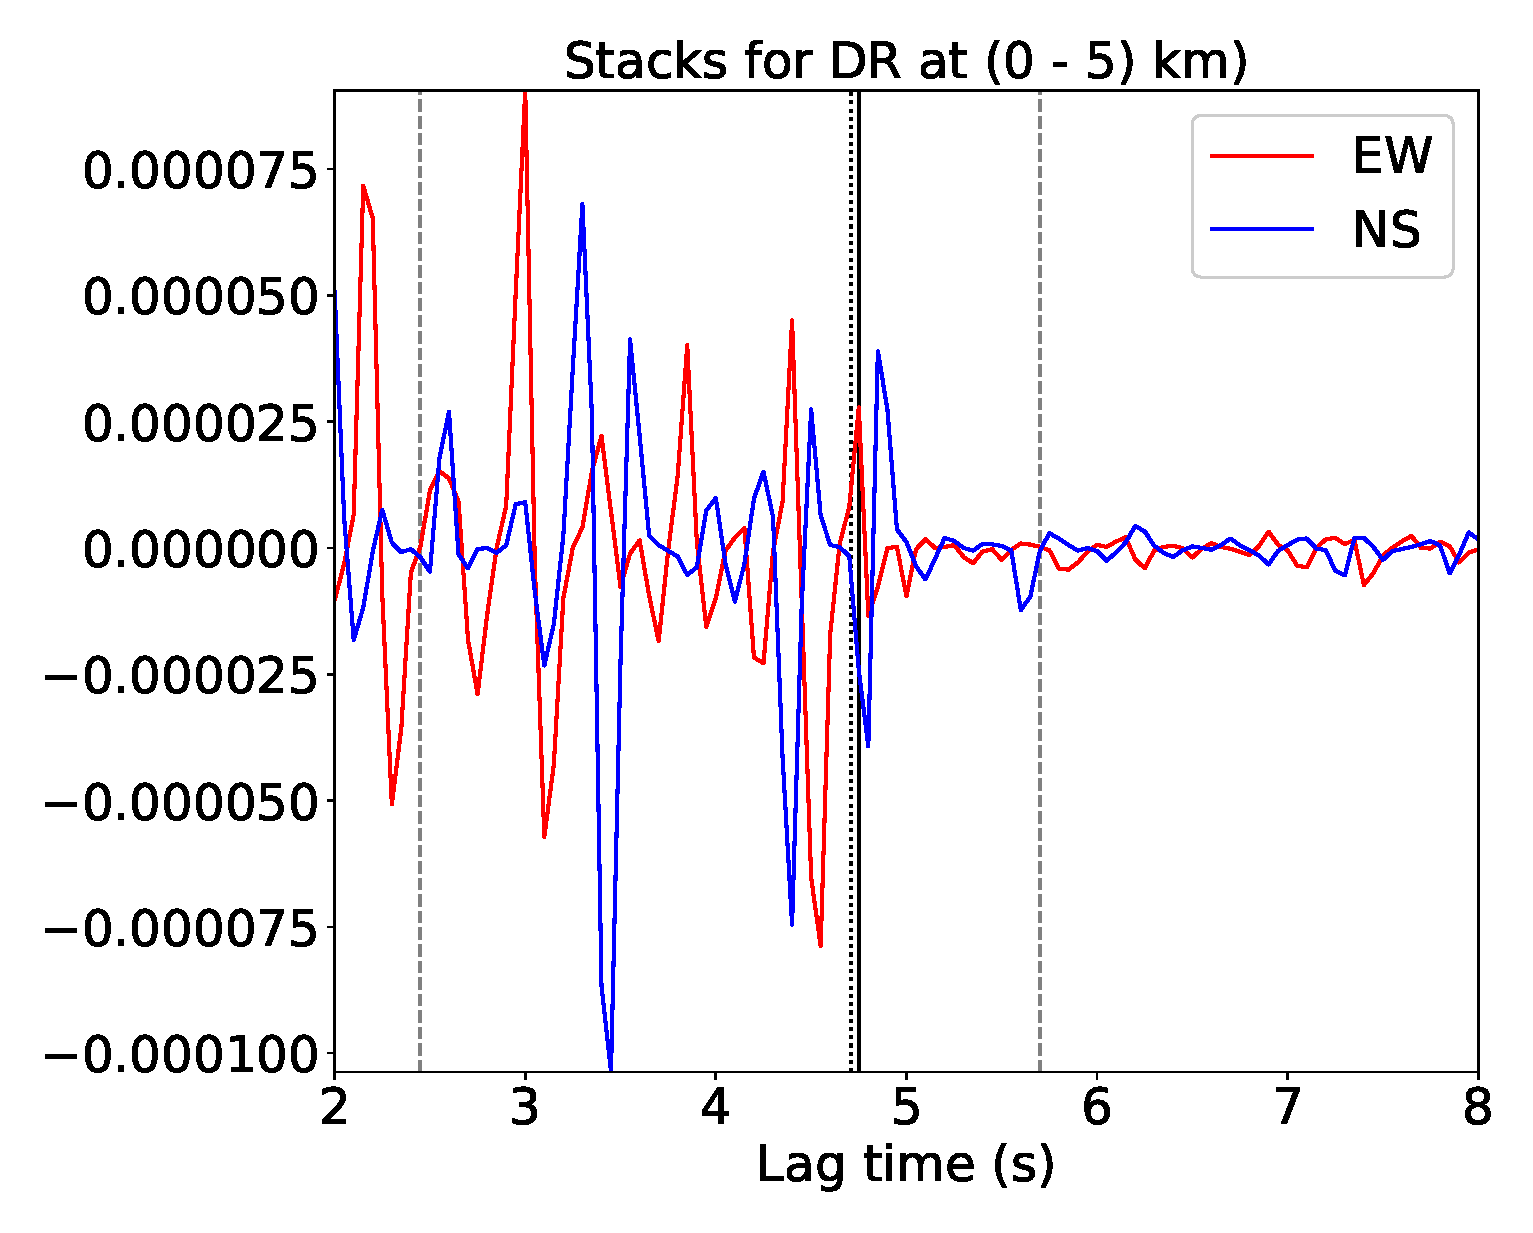
\includegraphics[width=\linewidth]{figures/intervals/DR_000_005_stacks.eps}
\caption{See caption of Figure 1 for an explanation of this figure.}
\end{figure}

\begin{figure}[H]
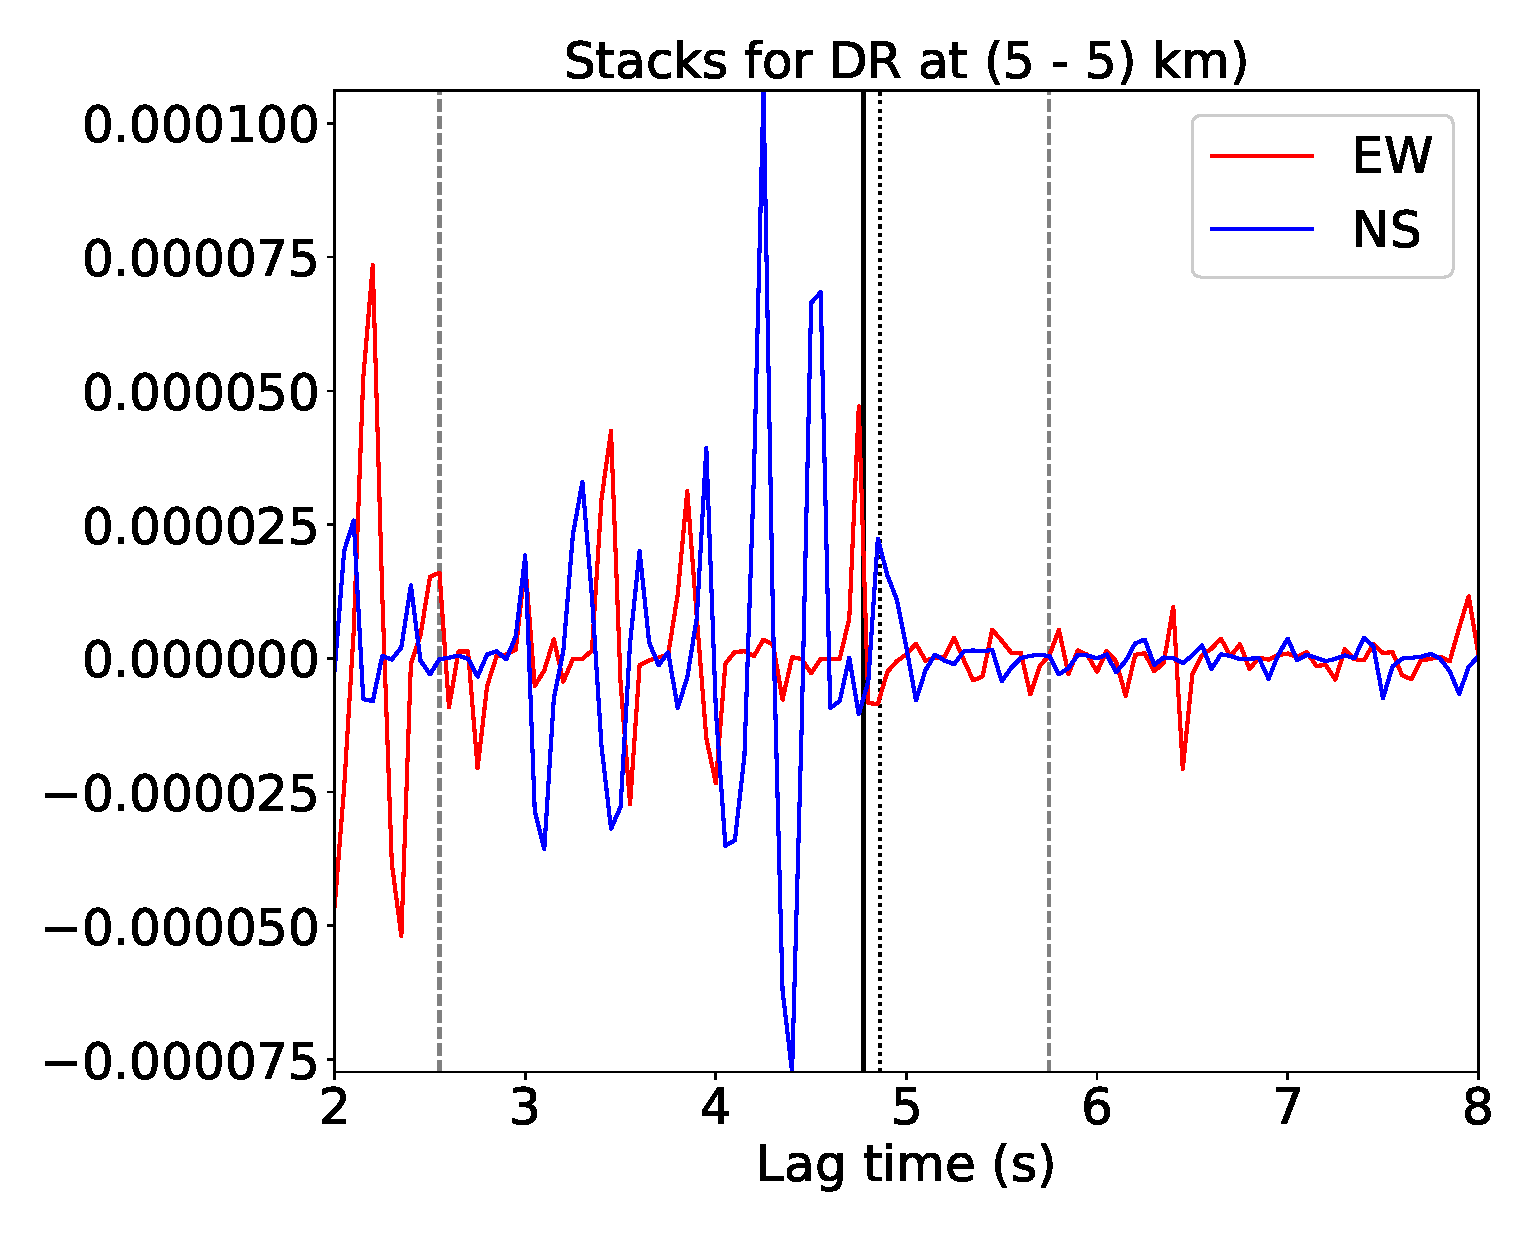
\includegraphics[width=\linewidth]{figures/intervals/DR_005_005_stacks.eps}
\caption{See caption of Figure 1 for an explanation of this figure.}
\end{figure}

\begin{figure}[H]
\includegraphics[width=\linewidth]{figures/intervals/DR_005_010_stacks.eps}
\caption{See caption of Figure 1 for an explanation of this figure.}
\end{figure}

\begin{figure}[H]
\includegraphics[width=\linewidth]{figures/intervals/DR_005_020_stacks.eps}
\caption{See caption of Figure 1 for an explanation of this figure.}
\end{figure}

\begin{figure}[H]
\includegraphics[width=\linewidth]{figures/intervals/DR_005_025_stacks.eps}
\caption{See caption of Figure 1 for an explanation of this figure.}
\end{figure}

\begin{figure}[H]
\includegraphics[width=\linewidth]{figures/intervals/DR_010_010_stacks.eps}
\caption{See caption of Figure 1 for an explanation of this figure.}
\end{figure}

\begin{figure}[H]
\includegraphics[width=\linewidth]{figures/intervals/DR_010_015_stacks.eps}
\caption{See caption of Figure 1 for an explanation of this figure.}
\end{figure}

\begin{figure}[H]
\includegraphics[width=\linewidth]{figures/intervals/DR_010_020_stacks.eps}
\caption{See caption of Figure 1 for an explanation of this figure.}
\end{figure}

\begin{figure}[H]
\includegraphics[width=\linewidth]{figures/intervals/GC_010_010_stacks.eps}
\caption{See caption of Figure 1 for an explanation of this figure.}
\end{figure}

\begin{figure}[H]
\includegraphics[width=\linewidth]{figures/intervals/GC_010_015_stacks.eps}
\caption{See caption of Figure 1 for an explanation of this figure.}
\end{figure}

\begin{figure}[H]
\includegraphics[width=\linewidth]{figures/intervals/PA_-05_000_stacks.eps}
\caption{See caption of Figure 1 for an explanation of this figure.}
\end{figure}

\begin{figure}[H]
\includegraphics[width=\linewidth]{figures/intervals/PA_000_000_stacks.eps}
\caption{See caption of Figure 1 for an explanation of this figure.}
\end{figure}

\begin{figure}[H]
\includegraphics[width=\linewidth]{figures/intervals/TB_-05_-05_stacks.eps}
\caption{See caption of Figure 1 for an explanation of this figure.}
\end{figure}

\begin{figure}[H]
\includegraphics[width=\linewidth]{figures/intervals/TB_-05_-10_stacks.eps}
\caption{See caption of Figure 1 for an explanation of this figure.}
\end{figure}

\begin{figure}[H]
\includegraphics[width=\linewidth]{figures/intervals/TB_-05_-15_stacks.eps}
\caption{See caption of Figure 1 for an explanation of this figure.}
\end{figure}

\begin{figure}[H]
\includegraphics[width=\linewidth]{figures/intervals/TB_-05_-20_stacks.eps}
\caption{See caption of Figure 1 for an explanation of this figure.}
\end{figure}

\begin{figure}[H]
\includegraphics[width=\linewidth]{figures/intervals/TB_-05_-25_stacks.eps}
\caption{See caption of Figure 1 for an explanation of this figure.}
\end{figure}

\begin{figure}[H]
\includegraphics[width=\linewidth]{figures/intervals/TB_-10_-05_stacks.eps}
\caption{See caption of Figure 1 for an explanation of this figure.}
\end{figure}

\begin{figure}[H]
\includegraphics[width=\linewidth]{figures/intervals/TB_-10_-10_stacks.eps}
\caption{See caption of Figure 1 for an explanation of this figure.}
\end{figure}

\begin{figure}[H]
\includegraphics[width=\linewidth]{figures/intervals/TB_-10_-15_stacks.eps}
\caption{See caption of Figure 1 for an explanation of this figure.}
\end{figure}

\begin{figure}[H]
\includegraphics[width=\linewidth]{figures/intervals/TB_-10_-20_stacks.eps}
\caption{See caption of Figure 1 for an explanation of this figure.}
\end{figure}

\begin{figure}[H]
\includegraphics[width=\linewidth]{figures/intervals/TB_-15_000_stacks.eps}
\caption{See caption of Figure 1 for an explanation of this figure.}
\end{figure}

\begin{figure}[H]
\includegraphics[width=\linewidth]{figures/intervals/TB_000_-05_stacks.eps}
\caption{See caption of Figure 1 for an explanation of this figure.}
\end{figure}

\begin{figure}[H]
\includegraphics[width=\linewidth]{figures/intervals/TB_000_-10_stacks.eps}
\caption{See caption of Figure 1 for an explanation of this figure.}
\end{figure}

\begin{figure}[H]
\includegraphics[width=\linewidth]{figures/intervals/TB_005_-05_stacks.eps}
\caption{See caption of Figure 1 for an explanation of this figure.}
\end{figure}

\begin{figure}[H]
\includegraphics[width=\linewidth]{figures/intervals/TB_005_000_stacks.eps}
\caption{See caption of Figure 1 for an explanation of this figure.}
\end{figure}

\begin{figure}[H]
\includegraphics[width=\linewidth]{figures/intervals/TB_010_-05_stacks.eps}
\caption{See caption of Figure 1 for an explanation of this figure.}
\end{figure}

\begin{figure}[H]
\includegraphics[width=\linewidth]{figures/intervals/TB_010_-10_stacks.eps}
\caption{See caption of Figure 1 for an explanation of this figure.}
\end{figure}

\begin{figure}[H]
\includegraphics[width=\linewidth]{figures/intervals/TB_015_-05_stacks.eps}
\caption{See caption of Figure 1 for an explanation of this figure.}
\end{figure}

\end{document}